
\documentclass[12pt,a4paper]{ctexrep}
\usepackage{amsmath,amssymb}
\usepackage{fontspec}
\xeCJKsetup{AutoFallBack = true}
\setCJKfallbackfamilyfont\CJKrmdefault{Malgun Gothic}[Scale=MatchLowercase]
\setCJKfallbackfamilyfont\CJKsfdefault{Malgun Gothic}[Scale=MatchLowercase]
\setCJKfallbackfamilyfont\CJKttdefault{Malgun Gothic}[Scale=MatchLowercase]
\usepackage[top=1.5cm,bottom=1.5cm,left=1cm,right=1cm,headheight=15pt]{geometry}
\usepackage{pdflscape}

\usepackage{hyperref}
\usepackage{graphicx}
\usepackage{tikz}
\usetikzlibrary{shapes.multipart, shapes.geometric, shapes.arrows, decorations.pathreplacing, arrows.meta, positioning, matrix, calc}
\usepackage{float}
\usepackage{booktabs}
\usepackage{tabularx}
\usepackage{tabulary}
\usepackage{pgfplots}
\pgfplotsset{compat=1.18}
\usepackage{setspace}
\usepackage{fancyhdr}
\usepackage{algorithm}
\usepackage{algpseudocode}
\usepackage{needspace}
\usepackage{etoolbox}
\usepackage{listings}
\widowpenalty=10000
\clubpenalty=10000
\raggedbottom
\emergencystretch=3em
\tolerance=2000
\setlength{\intextsep}{8pt}
\setlength{\textfloatsep}{10pt}
\pretocmd{\section}{\needspace{13\baselineskip}}{}{}
\pretocmd{\subsection}{\needspace{8\baselineskip}}{}{}
\pretocmd{\subsubsection}{\needspace{5\baselineskip}}{}{}

\lstset{
    basicstyle=\ttfamily\small,
    numbers=left,
    numberstyle=\tiny,
    frame=single,
    breaklines=true,
    showstringspaces=false,
    tabsize=4
}

\onehalfspacing
\pagestyle{fancy}
\fancyhf{}

\hypersetup{
    colorlinks=true,
    linkcolor=black,
    citecolor=black,
    urlcolor=blue
}

\title{\textbf{\huge 计算机网络}}
\author{}
\date{}

\begin{document}

\clearpage
\thispagestyle{empty}
\vspace*{\fill}

\begin{center}
{\huge 计算机网络}\\[0.8em]
{\large Computer Networking}\\[2.5em]
{\large MS Roslyn}\\[0.6em]
{\large \today}
\end{center}

\vspace{2.5em}

\begin{center}
{\bfseries 摘要}
\end{center}

\vspace{1em}

\begin{center}
本教程采用自顶向下的视角系统讲解计算机网络：从应用层协议出发，逐层深入到运输层、网络层（数据平面与控制平面）、链路层，并覆盖无线与移动网络以及网络安全。教程强调「分层 + 协议 + 性能」三条主线，用可计算的公式与可交互的例子说明时延、吞吐、可靠传输、拥塞控制、路由与转发、差错检测、密钥交换等核心机制，帮助读者建立贯穿五层模型的完整心智模型。
\end{center}

\vspace*{\fill}
\clearpage

\tableofcontents
\newpage

\clearpage
\clearpage
\begingroup
\let\clearpage\relax
\let\cleardoublepage\relax
\vspace*{\fill}
\chapter{计算机网络概述与体系结构}
\begin{center}
网络是一张把「主机」用「链路」与「交换设备」连起来的图；协议是通信双方对「时序 + 格式 + 语义」的约定。本章先建立「边缘--核心--性能--分层」四块基石。
\end{center}
\vspace*{\fill}
\endgroup
\clearpage

\section{网络的组成：边缘、接入与核心}

\subsection{动机}
为什么要先谈「组成」？因为一个网络系统的所有问题——带宽够不够、时延大不大、故障如何隔离、安全边界在哪里——都可以归结为「谁处在网络的哪个位置」。只有先把庞杂的互联网抽象成\textbf{端系统}、\textbf{接入网}与\textbf{网络核心}三块，后续的协议设计才有讨论的坐标系。

\subsection{形式化定义}
把网络建模为一个图 $G=(V,E)$：顶点集合 $V$ 包含\textbf{端系统 (end system / host)}与\textbf{分组交换机 (packet switch)}，边集合 $E$ 为通信\textbf{链路 (link)}。每条链路带有两个属性：速率 $R$（bit/s）与传播时延 $d_{\text{prop}}$。端系统之间的一条「路径」就是图中的一条路 (path)：

\begin{equation}
    \text{path} = \langle v_0, e_1, v_1, e_2, \dots, e_k, v_k \rangle, \qquad v_0, v_k \in \text{Hosts}.
\end{equation}

据此，网络可划分为三个逻辑区域：

\begin{itemize}
    \item \textbf{网络边缘 (Network Edge)}：端系统 (host)，包括主机、服务器、手机、传感器、物联网设备。它们运行应用程序，是「产生与消费」数据的地方，一般不参与转发。
    \item \textbf{接入网 (Access Network)}：把边缘连接到核心的\textbf{第一跳}，如 DSL、HFC、FTTH、以太网、Wi-Fi、蜂窝 (4G/5G)。它决定用户「入口速率」。
    \item \textbf{网络核心 (Network Core)}：由分组交换机、路由器及高速链路组成的网状骨干，负责把分组从一条链路转发到另一条链路。
\end{itemize}

\begin{figure}[H]
\centering
\begin{tikzpicture}[
    host/.style={draw, rounded corners, minimum width=1.5cm, minimum height=0.7cm, font=\small, align=center},
    cloud/.style={draw, ellipse, minimum width=2.4cm, minimum height=1.3cm, font=\small, align=center},
    link/.style={draw, thick, -{Latex[length=2mm]}}
]
    \node[host] (h1) at (0,1.2) {主机};
    \node[host] (h2) at (0,-1.2) {手机};
    \node[cloud] (acc) at (3,0) {接入网};
    \node[cloud] (core) at (6.8,0) {网络核心};
    \node[host] (srv) at (10,0) {服务器};

    \draw[link] (h1) -- (acc);
    \draw[link] (h2) -- (acc);
    \draw[link] (acc) -- (core);
    \draw[link] (core) -- (srv);

    \node[font=\scriptsize, below] at (0,-1.9) {边缘};
    \node[font=\scriptsize, below] at (3,-1.1) {接入};
    \node[font=\scriptsize, below] at (6.8,-1.1) {核心};
\end{tikzpicture}
\caption{边缘--接入--核心的三段式结构}
\label{fig:edge_access_core}
\end{figure}

\subsection{接入技术详细对比}
接入技术可沿四个维度区分：\textbf{介质}、\textbf{标称速率}、\textbf{共享方式}（独享还是争用）、\textbf{双工方式}（全双工/半双工）。

\begin{table}[H]
\centering
\caption{常见接入技术对比（速率、介质、共享方式、双工）}
\begin{tabulary}{\textwidth}{CCCCC}
\toprule
技术 & 介质 & 典型速率 & 共享方式 & 双工 \\
\midrule
DSL & 电话双绞线 & 24--52 Mbps 下行 & 用户独享（局端汇聚共享） & 全双工（FDD） \\
HFC & 同轴电缆 + 光纤 & 数十--数百 Mbps & 上行为用户争用 & 频分上下行 \\
FTTH & 光纤 & 1 Gbps 以上 & PON 上行为共享/时分 & 全双工 \\
Wi-Fi & 2.4/5/6 GHz 无线 & 数百 Mbps--Gbps & 共享介质、CSMA/CA & 半双工 \\
蜂窝 4G/5G & 授权频段无线 & 数十 Mbps--Gbps & 小区内共享调度 & 全双工（FDD/TDD） \\
\bottomrule
\end{tabulary}
\end{table}

\textbf{要点解读：}「共享方式」直接决定\textbf{有效速率随用户数下降}的方式。HFC 上行与 Wi-Fi 属于\textbf{争用型}，用户越多碰撞与排队越严重；FTTH 在无源分光器后下行是广播、上行按时分复用 (TDMA) 共享。蜂窝则在基站内\textbf{集中调度}，按信道质量动态分配。

\subsection{ISP 层次结构与拓扑}

\textbf{动机：}互联网不是一张对等的图，而是由商业关系与流量交换点组织成的\textbf{层次化结构}。理解它才能理解路由为何「向上汇聚、向下分发」。

\textbf{层次：}
\begin{itemize}
    \item \textbf{Tier-1 ISP}：全球骨干，无需向他人付费即可到达全网（如 Level-3、NTT）。
    \item \textbf{Tier-2 ISP}：区域型，向 Tier-1 付费购得转接 (transit)，也与其他 Tier-2 对等 (peering)。
    \item \textbf{Tier-3 / 接入 ISP}：本地运营商，直接服务端系统。
    \item \textbf{IXP (Internet Exchange Point)}：多个 ISP 在此对等互联，降低转接成本。
    \item \textbf{内容提供商网络 (CDN)}：如大型视频网站自建骨干，与各级 ISP 就近互联、部署缓存。
\end{itemize}

\begin{figure}[H]
\centering
\begin{tikzpicture}[
    box/.style={draw, rounded corners, minimum width=2.0cm, minimum height=0.7cm, font=\small, align=center},
    ix/.style={draw, circle, minimum size=0.7cm, font=\scriptsize},
    conn/.style={draw, thick}
]
    \node[box] (t1a) at (0,3) {Tier-1 A};
    \node[box] (t1b) at (5,3) {Tier-1 B};
    \node[ix]  (ix)  at (2.5,2) {IXP};
    \node[box] (t2)  at (1,1) {Tier-2};
    \node[box] (t3)  at (4,1) {接入 ISP};
    \node[box] (cdn) at (6.5,1.6) {内容网络};

    \draw[conn] (t1a) -- (t1b);
    \draw[conn] (t1a) -- (ix);
    \draw[conn] (t1b) -- (ix);
    \draw[conn] (ix) -- (t2);
    \draw[conn] (ix) -- (t3);
    \draw[conn, dashed] (t2) -- (t3);
    \draw[conn, dashed] (cdn) -- (t1b);
    \draw[conn] (cdn) -- (t3);
\end{tikzpicture}
\caption{ISP 层次与 IXP 对等互联}
\label{fig:isp_hier}
\end{figure}

\textbf{物理拓扑形态}决定链路冗余与故障域。常见拓扑如下表；现实中骨干普遍采用\textbf{部分网状 (partial mesh)}，以兼顾冗余与成本。

\begin{table}[H]
\centering
\caption{常见网络拓扑对比}
\begin{tabulary}{\textwidth}{CCCC}
\toprule
拓扑 & 结构 & 优点 & 缺点 \\
\midrule
总线 & 单一共享介质 & 布线简单 & 冲突严重、单点失效 \\
星型 & 中心节点汇聚 & 易管理、故障隔离好 & 中心成瓶颈/单点 \\
环型 & 首尾相接 & 可双向保护 & 断链影响大 \\
网状 & 多路互联 & 高冗余、高吞吐 & 成本高、路由复杂 \\
树型 & 层次汇聚 & 扩展性好 & 上层失效影响大 \\
\bottomrule
\end{tabulary}
\end{table}

\section{交换方式：电路交换 vs 分组交换}

\subsection{动机}
端系统之间的数据要跨越许多链路，核心必须决定\textbf{如何为数据分配链路资源}。两种根本不同的答案——预留资源与按需复用——构成了网络设计的第一组对立统一。

\subsection{电路交换 (Circuit Switching)}
通信前在路径上\textbf{预留一条独占电路}，分三阶段：

\begin{enumerate}
    \item \textbf{建立 (setup)}：沿路径逐跳预留链路带宽/时隙，信令往返产生建立时延。
    \item \textbf{传输 (transfer)}：数据以恒定速率连续通过，\textbf{无排队}。
    \item \textbf{拆除 (teardown)}：释放资源。
\end{enumerate}

\textbf{优点：}时延稳定、抖动小、无需首部寻址开销。\textbf{缺点：}空闲期资源浪费；突发业务利用率低。

\subsection{分组交换 (Packet Switching)}
数据被切成\textbf{分组 (packet)}，每个分组携带首部，独立经过交换机，采用\textbf{存储转发 (store-and-forward)}：交换机必须收完整个分组才转发。核心机制是\textbf{统计多路复用}——按需占用带宽，天然适配突发流量。代价是\textbf{排队时延}与\textbf{丢包}。

\begin{figure}[H]
\centering
\begin{tikzpicture}[font=\small, xscale=1.05]
    % 电路交换时间线
    \draw[->] (0,2.0) -- (11,2.0) node[right] {$t$};
    \node[anchor=east] at (-0.2,2.0) {电路};
    \draw[fill=blue!15] (0.3,1.75) rectangle (2.0,2.25);
    \node[font=\scriptsize] at (1.15,2.0) {建立};
    \draw[fill=green!20] (2.0,1.75) rectangle (8.0,2.25);
    \node[font=\scriptsize] at (5.0,2.0) {数据（独占速率）};
    \draw[fill=red!15] (8.0,1.75) rectangle (9.0,2.25);
    \node[font=\scriptsize] at (8.5,2.0) {拆};
    % 分组交换时间线
    \draw[->] (0,0.6) -- (11,0.6) node[right] {$t$};
    \node[anchor=east] at (-0.2,0.6) {分组};
    \foreach \x in {0.3,0.9,1.5,2.1,2.7,3.3}{
        \draw[fill=orange!30] (\x,0.35) rectangle (\x+0.5,0.85);
    }
    \node[anchor=west,font=\scriptsize] at (3.9,0.6) {按需占用，其余用户可复用带宽};
\end{tikzpicture}
\caption{电路交换（预留）与分组交换（按需）的时间线对比}
\label{fig:circuit_vs_packet}
\end{figure}

\subsection{存储转发时延推导}
设分组长度 $L$ bit，链路速率为 $R$ bit/s。单跳\textbf{传输时延}为 $L/R$。经过 $N$ 条链路（$N-1$ 个中间交换机），且各跳速率相同，则端到端时延为：

\begin{equation}
    d_{\text{end-to-end}} = \sum_{i=1}^{N} \frac{L}{R_i} \;\overset{R_i=R}{=}\; N \cdot \frac{L}{R}.
\end{equation}

若 $N$ 条链路速率不同，则应逐跳相加，\textbf{不能}简单取平均或最小值。

\subsubsection{多跳数值示例}
取分组长度 $L = 1500$ B $= 12000$ bit。

\textbf{情形 A（等速率 3 跳，$N=3$）：}
$R = 1$ Mbps $= 10^6$ bit/s，则单跳 $L/R = 12000/10^6 = 12$ ms，端到端
\[
d = 3 \times 12\ \text{ms} = 36\ \text{ms}.
\]

\textbf{情形 B（异速率 3 跳）：}\ $R_1 = 1$ Mbps，$R_2 = 2$ Mbps，$R_3 = 4$ Mbps。
\[
d = \frac{12000}{10^6} + \frac{12000}{2\times10^6} + \frac{12000}{4\times10^6}
  = 12 + 6 + 3 = 21\ \text{ms}.
\]
可见端到端时延由\textbf{每跳各自}贡献，慢链路的贡献被直接叠加。

\textbf{情形 C（流水线效应）：}若发送一个含 $P$ 个分组的大报文，采用流水线后最后一个分组到达的时间为
\[
d = \frac{(N+P-1)L}{R},
\]
相比逐分组串行的 $P\cdot N L/R$，流水线显著缩短了整体完成时间。

\subsection{统计多路复用、排队与丢包}
设平均分组到达率为 $a$（分组/秒），则平均输入速率 $= aL$，\textbf{流量强度 (traffic intensity)} 定义为
\begin{equation}
    \rho = \frac{L a}{R}.
\end{equation}
当 $\rho \to 1^{-}$ 时排队时延急剧上升；当 $\rho \ge 1$ 且持续时间足够，队列持续增长直至\textbf{缓冲区溢出丢包}。由 Little 定律，平均队长与排队时延满足
\begin{equation}
    N_{\text{queue}} = a \cdot d_{\text{queue}}.
\end{equation}

\subsection{电路交换与分组交换的选择}
\begin{table}[H]
\centering
\caption{两种交换方式的适用场景}
\begin{tabulary}{\textwidth}{CCC}
\toprule
维度 & 电路交换 & 分组交换 \\
\midrule
资源分配 & 预先预留、独占 & 按需、统计复用 \\
时延特性 & 恒定、抖动小 & 随负载变化，可能排队 \\
利用率 & 低（突发业务） & 高 \\
典型业务 & 传统电话、专线 & 互联网数据、VoIP、视频 \\
\bottomrule
\end{tabulary}
\end{table}

\textbf{经典算例（资源用户数）：}一条 1 Mbps 链路，每个用户活跃时需 100 kbps，活跃概率 10\%。
\begin{itemize}
    \item \textbf{电路交换：}每条电路独占 100 kbps，最多支持 $10^6/10^5 = 10$ 个用户。
    \item \textbf{分组交换：}让 $N=35$ 个用户共享，若同时活跃数 $X \le 10$ 则几乎不排队。$X\sim B(35,0.1)$，可算得
    \[
    P(X \ge 11) = \sum_{k=11}^{35}\binom{35}{k}(0.1)^k(0.9)^{35-k} \approx 0.0004,
    \]
    即以极小概率拥塞为代价，把可服务用户数从 10 提升到 35。
\end{itemize}

\section{性能指标}

\subsection{动机}
「网络快不快」是用户最直观的感受，但「快」至少包含\textbf{时延、吞吐、可靠性}三个可度量的维度。本节把它们逐一量化，并给出计算范例。

\subsection{时延的四个分量}
分组经过一个节点（路由器/交换机）的总时延为
\begin{equation}
    d_{\text{nodal}} = d_{\text{proc}} + d_{\text{queue}} + d_{\text{trans}} + d_{\text{prop}}.
\end{equation}

\begin{table}[H]
\centering
\caption{四个时延分量的符号、量纲与典型值}
\begin{tabulary}{\textwidth}{CCCC}
\toprule
分量 & 定义 & 量纲 & 典型值 \\
\midrule
处理 $d_{\text{proc}}$ & 查表、校验首部 & s & 微秒--毫秒 \\
排队 $d_{\text{queue}}$ & 等待输出链路 & s & 0--数十毫秒（随负载） \\
传输 $d_{\text{trans}}=L/R$ & 把比特推上链路 & s & 微秒--毫秒 \\
传播 $d_{\text{prop}}=d/s$ & 信号在介质中跑 & s & 微秒--数十毫秒 \\
\bottomrule
\end{tabulary}
\end{table}

\begin{figure}[H]
\centering
\begin{tikzpicture}[font=\small,
    blk/.style={draw, minimum height=0.9cm, minimum width=1.7cm, align=center},
    link/.style={draw, thick, -{Latex[length=2mm]}}
]
    \draw[link] (-4.2,0) -- (-2.2,0);
    \node[blk] (in) at (-1.2,0) {处理\\$d_{\text{proc}}$};
    \node[blk] (q)  at (1.0,0) {排队\\$d_{\text{queue}}$};
    \node[blk] (tr) at (3.2,0) {传输\\$d_{\text{trans}}$};
    \node[blk] (pp) at (5.4,0) {传播\\$d_{\text{prop}}$};
    \draw[link] (in.east) -- (q.west);
    \draw[link] (q.east) -- (tr.west);
    \draw[link] (tr.east) -- (pp.west);
    \node[font=\scriptsize] at (0.6,-1.0) {路由器内部};
    \node[font=\scriptsize] at (5.4,-1.0) {链路上};
\end{tikzpicture}
\caption{单个节点的四个时延分量}
\label{fig:four_delays}
\end{figure}

\subsection{完整例题一：传输 + 传播}
\textbf{题：}分组长度 $L = 1000$ B $= 8000$ bit，链路速率 $R = 1$ Mbps，链路长度 $d = 2500$ km，信号速度 $s = 2.5\times10^{8}$ m/s，忽略处理与排队。

\textbf{解：}
\begin{align}
    d_{\text{trans}} &= \frac{L}{R} = \frac{8000}{10^{6}} = 8\ \text{ms},\\
    d_{\text{prop}}  &= \frac{d}{s} = \frac{2.5\times10^{6}}{2.5\times10^{8}} = 10\ \text{ms},\\
    d_{\text{nodal}} &= 8 + 10 = 18\ \text{ms}.
\end{align}
\textbf{结论：}本例中传播时延（10 ms）甚至大于传输时延（8 ms）。这提醒我们：\textbf{并非带宽越大时延越小}——把 $R$ 提到 10 Mbps 只会让 $d_{\text{trans}}$ 降到 0.8 ms，而 $d_{\text{prop}}$ 纹丝不动。

\subsection{完整例题二：含排队的多跳时延}
\textbf{题：}一条路径有 $N=3$ 跳，各跳速率 $R=1$ Mbps，分组 $L=1000$ B $=8000$ bit。首跳后的两台路由器平均排队时延各为 $d_{\text{queue}}=2$ ms，处理时延各 $0.1$ ms，传播时延忽略。

\textbf{解：}每跳传输 $L/R = 8$ ms，共 $3\times 8 = 24$ ms；排队 $2\times 2 = 4$ ms；处理 $3\times0.1 = 0.3$ ms。故
\[
d = 24 + 4 + 0.3 = 28.3\ \text{ms}.
\]
若负载上升使排队时延增至 $20$ ms/跳，则 $d = 24 + 40 + 0.3 = 64.3$ ms——\textbf{排队时延是四者中最不稳定的一项}。

\subsection{吞吐量与瓶颈链路}
端到端\textbf{吞吐量 (throughput)} 受路径上最慢链路限制，即\textbf{瓶颈速率}：
\begin{equation}
    \text{throughput} = \min\{R_1, R_2, \dots, R_N\}.
\end{equation}
若服务器侧速率 $R_s=100$ Mbps，客户端侧 $R_c=10$ Mbps，则吞吐量为 $10$ Mbps。若 $M$ 个并发流共享瓶颈速率 $R$，每个流的平均吞吐约为 $R/M$。

\subsection{时延带宽积：管道中的比特数}
\textbf{直觉：}把链路想象成一根「管道」，信号以速度 $s$ 在管内前进。某一瞬间\textbf{正在管道中飞行、尚未到达}的比特数，就是
\begin{equation}
    \text{DBP} = d_{\text{prop}} \cdot R \quad(\text{unit: bit}).
\end{equation}

\textbf{算例：}链路速率 $R = 100$ Mbps，单程传播时延 $d_{\text{prop}} = 10$ ms，则
\[
\text{DBP} = 10^{8} \times 0.01 = 10^{6}\ \text{bit} = 1\ \text{Mbit} = 125\ \text{KB}.
\]
即这条「管道」里最多同时容纳 125 KB 的数据在途。对往返 RTT 而言，$R\times\text{RTT}$ 决定了「带宽时延积」——这正是 TCP 窗口至少要多大才能填满带宽的原因。

\subsection{丢包率}
\textbf{丢包率 (loss rate)} 定义为
\begin{equation}
    p_{\text{loss}} = \frac{\text{lost packets}}{\text{sent packets}}.
\end{equation}
\textbf{算例：}发送 10000 个分组，因缓冲区溢出丢失 200 个，则 $p_{\text{loss}} = 200/10000 = 2\%$。丢失通常由\textbf{队列溢出}引起；在无线链路上还可能由\textbf{信道误码}导致。

\section{协议分层：OSI 与 TCP/IP}

\subsection{动机}
网络功能极其复杂，唯一可行的工程手段是\textbf{分层 (layering)}：把大问题拆成若干可独立演化的子问题，每层只依赖下层提供的服务，只向上层提供接口。

\subsection{OSI 七层 vs TCP/IP 五层}
OSI 参考模型的会话层与表示层在实际协议栈中大多由应用层承担，因此本教程采用 \textbf{TCP/IP 五层模型}。

\begin{table}[H]
\centering
\caption{OSI 七层与 TCP/IP 五层对照及职责}
\begin{tabulary}{\textwidth}{CCC}
\toprule
OSI 七层 & TCP/IP 五层 & 核心职责 \\
\midrule
应用层 / 表示层 / 会话层 & 应用层 & 面向应用的协议：HTTP、DNS、SMTP \\
运输层 & 运输层 & 进程到进程、复用分用、可靠/拥塞控制 \\
网络层 & 网络层 & 主机到主机、路由与转发、逻辑寻址 (IP) \\
数据链路层 & 链路层 & 相邻节点成帧、差错检测、介质访问 \\
物理层 & 物理层 & 比特在介质上的传输与编码 \\
\bottomrule
\end{tabulary}
\end{table}

\subsection{封装过程}
每层向下传递时\textbf{添加本层首部}（链路层还加尾部校验），形成协议数据单元 (PDU)：
\begin{equation}
    M \;\to\; [H_4\,|\,M] \;\to\; [H_3\,|\,H_4\,|\,M] \;\to\; [H_2\,|\,H_3\,|\,H_4\,|\,M\,|\,T_2].
\end{equation}

\begin{figure}[H]
\centering
\begin{tikzpicture}[font=\small, xscale=0.95]
    \def\w{3.2}
    % 应用层消息
    \draw (0,0) rectangle (\w,0.6); \node at ({\w/2},0.3) {$M$};
    \node[anchor=east] at (-0.2,0.3) {应用};
    % 段
    \draw (0,-1.0) rectangle (0.9,-0.4); \node at (0.45,-0.7) {$H_4$};
    \draw (0.9,-1.0) rectangle (\w,-0.4); \node at ({(\w+0.9)/2},-0.7) {$M$};
    \node[anchor=east] at (-0.2,-0.7) {运输};
    % 数据报
    \draw (0,-2.0) rectangle (0.9,-1.4); \node at (0.45,-1.7) {$H_3$};
    \draw (0.9,-2.0) rectangle (1.8,-1.4); \node at (1.35,-1.7) {$H_4$};
    \draw (1.8,-2.0) rectangle (\w,-1.4); \node at ({(\w+1.8)/2},-1.7) {$M$};
    \node[anchor=east] at (-0.2,-1.7) {网络};
    % 帧
    \draw (0,-3.0) rectangle (0.9,-2.4); \node at (0.45,-2.7) {$H_2$};
    \draw (0.9,-3.0) rectangle (1.8,-2.4); \node at (1.35,-2.7) {$H_3$};
    \draw (1.8,-3.0) rectangle (2.7,-2.4); \node at (2.25,-2.7) {$H_4$};
    \draw (2.7,-3.0) rectangle (\w,-2.4); \node at ({(\w+2.7)/2},-2.7) {$M$};
    \draw (\w,-3.0) rectangle ({\w+0.6},-2.4); \node at ({\w+0.3},-2.7) {$T_2$};
    \node[anchor=east] at (-0.2,-2.7) {链路};
    % bits
    \node[anchor=west,font=\scriptsize] at (0,-3.45) {物理层：把帧编码为比特流上介质};
    \draw[-{Latex[length=2mm]}] ({(\w+0.6)/2},-3.05) -- ({(\w+0.6)/2},-3.35);
\end{tikzpicture}
\caption{逐层封装：消息、段、数据报、帧与比特}
\label{fig:encapsulation}
\end{figure}

\subsection{服务模型：连接与可靠性}
两个正交的维度描述服务模型：
\begin{itemize}
    \item \textbf{面向连接 vs 无连接：}面向连接需先握手建立状态再传数据（如 TCP、虚电路）；无连接直接发送每个分组（如 UDP、IP 数据报）。
    \item \textbf{可靠 vs 尽力而为：}可靠服务通过确认、重传、序号保证交付（TCP）；尽力而为不保证到达、不保证顺序（IP、UDP）。
\end{itemize}
\textbf{组合示例：}TCP $=$ 面向连接 $+$ 可靠；UDP $=$ 无连接 $+$ 尽力而为；IP $=$ 无连接 $+$ 尽力而为。

\subsection{协议三要素}
\textbf{协议 (protocol)} 是通信双方必须共同遵守的规则，由三要素构成：
\begin{itemize}
    \item \textbf{语法 (syntax)：}报文的\textbf{格式}与字段布局（如首部各字段的位数）。
    \item \textbf{语义 (semantics)：}各字段的\textbf{含义}与收到报文后应执行的动作。
    \item \textbf{时序 (timing)：}报文发送的\textbf{顺序与时机}（如握手、重传超时）。
\end{itemize}
\textbf{反例：}只知道 HTTP 报文格式（语法）却不知道何时发送 GET、何时等待响应（时序），通信依然无法完成。

\section{本章小结与常见误区}

\subsection{本章小结}
\begin{itemize}
    \item \textbf{组成：}网络 $=$ 边缘 $+$ 接入 $+$ 核心；接入技术可按介质、速率、共享方式、双工四维刻画；ISP 呈 Tier-1/2/3 层次并借 IXP 对等互联。
    \item \textbf{交换：}电路交换预留资源、时延稳定；分组交换统计复用、利用率高，代价是排队与丢包；等速率 $N$ 跳存储转发时延为 $N\cdot L/R$。
    \item \textbf{性能：}$d_{\text{nodal}} = d_{\text{proc}} + d_{\text{queue}} + d_{\text{trans}} + d_{\text{prop}}$；吞吐量取瓶颈速率；时延带宽积 $=d_{\text{prop}}R$ 表示「管道中的比特数」。
    \item \textbf{分层：}TCP/IP 五层各司其职；数据逐层封装；服务模型由「连接性」与「可靠性」两维刻画；协议 $=$ 语法 $+$ 语义 $+$ 时序。
\end{itemize}

\subsection{常见误区}
\begin{enumerate}
    \item \textbf{把带宽当时延：}带宽（bit/s）与时延（s）量纲不同。卫星链路带宽可达数百 Mbps，但单程传播时延仍有约 250 ms。
    \item \textbf{混淆传输时延与传播时延：}$d_{\text{trans}}=L/R$ 随分组大小与速率变化；$d_{\text{prop}}=d/s$ 只与距离和介质有关，\textbf{与分组大小无关}。
    \item \textbf{误以为分组交换总是更快：}低负载时分组交换有优势，但 $\rho\to1$ 时排队时延会急剧增大，可能远超电路交换的稳定时延。
    \item \textbf{把「Hz」与「bit/s」等同：}带宽在频域是频率宽度 (Hz)，在数据传输中是速率 (bit/s)，不可混用。
    \item \textbf{误以为可靠 $=$ 实时：}TCP 保证字节流的可靠有序交付，但不保证时延上限，不适用于强实时场景。
    \item \textbf{把吞吐量当标称带宽：}实际吞吐量受瓶颈链路与并发流数制约，常显著低于接口标称速率。
    \item \textbf{把时延带宽积当作时延：}$d_{\text{prop}}R$ 的量纲是 bit，是「在途数据量」，而非时间。
    \item \textbf{认为 OSI 七层与 TCP/IP 一一对应：}OSI 的表示层与会话层在 TCP/IP 中并入应用层，二者并非逐层映射。
\end{enumerate}

\clearpage
\clearpage
\begingroup
\let\clearpage\relax
\let\cleardoublepage\relax
\vspace*{\fill}
\chapter{应用层}
\begin{center}
应用层是「离人最近」的一层，也是网络价值的最终体现。本章以应用体系结构、HTTP、DNS、电子邮件、FTP、CDN 与 Socket 编程为线索，系统说明「应用如何组织进程」「协议如何定义报文语法与时序」以及「如何用套接字把协议写成程序」。
\end{center}
\vspace*{\fill}
\endgroup
\clearpage

\section{应用体系结构}

\subsection{动机与定义}

网络存在的意义，是为了支撑运行在端系统上的\textbf{网络应用}。应用层协议 (application-layer protocol) 规定了两类进程之间如何通信，其定义包含五个要素：

\begin{itemize}
    \item \textbf{交换的报文类型}：如请求报文与响应报文；
    \item \textbf{报文的语法}：字段有哪些、各占多少字节、如何分隔；
    \item \textbf{字段的语义}：每个字段中信息的含义；
    \item \textbf{时序}：进程何时发送报文、何时响应；
    \item \textbf{体系结构}：进程在不同端系统上如何分布与协作。
\end{itemize}

其中「体系结构」是设计的起点，它决定可扩展性与运维成本。常见有三类：客户机/服务器 (C/S)、对等 (P2P) 与混合式。

\subsection{客户机/服务器 (C/S) 体系结构}

\textbf{定义}：存在一个或多个始终在线的\textbf{服务器}进程，拥有固定、已知的 IP 地址与端口；\textbf{客户机}进程主动发起请求，服务器被动响应。

\begin{itemize}
    \item \textbf{机制}：客户机地址可以是动态的、间歇连接的；客户机之间不直接通信；服务器常部署在数据中心，以多机集群支撑规模。
    \item \textbf{可扩展性}：请求量增长时必须靠「加机器、加带宽、加负载均衡」来横向扩展，成本随规模近似线性上升。
    \item \textbf{管理}：集中管理，易于运维、审计与安全加固。
    \item \textbf{单点故障}：所有客户机都依赖少数服务器，一旦服务器（或入口）失效，服务整体不可用；因此需冗余与故障转移。
\end{itemize}

\subsection{对等 (P2P) 体系结构}

\textbf{定义}：没有始终在线的服务器，任意一对\textbf{对等方 (peer)} 直接通信；每个节点既是消费者也是提供者。

\begin{itemize}
    \item \textbf{机制}：节点间歇接入、IP 动态变化；典型代表是 BitTorrent，把文件切成分块 (chunk)，节点互相交换分块。
    \item \textbf{可扩展性（自扩展）}：新节点既带来下载需求，也带来上传能力，因此系统容量随节点数增长，这是 P2P 相对于 C/S 的根本优势。
    \item \textbf{管理}：无中心，难以集中计费、审计、内容治理；节点行为不可信。
    \item \textbf{单点故障}：无中心服务器故无经典单点故障，但存在引导 (bootstrap) 与检索难题。
\end{itemize}

\begin{table}[H]
\centering
\caption{三类应用体系结构的对比}
\begin{tabulary}{\textwidth}{@{}LCCC@{}}
\toprule
\textbf{维度} & \textbf{C/S} & \textbf{P2P} & \textbf{混合式} \\
\midrule
服务提供者 & 固定服务器 & 所有对等方 & 索引集中、传输分散 \\
可扩展性 & 差（线性扩容） & 好（自扩展） & 较好 \\
管理/运维 & 易（集中） & 难（分散） & 中（索引可控） \\
单点故障 & 有（服务器） & 基本无 & 有（索引服务器） \\
典型代表 & Web、DNS & BitTorrent & Napster、早期 Skype \\
\bottomrule
\end{tabulary}
\end{table}

\subsection{进程通信与套接字}

\textbf{定义}：运行在端系统上的程序实例称为\textbf{进程 (process)}。同一主机内的进程可用操作系统提供的进程间通信 (IPC) 交换数据；不同主机上的进程则通过交换\textbf{报文}通信。

进程要通信，必须能标识对方。标识一个进程需要两样东西：

\begin{equation}
    \underbrace{\text{IP 地址}}_{\text{定位主机}} \;+\; \underbrace{\text{端口号 (16 bit)}}_{\text{定位主机上的进程}}
\end{equation}

其中端口 $0\sim1023$ 为\textbf{周知端口}（如 HTTP 80、HTTPS 443、DNS 53、SMTP 25），由 IANA 分配。

\textbf{套接字 (socket)} 是应用进程与运输层之间的接口：进程把报文交给 socket，由运输层向下封装；收到的报文也经 socket 交给进程。它是「应用层协议」与「运输层服务」的边界。

\begin{figure}[H]
\centering
\begin{tikzpicture}[
    box/.style={draw, rounded corners, minimum width=2.6cm, minimum height=0.8cm, font=\small, align=center},
    sc/.style={draw, fill=yellow!20, minimum width=2.6cm, minimum height=0.8cm, font=\ttfamily\small, align=center},
    arrow/.style={->, >=latex, thick}
]
    \node[box] (app1) at (0,2.6) {客户机进程};
    \node[sc]  (s1)   at (0,1.4) {socket};
    \node[box] (t1)   at (0,0.2) {运输层 (TCP/UDP)};

    \node[box] (app2) at (6,2.6) {服务器进程};
    \node[sc]  (s2)   at (6,1.4) {socket};
    \node[box] (t2)   at (6,0.2) {运输层 (TCP/UDP)};

    \draw[arrow] (app1) -- (s1);
    \draw[arrow] (s1) -- (t1);
    \draw[arrow] (app2) -- (s2);
    \draw[arrow] (s2) -- (t2);
    \draw[arrow, <->] (t1) -- node[above, font=\small, align=center]{逻辑通信\\(经网络层/链路层)} (t2);
    \draw[arrow, dashed, <->] (app1) -- node[above, font=\small]{应用层协议} (app2);
\end{tikzpicture}
\caption{进程通过 socket 与运输层交互，应用层协议定义对等进程间的报文与时序}
\label{fig:socket_api}
\end{figure}

\noindent\textbf{算例}：浏览器访问 \texttt{http://www.example.com/index.html}。解析得服务器 IP 为 \texttt{203.0.113.5}，HTTP 周知端口为 $80$。故目标套接字地址为 $(203.0.113.5,\;80)$。若服务器上同时运行邮件与 Web 服务，则正是端口号把到达同一 IP 的报文分用给不同进程。

\noindent\textbf{易错点}：端口标识的是「进程的通信端点」，不是进程本身；一个进程可有多个 socket，也可用多线程服务多个连接；客户端端口由操作系统临时分配（临时端口 $49152\sim65535$）。

\section{HTTP：超文本传输协议}

\subsection{定义与无状态特性}

\textbf{Web 页面}由一个基文件（HTML）与若干\textbf{对象 (object)} 组成，每个对象由 URL 寻址。\textbf{HTTP (超文本传输协议)} 定义了浏览器（客户机）与 Web 服务器之间交换报文的格式与时序，默认运行在 TCP 之上，端口 $80$（HTTPS 为 $443$，并在 TLS 之上）。

\textbf{无状态 (stateless)}：服务器不保存任何关于客户机过去请求的信息。这带来两大好处——设计与实现简单、服务器无需维护大量会话状态因而易于扩展；代价是「需要记住用户」的功能（登录、购物车）必须借助 Cookie 等外部机制。

\subsection{非持久连接与持久连接}

\textbf{非持久连接 (HTTP/1.0)}：每个对象都新建一个 TCP 连接，对象传完即关闭。\textbf{持久连接 (HTTP/1.1 默认)}：多个对象复用同一条 TCP 连接。

定义\textbf{往返时间 RTT (round-trip time)} 为一个短分组从客户机到服务器再返回所需的时间。设对象长度 $L$，链路速率 $R$，则传输时延为 $L/R$。忽略处理与排队时延：

\begin{align}
    T_{\text{非持久,串行}} &= n\left(2\,\text{RTT} + \frac{L}{R}\right) \\
    T_{\text{非持久,}m\,\text{并行}} &= \left\lceil \frac{n}{m} \right\rceil \left(2\,\text{RTT} + \frac{L}{R}\right) \\
    T_{\text{持久,非流水}} &= (n+1)\,\text{RTT} + n\frac{L}{R} \\
    T_{\text{持久,流水线}} &\approx 2\,\text{RTT} + n\frac{L}{R}
\end{align}

推导要点：非持久连接每个对象先花 $1$ RTT 完成 TCP 三次握手，再花 $1$ RTT 发送请求并收到首字节，合计 $2$ RTT，另加传输时延；持久连接只需一次握手，非流水时每个对象再花 $1$ RTT，流水线时所有请求几乎同时发出，只花 $1$ RTT。

\begin{table}[H]
\centering
\caption{HTTP 时延算例：$n=10$ 个对象，$\text{RTT}=50$ ms，$L/R=10$ ms，并行度 $m=5$}
\begin{tabulary}{\textwidth}{@{}LCC@{}}
\toprule
\textbf{连接方式} & \textbf{公式} & \textbf{总时延} \\
\midrule
非持久、串行 & $n(2\text{RTT}+L/R)$ & $10\times110=1100$ ms \\
非持久、$5$ 条并行 & $\lceil n/m\rceil(2\text{RTT}+L/R)$ & $2\times110=220$ ms \\
持久、非流水 & $(n+1)\text{RTT}+nL/R$ & $11\times50+100=650$ ms \\
持久、流水线 & $2\text{RTT}+nL/R$ & $100+100=200$ ms \\
\bottomrule
\end{tabulary}
\end{table}

\begin{figure}[H]
\centering
\begin{tikzpicture}[font=\small]
    \draw (0,0) -- (0,-6.2) node[below] {客户机};
    \draw (7,0) -- (7,-6.2) node[below] {服务器};
    \foreach \y/\lab in {-0.4/{\texttt{SYN}}, -1.0/{\texttt{ACK}}, -1.6/{\texttt{GET obj1}}, -2.6/{\texttt{resp1}}, -3.0/{\texttt{GET obj2}}, -4.0/{\texttt{resp2}}, -4.4/{\texttt{GET obj3}}, -5.4/{\texttt{resp3}}} {
        \draw[->, >=latex] (0,\y) -- (7,\y);
        \node[above, font=\scriptsize] at (3.5,\y) {\lab};
    }
    \draw[decorate, decoration={brace, amplitude=4pt, mirror}] (7.15,-0.4) -- (7.15,-1.6) node[midway, right=6pt, font=\scriptsize, align=left] {握手 + 请求\\($2$ RTT)};
    \draw[decorate, decoration={brace, amplitude=4pt, mirror}] (7.15,-1.6) -- (7.15,-5.4) node[midway, right=6pt, font=\scriptsize, align=left] {持久连接\\(复用同一条 TCP)};
\end{tikzpicture}
\caption{首次请求需 $2$ RTT，之后持久连接复用通道}
\label{fig:http_timing}
\end{figure}

\subsection{HTTP 报文格式}

\textbf{请求报文}：第一行是\textbf{请求行}，随后若干\textbf{首部行}，以一个 CRLF 空行结束首部，之后是可选的\textbf{实体主体}。

\begin{figure}[H]
\centering
\begin{tikzpicture}[font=\ttfamily\small]
    \draw (0,0) rectangle (11,0.55) node[midway]{请求行: 方法 SP URL SP 版本};
    \draw (0,-1.15) rectangle (11,0) node[midway, align=center]{首部行: 字段名: 字段值 CRLF \dots\\（Host、User-Agent、Connection \dots）};
    \draw (0,-1.7) rectangle (11,-1.15) node[midway]{空行 (CRLF)};
    \draw (0,-2.7) rectangle (11,-1.7) node[midway, align=center]{实体主体（GET 常为空；\\POST 时携带表单数据）};
\end{tikzpicture}
\caption{HTTP 请求报文的结构}
\label{fig:http_request}
\end{figure}

\noindent\textbf{响应报文}：第一行是\textbf{状态行}（版本、状态码、短语），随后首部行、空行与实体主体。

\begin{figure}[H]
\centering
\begin{tikzpicture}[font=\ttfamily\small]
    \draw (0,0) rectangle (11,0.55) node[midway]{状态行: 版本 SP 状态码 SP 短语};
    \draw (0,-1.15) rectangle (11,0) node[midway, align=center]{首部行: Date、Server、Last-Modified、\\Content-Length、Content-Type、Set-Cookie \dots};
    \draw (0,-1.7) rectangle (11,-1.15) node[midway]{空行 (CRLF)};
    \draw (0,-2.7) rectangle (11,-1.7) node[midway, align=center]{实体主体（被请求的对象\\或错误说明）};
\end{tikzpicture}
\caption{HTTP 响应报文的结构}
\label{fig:http_response}
\end{figure}

\begin{table}[H]
\centering
\caption{常见请求/响应首部字段}
\begin{tabulary}{\textwidth}{@{}LL@{}}
\toprule
\textbf{字段} & \textbf{含义} \\
\midrule
\texttt{Host} & 目标主机名与端口，支持同一 IP 上的虚拟主机 \\
\texttt{User-Agent} & 客户机程序标识（浏览器、版本） \\
\texttt{Accept} / \texttt{Accept-Language} & 期望的媒体类型 / 语言 \\
\texttt{Connection} & \texttt{keep-alive} 或 \texttt{close}，控制持久连接 \\
\texttt{Content-Length} & 实体主体的字节数 \\
\texttt{Content-Type} & 实体主体的 MIME 类型 \\
\texttt{Set-Cookie} / \texttt{Cookie} & 服务器种 Cookie / 客户机回送 Cookie \\
\texttt{If-Modified-Since} & 条件 GET：仅当对象在此时刻后修改才返回 \\
\texttt{If-None-Match} & 条件 GET：携带 ETag 进行实体标签比对 \\
\texttt{Cache-Control} & 缓存指令（\texttt{max-age}、\texttt{no-cache}） \\
\bottomrule
\end{tabulary}
\end{table}

\subsection{请求方法与状态码}

\begin{table}[H]
\centering
\caption{HTTP 请求方法}
\begin{tabulary}{\textwidth}{@{}LL@{}}
\toprule
\textbf{方法} & \textbf{语义} \\
\midrule
\texttt{GET} & 请求读取资源；参数置于 URL，实体主体为空，可被缓存 \\
\texttt{POST} & 提交数据（如表单），数据置于实体主体，通常不可缓存 \\
\texttt{PUT} & 上传/整体替换指定 URL 的资源（幂等） \\
\texttt{DELETE} & 删除指定 URL 的资源 \\
\texttt{HEAD} & 只取响应首部、丢弃主体，用于探测存在性/元信息 \\
\bottomrule
\end{tabulary}
\end{table}

\textbf{状态码分类}：$1xx$ 信息、$2xx$ 成功、$3xx$ 重定向、$4xx$ 客户机错误、$5xx$ 服务器错误。常见码：

\begin{itemize}
    \item \texttt{200 OK}：请求成功，主体在响应中；
    \item \texttt{301 Moved Permanently}：资源永久迁移，客户机应记住新 URL；
    \item \texttt{304 Not Modified}：条件 GET 命中缓存，主体为空；
    \item \texttt{400 Bad Request}：请求语法错误；\texttt{403 Forbidden}：无权限；
    \item \texttt{404 Not Found}：资源不存在；\texttt{505 HTTP Version Not Supported}。
\end{itemize}

\subsection{Cookie：在无状态协议上建立会话}

由于 HTTP 无状态，服务器用 \textbf{Cookie} 在客户机侧保存会话状态，机制分四步：

\begin{enumerate}
    \item 服务器在响应中加首部 \texttt{Set-Cookie: id=1678}；
    \item 客户机浏览器把 Cookie 文件存在本地，并绑定到该服务器的域；
    \item 后续对同一服务器的每个请求，客户机自动加首部 \texttt{Cookie: id=1678}；
    \item 服务器据此在\textbf{后端数据库}中查询该用户的状态（购物车、登录态）。
\end{enumerate}

\noindent\textbf{易错点}：Cookie 保存在客户机，状态保存在服务器数据库；Cookie 只提供「标识」，本身不提供安全保证，明文传输与应用跟踪带来隐私风险。

\subsection{Web 缓存与条件 GET}

\textbf{Web 缓存（代理服务器）}是代表源服务器满足请求的网络实体，可部署在客户机与源服务器之间。

\begin{itemize}
    \item \textbf{收益}：缩短响应时间（就近命中）；减少机构出口带宽与骨干流量；即使源服务器故障也可能继续提供缓存副本。
    \item \textbf{条件 GET}：缓存先问源服务器「副本是否已过期」，避免传输完整对象。两种验证方式：
    \begin{itemize}
        \item \texttt{If-Modified-Since: <日期>}：若对象在该日期后未修改，返回 \texttt{304 Not Modified}（无主体）；
        \item \texttt{If-None-Match: <ETag>}：用实体标签（内容摘要）比对，比时间戳更可靠。
    \end{itemize}
\end{itemize}

\begin{figure}[H]
\centering
\begin{tikzpicture}[font=\small, node distance=2.6cm]
    \node[draw, rounded corners] (c) {客户机};
    \node[draw, rounded corners, right=of c] (cache) {Web 缓存};
    \node[draw, rounded corners, right=of cache] (s) {源服务器};
    \draw[->, >=latex] (c) -- node[above, font=\scriptsize]{GET obj} (cache);
    \draw[->, >=latex] (cache) -- node[above, font=\scriptsize, align=center]{GET obj\\If-Modified-Since} (s);
    \draw[->, >=latex] (s) -- node[below, font=\scriptsize]{304 Not Modified} (cache);
    \draw[->, >=latex] (cache) -- node[below, font=\scriptsize]{obj (本地副本)} (c);
\end{tikzpicture}
\caption{条件 GET：缓存与源服务器验证副本新鲜度，命中时只回 304}
\label{fig:conditional_get}
\end{figure}

\subsection{HTTP/2 与 HTTP/3}

\textbf{HTTP/1.1} 的流水线仍受\textbf{队头阻塞 (head-of-line blocking)} 影响：同一连接上前一个响应未完成，会挡住后续响应。

\begin{itemize}
    \item \textbf{HTTP/2}：在单条 TCP 连接上引入\textbf{二进制分帧}与\textbf{多路复用 (multiplexing)}，把请求/响应拆成帧并交错传输，互不阻塞（应用层）；用 \textbf{HPACK} 压缩首部；支持\textbf{服务器推送 (server push)}。但底层仍是 TCP，一旦丢包，TCP 层重传仍会造成跨流阻塞。
    \item \textbf{HTTP/3}：运行在基于 UDP 的 \textbf{QUIC} 之上，不同流独立可靠，从根本上消除 TCP 层的队头阻塞，并支持 $0$-RTT 连接建立与连接迁移。
\end{itemize}

\section{DNS：域名系统}

\subsection{定义与层次结构}

\textbf{DNS (域名系统)} 是把主机名映射为 IP 地址的\textbf{分布式、层次化数据库}，同时是一个\textbf{应用层协议}，默认运行在 UDP 端口 $53$。它提供三类服务：主机别名、邮件服务器别名、负载分布。

\begin{itemize}
    \item \textbf{根域名服务器}：全球 $13$ 组逻辑根，返回 TLD 服务器的地址；
    \item \textbf{顶级域 (TLD) 服务器}：负责 \texttt{.com}、\texttt{.org}、\texttt{.cn} 等，返回权威服务器地址；
    \item \textbf{权威 (authoritative) 服务器}：持有某组织内部的域名到 IP 映射；
    \item \textbf{本地 (local) DNS 服务器}：不严格属于层次，通常由 ISP 或机构提供，是客户机的「代理」，并有缓存。
\end{itemize}

\begin{figure}[H]
\centering
\begin{tikzpicture}[
    every node/.style={draw, rounded corners, font=\small, align=center, minimum width=2.2cm, minimum height=0.7cm},
    edge from parent/.style={draw, ->, >=latex}
]
    \node (root) at (0,0) {根};
    \node (com) at (-3,-1.4) {TLD: \texttt{.com}};
    \node (org) at (3,-1.4) {TLD: \texttt{.org}};
    \node (a1) at (-4.2,-2.8) {权威\\(example.com)};
    \node (a2) at (-1.8,-2.8) {权威\\(google.com)};
    \node (a3) at (3,-2.8) {权威\\(wikipedia.org)};
    \draw[->, >=latex] (root) -- (com);
    \draw[->, >=latex] (root) -- (org);
    \draw[->, >=latex] (com) -- (a1);
    \draw[->, >=latex] (com) -- (a2);
    \draw[->, >=latex] (org) -- (a3);
\end{tikzpicture}
\caption{DNS 服务器层次：根 $\to$ TLD $\to$ 权威}
\label{fig:dns_hierarchy}
\end{figure}

\subsection{递归查询与迭代查询}

\textbf{递归查询}：被查询者替你查到底并把最终答案返回（负担落在被查询服务器）。\textbf{迭代查询}：被查询者只返回「下一步该问谁」，由发起者继续追问。实践中常见组合为：客户机到本地 DNS 用递归，本地 DNS 到根/TLD/权威用迭代。

\noindent\textbf{逐步流程}（以解析 \texttt{www.example.com} 为例）：

\begin{enumerate}
    \item 客户机向本地 DNS 发出\textbf{递归}查询；
    \item 本地 DNS 向根服务器发出\textbf{迭代}查询，根返回 \texttt{.com} 的 TLD 地址；
    \item 本地 DNS 向 TLD 服务器迭代查询，TLD 返回 \texttt{example.com} 的权威服务器地址；
    \item 本地 DNS 向权威服务器迭代查询，权威返回 \texttt{www.example.com} 的 IP；
    \item 本地 DNS 把结果返回客户机，并按 TTL 缓存。
\end{enumerate}

\begin{figure}[H]
\centering
\begin{tikzpicture}[font=\small]
    \foreach \x/\n in {0/{客户机}, 2.6/{本地 DNS}, 5.2/{根}, 7.2/{TLD}, 9.2/{权威}} {
        \draw (\x,0) -- (\x,-5.4);
        \node[align=center] at (\x,0.35) {\n};
    }
    \draw[->, >=latex] (0,-0.5) -- (2.6,-0.5) node[midway, above, font=\scriptsize]{递归: www.example.com?};
    \draw[->, >=latex] (2.6,-1.3) -- (5.2,-1.3) node[midway, above, font=\scriptsize]{迭代: ?};
    \draw[->, >=latex] (5.2,-1.9) -- (2.6,-1.9) node[midway, above, font=\scriptsize]{\texttt{.com} TLD 地址};
    \draw[->, >=latex] (2.6,-2.7) -- (7.2,-2.7) node[midway, above, font=\scriptsize]{迭代: ?};
    \draw[->, >=latex] (7.2,-3.3) -- (2.6,-3.3) node[midway, above, font=\scriptsize]{example.com 权威地址};
    \draw[->, >=latex] (2.6,-4.1) -- (9.2,-4.1) node[midway, above, font=\scriptsize]{迭代: ?};
    \draw[->, >=latex] (9.2,-4.7) -- (2.6,-4.7) node[midway, above, font=\scriptsize]{A = 203.0.113.5};
    \draw[->, >=latex] (2.6,-5.1) -- (0,-5.1) node[midway, above, font=\scriptsize]{203.0.113.5};
\end{tikzpicture}
\caption{递归（客户机 $\to$ 本地 DNS）与迭代（本地 DNS $\to$ 根/TLD/权威）组合查询时序}
\label{fig:dns_query}
\end{figure}

\subsection{资源记录}

DNS 存储的是\textbf{资源记录 (RR)}，形式为四元组 $(\text{Name}, \text{Value}, \text{Type}, \text{TTL})$。

\begin{table}[H]
\centering
\caption{常见 DNS 资源记录类型}
\begin{tabulary}{\textwidth}{@{}CLL@{}}
\toprule
\textbf{Type} & \textbf{Name} & \textbf{Value 含义} \\
\midrule
\texttt{A} & 主机名 & IPv4 地址（如 \texttt{203.0.113.5}） \\
\texttt{AAAA} & 主机名 & IPv6 地址（如 \texttt{2001:db8::1}） \\
\texttt{CNAME} & 别名 & 规范主机名（被查名称的真实名字） \\
\texttt{MX} & 域 & 该域邮件服务器的规范名（含优先级） \\
\texttt{NS} & 域 & 该域的权威名字服务器主机名 \\
\bottomrule
\end{tabulary}
\end{table}

\subsection{缓存与 TTL}

为降低根与 TLD 服务器的负载和查询时延，DNS 广泛使用\textbf{缓存}。当某服务器收到一条 RR 时，会在本地缓存中保存，\textbf{存活时间 TTL (time-to-live)} 到期后丢弃。本地 DNS 常缓存 TLD 地址，因此多数查询根本不会到达根服务器。TTL 是「一致性」与「负载」之间的折中：TTL 短则更新及时但查询压力大，TTL 长则压力小但变更传播慢。

\subsection{DNS 安全：DNSSEC 简介}

原始 DNS 无认证，易受\textbf{缓存投毒}与欺骗。\textbf{DNSSEC} 用数字签名给 RR 提供来源认证与完整性校验：权威服务器用私钥对记录集签名生成 \texttt{RRSIG}，公钥以 \texttt{DNSKEY} 发布，并通过父区用 \texttt{DS} 记录对子区公钥做摘要，形成自根向下的\textbf{信任链}。此外，\textbf{DNS over HTTPS (DoH)} 与 \textbf{DNS over TLS (DoT)} 通过加密传输保护查询隐私。

\section{电子邮件、FTP 与 CDN}

\subsection{电子邮件：SMTP、POP3/IMAP 与 MIME}

电子邮件系统由\textbf{用户代理 (UA)}、\textbf{邮件服务器}与协议组成。发送是\textbf{推 (push)}，接收是\textbf{拉 (pull)}。

\begin{itemize}
    \item \textbf{SMTP}：发送方邮件服务器把邮件\textbf{推}给接收方邮件服务器，默认 TCP 端口 $25$，命令/应答式、使用持久连接；只支持 $7$ 位 ASCII。
    \item \textbf{POP3}（端口 $110$）/ \textbf{IMAP}（端口 $143$）：用户代理从邮件服务器\textbf{拉}取邮件。POP3 简单，通常下载后删除；IMAP 在服务器端保留并管理文件夹，支持多设备同步。
    \item \textbf{MIME}：为在 SMTP 上传输非 ASCII 文本与二进制附件，用 base64 等编码扩展报文主体，并通过首部声明内容类型。
\end{itemize}

\noindent\textbf{邮件报文格式}：首部（\texttt{From}、\texttt{To}、\texttt{Subject}）加空行加主体。注意 SMTP 的「命令」与邮件本身的「首部」是两回事。

\subsection{FTP：控制连接与数据连接}

\textbf{FTP} 使用两条 TCP 连接，是\textbf{带外控制 (out-of-band control)} 的典型：

\begin{itemize}
    \item \textbf{控制连接}：端口 $21$，整个会话期间保持，传输命令与应答；
    \item \textbf{数据连接}：端口 $20$，每个文件传输时新建并关闭；
    \item \textbf{状态}：服务器在会话期间维护用户状态（当前目录、认证），因此 FTP 是\textbf{有状态}的，限制了并发连接数。
\end{itemize}

\subsection{内容分发网络 CDN}

\textbf{CDN} 通过在全球部署大量\textbf{边缘副本}，把内容放到离用户更近的位置，以降低时延、减轻骨干与源站负载。其核心机制是\textbf{DNS 重定向 + 就近副本}：用户请求被 CDN 的 DNS 解析到地理/网络距离最近的边缘服务器，由该服务器提供缓存副本或回源获取。

\begin{itemize}
    \item \textbf{部署策略}：\textit{enter deep}（深入接入网，节点多、覆盖近）与 \textit{bring home}（部署在少量 IXP，节点少、易维护）。
    \item \textbf{与缓存协同}：边缘节点未命中时回源，并可用条件 GET 验证新鲜度。
\end{itemize}

\section{Socket 编程}

套接字编程把前述协议变成可运行程序。核心区分：\textbf{UDP socket} 无连接、报文边界保留；\textbf{TCP socket} 面向连接、可靠字节流。

\subsection{UDP 套接字}

UDP 服务器不需要握手，直接在已知端口上 \texttt{recvfrom} 等待；客户机用 \texttt{sendto} 指定目的地址，服务器从报文中获得源地址以便回送。

\begin{figure}[H]
\centering
\begin{tikzpicture}[font=\ttfamily\small]
    \draw (0,0) -- (0,-5.2) node[below]{服务器};
    \draw (7,0) -- (7,-5.2) node[below]{客户机};
    \node[align=center, font=\small] at (0,-0.4) {\texttt{socket()}\\ \texttt{bind()}};
    \node[align=center, font=\small] at (7,-0.4) {\texttt{socket()}};
    \draw[->, >=latex] (0,-1.4) -- (7,-1.4) node[midway, above, font=\scriptsize]{阻塞于 \texttt{recvfrom()}};
    \draw[->, >=latex] (7,-2.4) -- (0,-2.4) node[midway, above, font=\scriptsize]{\texttt{sendto(host,port)}};
    \draw[->, >=latex] (0,-3.4) -- (7,-3.4) node[midway, above, font=\scriptsize]{\texttt{recvfrom()} 得到源地址};
    \draw[->, >=latex] (7,-4.4) -- (0,-4.4) node[midway, above, font=\scriptsize]{\texttt{sendto()}};
\end{tikzpicture}
\caption{UDP 套接字：无连接，用 \texttt{sendto}/\texttt{recvfrom} 显式指定或获取地址}
\label{fig:socket_udp}
\end{figure}

\noindent\textbf{清单：UDP 回显服务器（伪代码）}
\begin{lstlisting}
sock = socket(AF_INET, SOCK_DGRAM)
sock.bind(('', 9876))
while True:
    data, addr = sock.recvfrom(1024)   # 阻塞等待报文
    sock.sendto(data.upper(), addr)    # 回送到来源地址
\end{lstlisting}

\noindent\textbf{清单：UDP 客户机（伪代码）}
\begin{lstlisting}
sock = socket(AF_INET, SOCK_DGRAM)
sock.sendto(b'hello', ('localhost', 9876))
data, addr = sock.recvfrom(1024)
print(data)
\end{lstlisting}

\subsection{TCP 套接字}

TCP 服务器先 \texttt{listen}，再 \texttt{accept} 阻塞等待客户机；客户机 \texttt{connect} 触发三次握手。连接建立后，服务器 \texttt{accept} 返回一个\textbf{新的连接套接字}，用于与该客户机通信，而监听套接字继续接受后续连接——这正是并发服务器的关键。

\begin{figure}[H]
\centering
\begin{tikzpicture}[font=\ttfamily\small]
    \draw (0,0) -- (0,-5.6) node[below]{服务器};
    \draw (7,0) -- (7,-5.6) node[below]{客户机};
    \node[align=center, font=\small] at (0,-0.6) {\texttt{socket()}\\ \texttt{bind()}\\ \texttt{listen()}};
    \node[align=center, font=\small] at (7,-0.6) {\texttt{socket()}};
    \draw[->, >=latex] (7,-1.6) -- (0,-1.6) node[midway, above, font=\scriptsize]{\texttt{connect()} / 三次握手};
    \node[align=center, font=\small] at (0,-2.3) {\texttt{accept()} 返回连接套接字};
    \draw[->, >=latex] (0,-3.2) -- (7,-3.2) node[midway, above, font=\scriptsize]{数据 (字节流)};
    \draw[->, >=latex] (7,-4.2) -- (0,-4.2) node[midway, above, font=\scriptsize]{数据 (字节流)};
    \node[align=center, font=\small] at (0,-5.0) {\texttt{close()}};
    \node[align=center, font=\small] at (7,-5.0) {\texttt{close()}};
\end{tikzpicture}
\caption{TCP 套接字：服务器 \texttt{socket}$\to$\texttt{bind}$\to$\texttt{listen}$\to$\texttt{accept}，客户机 \texttt{socket}$\to$\texttt{connect}}
\label{fig:socket_tcp}
\end{figure}

\noindent\textbf{清单：TCP 回显服务器（每连接一线程）}
\begin{lstlisting}
listen_sock = socket(AF_INET, SOCK_STREAM)
listen_sock.bind(('', 9876))
listen_sock.listen(5)
while True:
    conn, addr = listen_sock.accept()    # 阻塞等待新连接
    thread = Thread(target=handle, args=(conn,))
    thread.start()                       # 每连接一个线程

def handle(conn):
    data = conn.recv(1024)
    while data:
        conn.send(data)                  # 回显
        data = conn.recv(1024)
    conn.close()
\end{lstlisting}

\noindent\textbf{清单：TCP 客户机}
\begin{lstlisting}
sock = socket(AF_INET, SOCK_STREAM)
sock.connect(('localhost', 9876))        # 触发三次握手
sock.send(b'hello')
data = sock.recv(1024)
sock.close()
\end{lstlisting}

\subsection{阻塞、并发与常见陷阱}

\begin{itemize}
    \item \textbf{阻塞调用}：\texttt{accept}、\texttt{recv}、\texttt{recvfrom} 默认阻塞，会挂起线程直至数据/连接到达。这使「单线程迭代服务器」一次只能服务一个请求。
    \item \textbf{并发方式}：\textbf{每连接一线程/进程}（简单，但连接数大时线程/内存开销高）；\textbf{事件驱动 (I/O 多路复用)}（用 \texttt{select}/\texttt{poll}/\texttt{epoll} 单线程管理海量连接）；\textbf{协程}（用同步写法实现事件驱动）。
    \item \textbf{易错点}：TCP 是\textbf{字节流}，\texttt{recv} 一次不保证取到一个完整「报文」，应用层必须自行定义定长、分隔符或长度前缀来分帧；UDP 则保留报文边界，但可能乱序、丢失。
    \item \textbf{易错点}：\texttt{bind} 时地址用空字符串表示「绑定本机所有网卡」；服务器与客户机端口分配不同，客户机通常不显式 \texttt{bind}。
\end{itemize}

\section{本章小结与常见误区}

\textbf{小结}：

\begin{itemize}
    \item 应用体系结构决定可扩展性与运维成本：C/S 易管理但有单点故障，P2P 自扩展但难管理，混合式折中；
    \item 进程通过 socket 通信，用「IP + 端口」寻址；应用层协议定义报文类型、语法、语义与时序；
    \item HTTP 无状态，支持非持久/持久/流水线/并行多种连接方式，时延可精确推导；用方法、状态码、Cookie、条件 GET 完成请求、控制与会话；
    \item DNS 是分布式层次数据库，递归与迭代查询配合缓存与 TTL 工作，A/AAAA/CNAME/MX/NS 为常用记录；
    \item SMTP 推送、POP3/IMAP 拉取、MIME 编码；FTP 双连接；CDN 以 DNS 重定向加就近副本加速；
    \item Socket 编程中 UDP 用 \texttt{sendto}/\texttt{recvfrom}，TCP 用 \texttt{socket}$\to$\texttt{bind}$\to$\texttt{listen}$\to$\texttt{accept} 与 \texttt{connect}。
\end{itemize}

\textbf{常见误区}：

\begin{enumerate}
    \item 把「无状态」误当成「无会话」——HTTP 仍可用 Cookie 建立有状态的应用层会话；
    \item 认为持久连接一定比并行非持久快——是否更快取决于 $n$、RTT、对象大小与并行度，需代入公式比较；
    \item 混淆递归与迭代查询的方向与负担归属；
    \item 认为端口号标识进程本体——端口标识的是通信端点；
    \item 在 TCP 上假设「一次 \texttt{recv} 就是一条消息」，忽视字节流无边界；
    \item 把 HTTP/2 的「无队头阻塞」绝对化——它只解决应用层，TCP 层丢包仍会阻塞所有流，HTTP/3 才彻底解决。
\end{enumerate}

\clearpage
\clearpage
\begingroup
\let\clearpage\relax
\let\cleardoublepage\relax
\vspace*{\fill}
\chapter{运输层}
\begin{center}
运输层为不同主机上的「进程」提供逻辑通信。本章从多路复用/分用出发，讲清 UDP、可靠数据传输、TCP 连接管理与流量/拥塞控制。
\end{center}
\vspace*{\fill}
\endgroup
\clearpage

\section{运输层概述与多路复用/分用}

\subsection{从主机到进程：逻辑通信}

网络层把分组从一台主机送到另一台主机（\emph{主机到主机}交付）。但真正收发数据的不是主机，而是主机上运行的一个个\emph{进程}。运输层在网络层服务的基础上，把交付粒度从「主机」细化到「进程」，为运行在不同主机上的应用进程之间提供\emph{逻辑通信 (logical communication)}：从应用的角度看，两个进程仿佛由一条直接的管道相连，而无需关心下面用的是哪条链路、经过了哪些路由器。

运输层协议运行在端系统的\emph{操作系统内核}中，其数据单元常称为\emph{报文段 (segment)}。因特网提供两种运输层协议：

\begin{itemize}
    \item \textbf{UDP (User Datagram Protocol)}：无连接、不可靠、尽力而为。
    \item \textbf{TCP (Transmission Control Protocol)}：面向连接、可靠、字节流、全双工。
\end{itemize}

\subsection{多路复用与多路分用}

一台主机上同时运行着浏览器、邮件客户端、下载工具等多个进程，它们都在收发数据。运输层必须解决两个方向的问题：

\begin{itemize}
    \item \textbf{多路复用 (multiplexing)}：发送端从多个 socket 收集数据，为每块数据加上运输层首部（其中含端口号等标识），再交给网络层发送。
    \item \textbf{多路分用 (demultiplexing)}：接收端依据运输层首部中的字段，把收到的报文段交付到正确的 socket。
\end{itemize}

分用的关键是\emph{端口号}。端口号是 $16$ 位整数，取值 $0\sim65535$：$0\sim1023$ 为\emph{周知端口}（如 HTTP 用 $80$、DNS 用 $53$），$1024\sim49151$ 为\emph{登记端口}，$49152\sim65535$ 为\emph{临时端口}（客户机动态申请）。

\subsection{UDP 二元组分用与 TCP 四元组分用}

两种协议的分用依据不同，这是本章第一个容易混淆的点。

\begin{table}[H]
\centering
\caption{UDP 与 TCP 的分用依据对比}
\begin{tabulary}{\textwidth}{CC}
\toprule
协议 & 分用元组 \\
\midrule
UDP & (目的 IP 地址, 目的端口号) \\
TCP & (源 IP 地址, 源端口号, 目的 IP 地址, 目的端口号) \\
\bottomrule
\end{tabulary}
\label{tab:demux}
\end{table}

\textbf{为什么 UDP 只需二元组？} UDP 是\emph{无连接、无状态}的。当应用调用 \texttt{socket()} 创建 UDP 套接字并 \texttt{bind} 到本地某端口后，该 socket 只与「本地端口」绑定，不关心对端是谁。因此，凡是目的 IP 为本机、目的端口等于该端口的所有报文段，无论来自哪个源 IP、哪个源端口，都被交付到\emph{同一个} socket。分用只需查 (目的 IP, 目的端口) 这两项。

\textbf{为什么 TCP 需要四元组？} TCP 是\emph{面向连接、有状态}的。服务器用一个\emph{监听套接字}（欢迎套接字）在端口（如 $80$）上等待连接。每当一个连接建立，内核会为该连接\emph{新建一个专属套接字}，并用四元组 (源 IP, 源端口, 目的 IP, 目的端口) 唯一标识它。这样，即使多个客户机用不同源端口、甚至相同源 IP 的不同源端口同时访问服务器的 $80$ 端口，内核也能把它们区分开来，各自维护独立的连接状态（序号、窗口、缓冲等）。若只用二元组，多个连接就会共用一个 socket、无法区分，也不可能各自维护状态。

\begin{figure}[H]
\centering
\begin{tikzpicture}[font=\small, >=latex, thick,
    host/.style={draw, rounded corners, minimum width=2.3cm, minimum height=0.9cm, align=center, fill=blue!5},
    sock/.style={draw, minimum width=2.4cm, minimum height=0.65cm, align=center, fill=orange!12},
    pkt/.style={->, thick}]
    % (a) UDP
    \begin{scope}
        \node[host] (a1) at (0,1.8) {主机 A};
        \node[host] (a2) at (0,0.2) {主机 B};
        \node[sock] (au) at (4.6,1.0) {UDP socket :53};
        \draw[pkt] (a1.east) -- node[above, font=\scriptsize]{$:3000\to:53$} (au.west);
        \draw[pkt] (a2.east) -- node[below, font=\scriptsize]{$:4000\to:53$} (au.west);
        \node[font=\scriptsize, align=center] at (2.3,-0.7) {(a) UDP：不同来源\\汇入同一 socket};
    \end{scope}
    % (b) TCP
    \begin{scope}[shift={(8.2, 0)}]
        \node[host] (b1) at (0,2.2) {主机 A};
        \node[host] (b2) at (0,0.2) {主机 B};
        \node[sock] (bs1) at (4.6,2.2) {TCP socket \#1 :80};
        \node[sock] (bs2) at (4.6,0.2) {TCP socket \#2 :80};
        \draw[pkt] (b1.east) -- (bs1.west);
        \draw[pkt] (b2.east) -- (bs2.west);
        \node[font=\scriptsize, align=center] at (2.3,-0.7) {(b) TCP：不同四元组\\映射到不同 socket};
    \end{scope}
\end{tikzpicture}
\caption{多路分用：UDP 二元组 vs TCP 四元组}
\label{fig:demux}
\end{figure}

\section{UDP：用户数据报协议}

\subsection{UDP 首部逐字段}

UDP 只做「复用/分用 + 少量差错检测」两件事，因此首部极简，固定 \textbf{8 字节}，共四个字段。

\begin{figure}[H]
\centering
\begin{tikzpicture}[font=\small]
    \matrix (h) [matrix of nodes,
        nodes={draw, minimum width=3.1cm, minimum height=0.95cm, anchor=center, align=center},
        column sep=-\pgflinewidth, row sep=-\pgflinewidth] {
        16 位源端口号 & 16 位目的端口号 \\
        16 位 UDP 长度 & 16 位检验和 \\
    };
    \node[font=\scriptsize, anchor=east] at ($(h.west)+(-0.15,0)$) {32 位};
\end{tikzpicture}
\caption{UDP 首部（8 字节）}
\label{fig:udp_header}
\end{figure}

\begin{tabulary}{\textwidth}{CC}
\toprule
字段 & 含义与要点 \\
\midrule
源端口号 & 发送进程端口，接收方回信时用作目的端口；可为 $0$ 表示不需要回复 \\
目的端口号 & 接收进程端口，是分用的核心依据 \\
UDP 长度 & 首部 $+$ 数据的总字节数，最小值 $8$（仅首部，无数据） \\
检验和 & 覆盖「伪首部 $+$ UDP 首部 $+$ UDP 数据」，用于差错检测（见下） \\
\bottomrule
\end{tabulary}

UDP 的\emph{长度}字段只含本 UDP 数据报（首部加数据），不含 IP 首部；而 IP 总长度含 IP 首部，二者不同，这是常见笔误点。

\subsection{UDP 检验和：16 位反码求和算例}

UDP 检验和的计算规则：

\begin{enumerate}
    \item 把检验和字段先置为 $0$，并在数据报前临时拼上一个 $12$ 字节的\emph{伪首部}：源 IP ($32$ 位)、目的 IP ($32$ 位)、全零 ($8$ 位)、协议号 ($8$ 位，UDP 为 $17$)、UDP 长度 ($16$ 位)。
    \item 把整个范围按 $16$ 位分组，做\emph{反码和}：逐组相加，凡产生最高位进位（第 $17$ 位）就把进位回卷加到最低位（end-around carry）。
    \item 把最终的 $16$ 位和取反码，即得检验和；若结果为全 $0$，发送时写全 $1$（避免与「不计算」混淆）。
    \item 接收方把包括检验和在内的全部 $16$ 位字再做一次反码和，结果应为 \texttt{0xFFFF}。
\end{enumerate}

\textbf{完整算例}。为便于手算，设三组 $16$ 位字为：

\[
\begin{array}{c|c}
\text{内容} & \text{16 位值} \\
\hline
w_1 & 0110\,0100\,1001\,0001 = \texttt{0x6491} \\
w_2 & 0101\,0101\,0101\,0101 = \texttt{0x5555} \\
w_3 & 1000\,1000\,1000\,1000 = \texttt{0x8888} \\
\end{array}
\]

按步计算：

\begin{align*}
w_1 + w_2 &= \texttt{0x6491} + \texttt{0x5555} = \texttt{0xB9E6} \\
\texttt{0xB9E6} + w_3 &= \texttt{0xB9E6} + \texttt{0x8888} = \texttt{0x1\,426E} \quad(\text{产生进位}) \\
\text{回卷进位} &: \texttt{0x426E} + 1 = \texttt{0x426F} \\
\text{取反码} &: \overline{\texttt{0x426F}} = \texttt{0xBD90}
\end{align*}

因此发送的检验和为 \texttt{0xBD90}。接收方验证：

\[
w_1 + w_2 + w_3 + \text{检验和}
= \texttt{0xB9E6} + \texttt{0x8888} + \texttt{0xBD90}
= \texttt{0x1\,426E} + \texttt{0xBD90}
\;\Longrightarrow\; \texttt{0x426F} + \texttt{0xBD90} = \texttt{0xFFFF}
\]

结果全 $1$，校验通过。反码和能检测所有单比特错误以及绝大多数多比特错误，但无法发现「两组字同一位同时翻转」这类使和不变的错误。

\subsection{UDP 的适用场景}

UDP 牺牲可靠性换来低时延、低开销与灵活控制：

\begin{itemize}
    \item \textbf{无握手时延}：无需连接建立，适合 DNS 这类一次问答的应用。
    \item \textbf{无连接状态}：服务器不必维护连接表，可支持海量并发客户端。
    \item \textbf{首部开销小}：仅 $8$ 字节，适合小报文。
    \item \textbf{应用层可控}：不做拥塞控制，发送速率由应用决定，适合实时音视频、VoIP、在线游戏（可容忍丢包但不能容忍重传时延）。
    \item \textbf{支持多播/广播}：TCP 不支持一对一以外的传输。
\end{itemize}

典型使用 UDP 的协议有 DNS、DHCP、TFTP、SNMP、RIP、NTP。若应用既要 UDP 的速度又要可靠性，可在\emph{应用层}自行实现确认与重传（如 QUIC 在 UDP 之上重建可靠与拥塞控制）。

\section{可靠数据传输原理}

\subsection{从理想信道到有差错信道}

可靠数据传输（reliable data transfer, rdt）的核心是：在底层信道可能\emph{丢包}或\emph{比特出错}的情况下，向上层提供「不丢、不重、不乱序」的交付。逐步引入的机制包括：

\begin{itemize}
    \item \textbf{差错检测}：检验和，使接收方能发现错误。
    \item \textbf{确认 (ACK)}：接收方告知「已正确收到」。
    \item \textbf{序号 (seq)}：区分新分组与重传/重复分组。
    \item \textbf{超时重传 (timeout + retransmit)}：发送方在合理时间内未收到 ACK 就重发。
    \item \textbf{窗口 (window)}：允许连续发送多个未确认分组，提高利用率。
\end{itemize}

\subsection{停等协议及其利用率推导}

停等 (stop-and-wait) 协议：发送方每发一个分组，就停下来等待 ACK，收到后再发下一个。

设分组长度 $L$ 比特，链路带宽 $R$ 比特/秒，往返时延为 $RTT$（忽略 ACK 传输与处理时间）。一次「发送---确认」周期由三部分组成：发送时延 $L/R$、传播往返 $RTT$、再次发送前的等待。一个周期的总时间为 $RTT + L/R$，其中\emph{真正用于发送有用数据}的时间只有 $L/R$。于是链路的\emph{利用率}为

\begin{equation}
    U_{\text{stop-and-wait}} = \frac{L/R}{RTT + L/R}.
    \label{eq:stopwait}
\end{equation}

\textbf{算例}。设 $L = 8000$ 比特，$R = 1$ Mbps，$RTT = 30$ ms。则发送时延 $L/R = 8000/10^6 = 8$ ms，

\[
U = \frac{8}{30 + 8} = \frac{8}{38} \approx 0.21.
\]

链路带宽仅被利用了约 $21\%$。$RTT$ 越大（如跨洲链路）利用率越低，这正是停等协议的致命缺陷。

\subsection{流水线与滑动窗口}

为了填满「等待 ACK」的空闲，允许发送方连续发送多个未被确认的分组，称为\emph{流水线 (pipelining)}。若在途分组数最多为 $N$（窗口大小），在\emph{无丢包、无出错}时利用率升为

\begin{equation}
    U_{\text{window}} = \frac{N \cdot L/R}{RTT + L/R},
    \qquad N \ge \frac{RTT + L/R}{L/R} \;\Rightarrow\; U = 1.
    \label{eq:window}
\end{equation}

\textbf{算例}。沿用上例，$L/R = 8$ ms、$RTT = 30$ ms，分母 $38$ ms。取 $N = 3$：$U = 24/38 \approx 0.63$；取 $N = 5$：$N L/R = 40 > 38$，利用率达 $100\%$。可见窗口大小 $N$ 需满足 $N \ge \lceil (RTT + L/R)/(L/R) \rceil$ 才能完全利用带宽。

流水线带来了新问题：出错时如何处理？由此衍生出 GBN 与 SR 两种协议。

\subsection{回退 N 步 (GBN)}

GBN（Go-Back-N）中，发送方维护窗口 $[base,\; base+N-1]$：

\begin{itemize}
    \item \textbf{累计确认 (cumulative ACK)}：收到 ACK $n$ 表示序号 $n$ 及之前\emph{所有}分组都已正确收到，窗口起点滑到 $n+1$。
    \item \textbf{单一计时器}：只对最早的未确认分组计时。
    \item \textbf{超时即回退}：一旦超时或收到重复 ACK，\emph{重传从 $base$ 起的全部已发送分组}。
    \item 接收方只按序接收，\emph{丢弃乱序分组}，并对最后一个按序分组重复发 ACK。
\end{itemize}

GBN 接收窗口为 $1$，实现简单、所需缓存小，但一个分组出错会引起大量重传，浪费带宽。

\subsection{选择重传 (SR)}

SR（Selective Repeat）中，接收方为每个正确到达（即使乱序）的分组单独确认并缓存，发送方\emph{只重传真正丢失的分组}：

\begin{itemize}
    \item \textbf{逐分组确认}：每个分组有独立 ACK，不再累计。
    \item \textbf{多计时器}：每个未确认分组各自计时。
    \item \textbf{接收窗口 $>1$}：缓存乱序分组，待缺口补齐后一并按序交付。
\end{itemize}

SR 节省带宽、重传少，但需要更多缓存与更复杂的逻辑。

\begin{table}[H]
\centering
\caption{GBN 与 SR 的对比}
\begin{tabulary}{\textwidth}{CCC}
\toprule
维度 & GBN（回退 N 步） & SR（选择重传） \\
\midrule
确认方式 & 累计确认 & 逐分组确认 \\
计时器 & 仅最早未确认分组 & 每个未确认分组 \\
出错处理 & 重传 $base$ 起全部 & 只重传丢失分组 \\
接收缓存 & 不需要（窗口为 $1$） & 需要缓存乱序分组 \\
重传开销 & 大 & 小 \\
最大窗口 $W$ & $W \le 2^{k}-1$ & $W \le 2^{k-1}$ \\
\bottomrule
\end{tabulary}
\label{tab:gbn_sr}
\end{table}

\subsection{序号回绕与窗口上限}

序号用 $k$ 位表示，共有 $2^{k}$ 个不同序号，循环使用，称作\emph{序号回绕}。若序号空间太小、窗口太大，接收方可能把\emph{旧的重传分组}误认为\emph{新分组}。

\textbf{GBN 为何要求 $W \le 2^{k}-1$？} 假设 $k=2$（序号 $0,1,2,3$，空间 $2^2=4$），若窗口取 $W=4$。发送方发 $0,1,2,3$ 全部丢失，接收方什么都没收到。发送方超时重传 $0,1,2,3$。若其中「重传的 $0$」延迟到很久以后才到达，而此时接收方已经开始接收下一轮的新分组 $0,1,\dots$，就\emph{无法区分}这个 $0$ 是旧的重传还是新的分组。所以必须保证窗口小于序号空间：$W \le 2^{k}-1$。

\textbf{SR 为何要求 $W \le 2^{k-1}$？} SR 的接收窗口与发送窗口等大，接收方要缓存乱序分组。设 $W = 2^{k-1}$ 时，发送窗口和接收窗口占据的序号范围不重叠，尚能区分「新分组」与「重复分组」；一旦 $W > 2^{k-1}$，两个窗口的序号范围会重叠，接收方无法判断一个落在重叠区间的分组到底是新数据还是旧重复。故 SR 的上限是对 GBN 的一半。

\subsection{GBN 时序示例}

\begin{figure}[H]
\centering
\begin{tikzpicture}[font=\small, >=latex, thick]
    \draw (0,0) -- (0,-9.2) node[below, font=\small]{时间};
    \draw (5.6,0) -- (5.6,-9.2) node[below, font=\small]{时间};
    \node[font=\small\bfseries] at (0,0.45) {发送方};
    \node[font=\small\bfseries] at (5.6,0.45) {接收方};

    \draw[->] (0,-1.0) -- (5.6,-1.7) node[midway, above, font=\scriptsize]{pkt0};
    \draw[<-] (0,-2.1) -- (5.6,-1.8) node[midway, below, font=\scriptsize]{ACK0};

    \draw[->] (0,-2.6) -- (5.6,-3.3) node[midway, above, font=\scriptsize]{pkt1};
    \draw[<-] (0,-3.7) -- (5.6,-3.4) node[midway, below, font=\scriptsize]{ACK1};

    \draw[->] (0,-4.1) -- (2.9,-4.6) node[midway, above, font=\scriptsize]{pkt2};
    \node[font=\scriptsize, red, align=center] at (3.55,-4.85) {$\times$ 丢失};

    \draw[->] (0,-5.2) -- (5.6,-5.9) node[midway, above, font=\scriptsize]{pkt3};
    \node[font=\scriptsize, align=center] at (6.1,-6.2) {乱序丢弃};
    \draw[<-] (0,-6.5) -- (5.6,-6.2) node[midway, below, font=\scriptsize]{ACK1 (重复)};

    \draw[dashed, red] (0,-6.9) -- (5.6,-6.9) node[midway, above, font=\scriptsize]{超时};
    \draw[->] (0,-7.3) -- (5.6,-8.0) node[midway, above, font=\scriptsize]{pkt2 (重传)};
    \draw[->] (0,-8.2) -- (5.6,-8.9) node[midway, above, font=\scriptsize]{pkt3 (重传)};
    \draw[<-] (0,-9.1) -- (5.6,-8.9) node[midway, below, font=\scriptsize]{ACK3};
\end{tikzpicture}
\caption{GBN 时序：pkt2 丢失，发送方从 base 起回退重传 pkt2、pkt3}
\label{fig:gbn_timeline}
\end{figure}

\begin{algorithm}[H]
\caption{GBN 发送方规约}
\begin{algorithmic}[1]
\State \textbf{状态}: 窗口 $[base,\;base+N-1]$, $nextseqnum\gets base$
\Procedure{GbnSend}{$data$}
    \If{$nextseqnum < base + N$}
        \State 以序号 $nextseqnum$ 发送分组，并缓存其副本
        \State $nextseqnum \gets nextseqnum + 1$
    \Else
        \State 缓存数据，等待窗口腾出
    \EndIf
\EndProcedure
\State \textbf{收到 ACK $n$（累计）}: $base \gets n+1$
\State \textbf{超时}: 重传序号 $base$ 到 $nextseqnum-1$ 的全部分组，重启计时器
\end{algorithmic}
\end{algorithm}

\section{TCP：传输控制协议}

\subsection{TCP 的三大特性}

\begin{itemize}
    \item \textbf{面向连接}：通信前必须通过三次握手建立连接，通信后需四次挥手释放；连接是全双工的，双方可同时发送数据。
    \item \textbf{字节流}：TCP 把应用数据看成\emph{无结构的字节流}，不保留报文边界。发送方按需分段，接收方按字节序号重组；「粘包」正是字节流的体现。
    \item \textbf{全双工可靠}：两个方向各自独立确认、独立流量控制，配合序号、确认、超时重传与滑动窗口实现可靠传输。
\end{itemize}

TCP 一次发送的数据上限受 \emph{MSS}（最大报文段长度）约束，MSS 由链路 \emph{MTU}（最大传输单元，以太网 $1500$ 字节）减去 IP 与 TCP 首部得到（典型 \texttt{MSS}=$1460$ 字节）。

\subsection{序号与确认号语义}

TCP 首部中的两个关键字段是 \textbf{序号 (sequence number)} 和 \textbf{确认号 (acknowledgment number)}。理解它们的语义是读懂 TCP 的关键：

\begin{itemize}
    \item \textbf{序号}：本报文段\emph{数据部分第一个字节}在整个字节流中的编号（初始序号 ISN 随机选取，安全起见不固定为 $0$）。注意序号是\emph{字节序号}，不是报文序号。
    \item \textbf{确认号}：期望从对方收到的\emph{下一个字节}的序号，即「我已收到该字节之前的\emph{所有}字节」。这体现了 TCP 的\emph{累计确认}。
    \item \textbf{ACK 标志}：确认号字段有效当且仅当 ACK 标志置 $1$。
\end{itemize}

\textbf{算例}。客户机随机初始序号 $ISN_C = 1000$，已发送 $200$ 字节数据（字节 $1000\sim1199$）。服务器回复确认号 $1200$、序号 $ISN_S = 5000$，表示「我已收到 $1200$ 之前的全部字节，下一字节应为 $1200$」。此后客户机再发确认号 $5000$、序号 $1200$ 的报文段。

\subsection{连接管理}

\subsubsection{三次握手及「为什么不是两次」}

\begin{figure}[H]
\centering
\begin{tikzpicture}[font=\small, >=latex, thick]
    \node[font=\small\bfseries] at (0,0.5) {客户机};
    \node[font=\small\bfseries] at (6,0.5) {服务器};
    \draw (0,0) -- (0,-4.2);
    \draw (6,0) -- (6,-4.2);

    \draw[->] (0,-0.8) -- (6,-1.5) node[midway, above, align=center, font=\scriptsize]{SYN, seq=x};
    \node[font=\scriptsize, anchor=east] at (0,-0.8) {CLOSED};
    \node[font=\scriptsize, anchor=west] at (6,-1.5) {LISTEN};

    \draw[<-] (0,-2.2) -- (6,-1.6) node[midway, above, align=center, font=\scriptsize]{SYN+ACK, seq=y, ack=x+1};
    \node[font=\scriptsize, anchor=east] at (0,-2.2) {SYN\_SENT};
    \node[font=\scriptsize, anchor=west] at (6,-1.6) {SYN\_RCVD};

    \draw[->] (0,-3.0) -- (6,-3.7) node[midway, above, align=center, font=\scriptsize]{ACK, ack=y+1};
    \node[font=\scriptsize, anchor=east] at (0,-3.0) {ESTABLISHED};
    \node[font=\scriptsize, anchor=west] at (6,-3.7) {ESTABLISHED};
\end{tikzpicture}
\caption{TCP 三次握手}
\label{fig:three_way}
\end{figure}

\textbf{为什么两次握手不够？} 至少三条理由：

\begin{enumerate}
    \item \textbf{防止失效的旧连接请求}：若某次「客户机请求连接」的 SYN 因网络拥堵而\emph{滞留}，客户机超时后重发并完成了一次连接、通信、释放。此时那个滞留的旧 SYN 突然到达服务器。若只有两次握手，服务器收到后会立即认为连接建立并分配资源，而客户机根本不理它，导致服务器白白占用资源。三次握手时，服务器回 SYN+ACK 后\emph{等不到}客户机的第三次 ACK，就不会真正建立连接。
    \item \textbf{确认双方收发能力}：两次只能确认「客户机 $\to$ 服务器」方向可达；第三次 ACK 才能让服务器确认「服务器 $\to$ 客户机」方向也可达，即双方都确认了对方的收发能力。
    \item \textbf{同步双方初始序号}：TCP 可靠传输依赖字节序号，双方必须先交换并确认彼此的 ISN，三次握手恰好完成「请求、同意并交换序号、确认」三步。
\end{enumerate}

\subsubsection{四次挥手、TIME\_WAIT 与 2$\times$MSL}

\begin{figure}[H]
\centering
\begin{tikzpicture}[font=\small, >=latex, thick]
    \node[font=\small\bfseries] at (0,0.5) {主动关闭方};
    \node[font=\small\bfseries] at (6,0.5) {被动关闭方};
    \draw (0,0) -- (0,-4.6);
    \draw (6,0) -- (6,-4.6);

    \draw[->] (0,-0.8) -- (6,-1.4) node[midway, above, font=\scriptsize]{FIN, seq=u};
    \draw[<-] (0,-2.0) -- (6,-1.5) node[midway, above, font=\scriptsize]{ACK, ack=u+1};
    \node[font=\scriptsize, anchor=east] at (0,-2.0) {FIN\_WAIT\_2};

    \draw[<-] (0,-3.0) -- (6,-2.6) node[midway, above, font=\scriptsize]{FIN, seq=w};
    \draw[->] (0,-3.5) -- (6,-3.0) node[midway, above, font=\scriptsize]{ACK, ack=w+1};
    \node[font=\scriptsize, anchor=east, align=center] at (0,-4.0) {TIME\_WAIT\\$2\times$MSL};
    \node[font=\scriptsize, anchor=west] at (6,-3.0) {CLOSED};
\end{tikzpicture}
\caption{TCP 四次挥手（主动关闭方进入 TIME\_WAIT）}
\label{fig:four_way}
\end{figure}

TCP 连接是全双工的，每个方向需\emph{单独}关闭，因此是「FIN $\to$ ACK $\to$ FIN $\to$ ACK」四步。收到对方 FIN 后先回 ACK（此时可能还有未传完的数据要继续发送，故 ACK 与自己的 FIN 不能合并），待本方数据也发完，再发自己的 FIN。

主动关闭方在发出最后一个 ACK 后进入 \texttt{TIME\_WAIT} 状态，等待 $2\times$MSL（MSL 为报文最大生存时间，典型 $2$ 分钟）才彻底关闭。原因有二：

\begin{enumerate}
    \item \textbf{确保最后的 ACK 能到达}：若最后的 ACK 丢失，被动关闭方会超时重传 FIN；处于 \texttt{TIME\_WAIT} 的主动方还能再回一个 ACK。若立刻关闭，对方重传的 FIN 将无从应答，导致对方无法正常关闭。
    \item \textbf{让旧连接的报文在网络中消散}：等待 $2\times$MSL（一个往返的最大寿命）可确保本次连接的所有报文段都从网络中消失，不致干扰随后建立的、复用同一四元组的新连接。
\end{enumerate}

\subsection{RTT 估计与超时 (Jacobson/Karels)}

超时时间设得太短会引发不必要的重传，太长则对丢包反应迟钝。TCP 用采样与平滑估计 $RTT$。设某次实际测量得到 $\text{SampleRTT}$，则

\begin{align}
    \text{EstimatedRTT} &= (1-\alpha)\cdot\text{EstimatedRTT} + \alpha\cdot\text{SampleRTT}, \qquad \alpha = 0.125, \\
    \text{DevRTT} &= (1-\beta)\cdot\text{DevRTT} + \beta\cdot|\text{SampleRTT} - \text{EstimatedRTT}|, \qquad \beta = 0.25, \\
    \text{TimeoutInterval} &= \text{EstimatedRTT} + 4\cdot\text{DevRTT}.
    \label{eq:timeout}
\end{align}

\textbf{思想}：$\text{EstimatedRTT}$ 是加权移动平均，$\alpha=0.125$ 使新样本权重小、估计平滑；$\text{DevRTT}$ 度量 $RTT$ 的\emph{波动}（偏差）；超时值取「平滑值 $+$ 若干倍偏差」，在波动大时自动放宽，兼顾及时性与稳健性。

\textbf{算例}。初始 $\text{EstimatedRTT}=\text{SampleRTT}=100$ ms，$\text{DevRTT}=\text{SampleRTT}/2=50$ ms。随后依次收到两个样本：

\begin{tabulary}{\textwidth}{CCCC}
\toprule
新样本 & 更新后 EstimatedRTT & 更新后 DevRTT & 超时时间 \\
\midrule
$120$ ms & $0.875\times100+0.125\times120=102.5$ & $0.75\times50+0.25\times20=42.5$ & $102.5+4\times42.5=272.5$ \\
$90$ ms & $0.875\times102.5+0.125\times90=100.94$ & $0.75\times42.5+0.25\times10=34.38$ & $100.94+4\times34.38=238.4$ \\
\bottomrule
\end{tabulary}

可见随着 $RTT$ 波动减小，超时时间从 $300$ ms 逐步收紧到约 $238$ ms。

\subsection{快速重传}

仅靠超时重传，发送方要等到计时器到期，时延较大。\textbf{快速重传 (fast retransmit)} 的思想是：当发送方收到对\emph{同一个}字节的 \textbf{3 个重复 ACK} 时，基本可断定该分组已丢失（后续分组到达促使接收方反复发送同一累计确认），于是\emph{不必等超时}立即重传，显著缩短恢复时间。快速重传是快速恢复（见下节）的触发条件。

\section{流量控制与拥塞控制}

\subsection{流量控制：接收窗口 rwnd}

流量控制解决的是「\emph{发送方太快、接收方来不及收}」的问题。接收方在自己的 TCP 首部中用 \textbf{接收窗口 rwnd} 字段通告当前可用缓存的大小，发送方据此限制在途未确认字节数：

\begin{equation}
    \text{LastByteSent} - \text{LastByteAcked} \le \text{rwnd}.
    \label{eq:flow}
\end{equation}

当接收方缓存将满，rwnd 变小甚至为 $0$，发送方停止发送；接收方缓存腾空后再通告新的 rwnd。为避免 rwnd 变为 $0$ 后双方互相等待，TCP 还使用\emph{持续计时器}，让发送方周期性地发送探测报文询问窗口是否恢复。

\subsection{拥塞控制：拥塞窗口 cwnd}

拥塞控制解决的是「\emph{发送方太快、网络承受不了}」的问题。发送方额外维护一个 \textbf{拥塞窗口 cwnd}，反映网络当前可承受的发送量。实际允许发送的窗口为两者较小值：

\begin{equation}
    \text{允许发送窗口} = \min(\text{rwnd},\; \text{cwnd}).
    \label{eq:min_window}
\end{equation}

\subsection{慢启动、拥塞避免与快速恢复}

\begin{itemize}
    \item \textbf{慢启动 (slow start)}：cwnd 从 $1$ MSS 开始，每收到一个 ACK 加 $1$ MSS；一个 RTT 内翻一倍，呈\emph{指数增长}。当 cwnd 达到阈值 \texttt{ssthresh} 时转入拥塞避免。
    \item \textbf{拥塞避免 (congestion avoidance)}：每个 RTT 只把 cwnd 加 $1$ MSS，呈\emph{线性增长}，谨慎探测可用带宽。
    \item \textbf{快速恢复 (fast recovery)}：收到 $3$ 个重复 ACK 时，把 \texttt{ssthresh} 减半，cwnd 从新阈值继续（Reno）。
\end{itemize}

\begin{algorithm}[H]
\caption{TCP 拥塞控制（Reno）事件处理}
\begin{algorithmic}[1]
\State \textbf{初始}: $cwnd\gets1$ MSS, $ssthresh\gets$ 较大值
\For{每个 RTT}
    \If{$cwnd < ssthresh$} \Comment{慢启动}
        \State $cwnd \gets cwnd \times 2$
    \Else \Comment{拥塞避免}
        \State $cwnd \gets cwnd + 1$ MSS
    \EndIf
\EndFor
\State \textbf{收到 3 个重复 ACK}: $ssthresh\gets cwnd/2$;\; $cwnd\gets ssthresh$;\; 快速重传丢失分组 \Comment{进入快速恢复}
\State \textbf{超时}: $ssthresh\gets cwnd/2$;\; $cwnd\gets1$;\; 重新慢启动 \Comment{严重拥塞}
\end{algorithmic}
\end{algorithm}

\begin{figure}[H]
\centering
\begin{tikzpicture}[font=\small, >=latex, thick]
    \draw[->] (0,0) -- (7.5,0) node[right]{时间 / RTT};
    \draw[->] (0,0) -- (0,3.4) node[above]{cwnd};
    \draw[help lines] (0,2.2) -- (7.5,2.2) node[right, font=\scriptsize]{ssthresh};
    \draw[thick, blue] (0,0.25) -- (1,0.5) -- (2,1.0) -- (3,2.0) -- (3.3,2.2);
    \node[font=\scriptsize, blue, anchor=south east] at (2.0,1.0) {慢启动（指数）};
    \draw[thick, red] (3.3,2.2) -- (6.0,2.7);
    \node[font=\scriptsize, red, anchor=west] at (4.3,2.35) {拥塞避免（线性）};
    \draw[thick, red] (6.0,2.7) -- (6.0,1.35);
    \draw[thick, blue] (6.0,1.35) -- (7.4,1.9);
    \node[font=\scriptsize, anchor=west] at (6.05,1.15) {3 个重复 ACK: 减半};
\end{tikzpicture}
\caption{cwnd 演化：慢启动 $\to$ 拥塞避免 $\to$ 快速恢复}
\label{fig:cwnd}
\end{figure}

\subsection{Tahoe 与 Reno 的对比}

两个经典版本在检测到丢包后的反应不同：

\begin{table}[H]
\centering
\caption{TCP Tahoe 与 TCP Reno}
\begin{tabulary}{\textwidth}{CCC}
\toprule
触发事件 & Tahoe & Reno \\
\midrule
超时 & ssthresh 减半, cwnd$=1$, 慢启动 & ssthresh 减半, cwnd$=1$, 慢启动 \\
3 个重复 ACK & ssthresh 减半, cwnd$=1$, 慢启动 & 快速重传 $+$ 快速恢复, cwnd$=$ssthresh \\
是否区分两类丢包 & 否 & 是（超时更严重） \\
\bottomrule
\end{tabulary}
\label{tab:tahoe_reno}
\end{table}

Reno 比 Tahoe 更细：它认为「重复 ACK」说明后续分组仍在到达、网络尚有传输能力，因此只把窗口减半并快速恢复，而非直接退回 $1$。

\subsection{AIMD 与吞吐量近似}

拥塞控制的调整策略可概括为 \textbf{AIMD}（加性增、乘性减）：

\begin{itemize}
    \item \textbf{加性增 (Additive Increase)}：无拥塞时每个 RTT 窗口 $+1$ MSS，线性上升，缓慢试探。
    \item \textbf{乘性减 (Multiplicative Decrease)}：检测到丢包时窗口\emph{减半}，快速退出拥塞。
\end{itemize}

AIMD 使窗口呈\emph{锯齿波 (sawtooth)}：从 $W/2$ 线性爬到 $W$，遇丢包跌回 $W/2$，如此往复。窗口在一个周期内的平均值为

\[
\bar{W} = \frac{W/2 + W}{2} = \frac{3}{4}W = 0.75\,W.
\]

因此平均吞吐量近似为

\begin{equation}
    \text{吞吐量} \approx \frac{\bar{W}}{RTT} = \frac{0.75\,W}{RTT},
    \label{eq:throughput}
\end{equation}

其中 $W$ 为丢包发生时的窗口大小。上式说明：吞吐量与窗口成正比、与 $RTT$ 成反比——长肥管道（高 $RTT$、高带宽）中的单个 TCP 连接很难跑满带宽，这正推动了多连接并行与后续 TCP 变体的发展。

\subsection{TCP 公平性}

若 $k$ 条 TCP 连接共享一条带宽为 $R$ 的瓶颈链路，理想情况下每条连接最终获得

\begin{equation}
    \text{每条连接吞吐} \approx \frac{R}{k},
    \label{eq:fairness}
\end{equation}

即公平地均分带宽。其直观解释是 AIMD 的收敛性：窗口较大的连接增长同样快、但在拥塞时减半损失也更大，两条连接的「工作点」会逐渐逼近等分线。当然，若连接 $RTT$ 差异大或应用开多条并行连接，公平性会被破坏，这也是 TCP 公平性讨论的边界。

\begin{figure}[H]
\centering
\begin{tikzpicture}[font=\small, >=latex, thick,
    ax/.style={->, thick}]
    \draw[ax] (0,0) -- (5.2,0) node[right]{连接 1 吞吐 $x_1$};
    \draw[ax] (0,0) -- (0,5.2) node[above]{连接 2 吞吐 $x_2$};
    \draw[dashed] (0,0) -- (4.6,4.6) node[above right, font=\scriptsize]{公平线 $x_1=x_2$};
    \draw[help lines] (4.6,0) -- (0,4.6);
    \coordinate (p) at (3.6,1.4);
    \fill (p) circle (2.2pt);
    \draw[->, blue] (p) -- ++(0.55,0.55) node[midway, above left, font=\scriptsize]{$+1$ (AI)};
    \draw[->, red] (p) -- ++(-1.0,0) node[midway, below, font=\scriptsize]{$\div 2$ (MD)};
    \node[font=\scriptsize, anchor=west] at (3.7,1.5) {当前工作点};
\end{tikzpicture}
\caption{AIMD 的向量分解：加性增沿 $45^\circ$ 逼近公平线，乘性减向原点收缩}
\label{fig:fairness}
\end{figure}

\section{本章小结}

\begin{itemize}
    \item 运输层在\emph{进程到进程}层面提供逻辑通信；发送端\emph{复用}、接收端\emph{分用}，依据是端口号。
    \item \textbf{UDP 用二元组} (目的 IP, 目的端口) 分用，因其无连接、无状态；\textbf{TCP 用四元组}分用，因每条连接需要独立状态。
    \item UDP 首部 $8$ 字节，检验和用 $16$ 位反码和覆盖伪首部、首部与数据；适合时延敏感、可容忍丢包或需自行控制的应用。
    \item 可靠传输由确认、序号、超时、窗口组合实现。停等利用率 $U=\frac{L/R}{RTT+L/R}$，滑动窗口 $U=\frac{N L/R}{RTT+L/R}$。GBN 用累计确认、窗口 $\le 2^{k}-1$；SR 逐分组确认、窗口 $\le 2^{k-1}$。
    \item TCP 面向连接、字节流、全双工；序号与确认号均为\emph{字节}语义且累计确认；三次握手防旧连接并同步初始序号，四次挥手因双向各需关闭，主动方 \texttt{TIME\_WAIT} 等 $2\times$MSL。
    \item 超时用 Jacobson/Karels 公式 $\text{TimeoutInterval}=\text{EstimatedRTT}+4\cdot\text{DevRTT}$；$3$ 个重复 ACK 触发快速重传。
    \item 流量控制看 \emph{rwnd}（接收方能力），拥塞控制看 \emph{cwnd}（网络能力），实际窗口为 $\min(\text{rwnd},\text{cwnd})$。慢启动指数增、拥塞避免线性增、快速恢复；Tahoe 一律退回慢启动，Reno 用快速恢复；AIMD 使吞吐近似 $\frac{0.75W}{RTT}$ 并趋向公平。
\end{itemize}

\subsection*{常见误区}

\begin{enumerate}
    \item \textbf{混淆流量控制与拥塞控制}：流量控制是\emph{接收方}通告 rwnd 以免被淹没；拥塞控制是\emph{网络}拥塞时减小 cwnd。二者共同决定发送窗口 $\min(\text{rwnd},\text{cwnd})$，但目的与触发源不同。
    \item \textbf{把 TCP 序号当成报文序号}：TCP 序号是\emph{字节}编号，确认号是「期望的下一个字节」，两者都以字节为单位。
    \item \textbf{认为两次握手也够用}：两次无法防止失效的旧 SYN，也无法让服务器确认自己的发送方向可达。
    \item \textbf{认为 TIME\_WAIT 是多余的等待}：它用于重发可能丢失的最后 ACK，并让旧连接报文在网络中消散。
    \item \textbf{把 GBN 与 SR 的窗口上限记反}：GBN 为 $2^{k}-1$，SR 为 $2^{k-1}$。
    \item \textbf{误以为 UDP 没有校验或一定不可靠到不可用}：UDP 有校验和（IPv4 中可选）；其可靠性可由应用层补足。
\end{enumerate}

\clearpage
\clearpage
\begingroup
\let\clearpage\relax
\let\cleardoublepage\relax
\vspace*{\fill}
\chapter{网络层：数据平面}
\begin{center}
网络层负责「主机到主机」的交付。数据平面回答「一个到达的分组从哪个端口出去」：
它由路由器内部结构、IP 数据报格式、IP 编址、最长前缀匹配转发、DHCP/NAT 与 IPv6 组成。
本章先讲转发机制，下一章再讲控制平面「转发表如何算出」。
\end{center}
\vspace*{\fill}
\endgroup
\clearpage

\section{数据平面与控制平面}

网络层可拆成两个相互配合的平面，这是理解全章的钥匙：

\begin{itemize}
    \item \textbf{数据平面 (data plane)}：每台路由器的\emph{本地、每个分组}的动作。分组到达输入端口后，路由器依据\textbf{转发表 (forwarding table)} 在纳秒量级把它送到正确的输出端口。它是「硬件快速路径」。
    \item \textbf{控制平面 (control plane)}：\emph{全网范围}的路由计算，决定转发表的内容（如 OSPF、BGP、SDN 控制器）。它运行在毫秒到秒的量级，属于「软件慢路径」。
\end{itemize}

\begin{table}[H]
\centering
\caption{数据平面与控制平面对比}
\begin{tabulary}{\textwidth}{CCCC}
\toprule
维度 & 数据平面 & 控制平面 & 典型时间尺度 \\
\midrule
作用范围 & 单台路由器 & 全网 & 本地 $\to$ 全网 \\
处理对象 & 每一个分组 & 路由更新 & 逐分组 vs 周期性 \\
核心数据结构 & 转发表 & 路由表/拓扑库 & 转发表由路由表生成 \\
时间尺度 & 纳秒级 & 毫秒--秒级 & 相差数个数量级 \\
实现方式 & 硬件（ASIC/TCAM） & 软件/控制器 & 快速路径 vs 慢路径 \\
\bottomrule
\end{tabulary}
\end{table}

\noindent 转发表与路由表不是一回事，容易混淆。\textbf{路由表}保存「到哪里、经谁、代价多少」的路由协议结果；
\textbf{转发表}是路由表经过\emph{编译}后、面向逐分组查表的数据结构，表项形如「前缀 $\to$ 输出端口」。一个路由表项可能展开为多条转发表项。

\section{路由器内部结构}

一台路由器由\textbf{输入端口}、\textbf{交换结构}、\textbf{输出端口}和\textbf{路由处理器}四部分组成。

\begin{figure}[H]
\centering
\begin{tikzpicture}[font=\small, >=latex,
    port/.style={draw, minimum width=2.4cm, minimum height=0.7cm, align=center},
    fab/.style={draw, minimum width=2.8cm, minimum height=3.2cm, align=center},
    proc/.style={draw, minimum width=2.8cm, minimum height=0.7cm, align=center}
]
    \node[port] (i1) at (0,2.2) {输入端口 1};
    \node[port] (i2) at (0,1.1) {输入端口 2};
    \node[port] (i3) at (0,0) {输入端口 3};
    \node[fab] (sf) at (4.8,1.1) {交换结构\\（内存/总线/网络）};
    \node[proc] (rp) at (4.8,-1.5) {路由处理器\\（控制平面）};
    \node[port] (o1) at (9.6,2.2) {输出端口 1};
    \node[port] (o2) at (9.6,1.1) {输出端口 2};
    \node[port] (o3) at (9.6,0) {输出端口 3};
    \draw[->] (i1) -- (sf);
    \draw[->] (i2) -- (sf);
    \draw[->] (i3) -- (sf);
    \draw[->] (sf) -- (o1);
    \draw[->] (sf) -- (o2);
    \draw[->] (sf) -- (o3);
    \draw[->] (rp) -- (sf);
    \node[align=center, left=0.25cm of i1] {来自\\输入链路};
    \node[align=center, right=0.25cm of o1] {去往\\输出链路};
\end{tikzpicture}
\caption{路由器体系结构：输入端口、交换结构、输出端口与路由处理器}
\label{fig:router_arch}
\end{figure}

\subsection{输入端口}

输入端口在物理与链路层收帧后，执行两步：

\begin{itemize}
    \item \textbf{查表}：抽取目的 IP 地址，用\textbf{最长前缀匹配}在转发表中查出输出端口号。
    \item \textbf{转发}：把分组送入交换结构。转发可以「按目的地」或「按目的地 + 源」进行。
\end{itemize}

输入端口通常缓存「正在等待送入交换结构」的分组。若交换结构速率低于各输入端口到达速率之和，输入队列就会变长。

\subsection{交换结构}

交换结构把输入端口的分组搬到输出端口，三代实现如下：

\begin{table}[H]
\centering
\caption{三类交换结构}
\begin{tabulary}{\textwidth}{CCCC}
\toprule
类型 & 原理 & 速率瓶颈 & 备注 \\
\midrule
内存交换 & CPU 拷贝到内存再写出 & 受内存带宽限制 & 每分组两次穿越系统总线，最慢 \\
总线交换 & 共享总线一次传一个分组 & 受总线带宽限制 & 简单，同一时刻仅一个分组 \\
网络交换 & 交叉杆 (crossbar) 并行连通 & 可达链路速率 & 现代路由器主流，支持并行 \\
\bottomrule
\end{tabulary}
\end{table}

网络交换结构由 $2N$ 条总线交叉成 $N\times N$ 开关阵列，只要输入与输出不冲突，多个分组可\emph{同时}穿越，理论上可做到无阻塞。

\subsection{输出端口}

输出端口从交换结构取出分组，执行链路层封装（加帧头/校验）后发送。由于交换结构到达速率可能瞬时超过输出链路速率，输出端口必须设置\textbf{缓存 (buffer)}。缓存过小会因突发丢包，过大则排队时延剧增（\emph{bufferbloat}）。经验缓存量常取
\begin{equation}
    B = \frac{R \cdot \text{RTT}}{\sqrt{N}},
\end{equation}
其中 $R$ 为链路速率，$N$ 为并发 TCP 流数。

\subsection{排队与队头阻塞}

\textbf{队头阻塞 (Head-of-Line blocking, HOL)} 指输入队列\emph{队首}分组因目标输出忙而被阻塞，导致其后本可转发到空闲输出的分组也无法前进。

\begin{figure}[H]
\centering
\begin{tikzpicture}[font=\small, >=latex,
    pkt/.style={draw, minimum width=1.0cm, minimum height=0.6cm, align=center},
    outbox/.style={draw, minimum width=2.0cm, minimum height=0.6cm, align=center}
]
    \node[pkt, fill=red!15] (a) at (0,0) {A$\to$2};
    \node[pkt, fill=green!15, right=0.05cm of a] (b) {B$\to$1};
    \node[pkt, right=0.05cm of b] (c) {C$\to$1};
    \draw[decorate, decoration={brace, amplitude=5pt, mirror}] ($(a.south west)+(0,-0.02)$) -- ($(c.south east)+(0,-0.02)$)
        node[midway, below=6pt, font=\small] {输入队列};
    \node[outbox, right=2.2cm of c] (o1) {输出 1（空闲）};
    \node[outbox, above=0.9cm of o1] (o2) {输出 2（忙）};
    \draw[->, red] (a.east) -- node[above, font=\scriptsize] {$1$} (o2.west);
    \draw[->, densely dashed] (b.north east) to[out=30, in=180] (o1.west);
    \node[align=center, font=\scriptsize, below=0.05cm of o2] {A 阻塞，\\B 被迫等待};
\end{tikzpicture}
\caption{队头阻塞：队首 A 目的输出忙，后面目的输出 1 空闲的 B 也只能等待}
\label{fig:hol}
\end{figure}

HOL 会浪费交换结构容量。解法之一是\textbf{虚拟输出队列 (Virtual Output Queue, VOQ)}：在每个输入端口为\emph{每一个}输出端口各维护一条队列，从而消除队头阻塞。

\section{IPv4 数据报}

\subsection{首部逐字段详解}

IPv4 数据报首部固定部分\textbf{20 字节}，加上可变选项最多 \textbf{60 字节}。

\begin{figure}[H]
\centering
\begin{tikzpicture}[font=\scriptsize, x=0.6cm, y=0.7cm]
    \draw (0,0) rectangle (16,-1);
    \draw (2,0) -- (2,-1); \draw (4,0) -- (4,-1); \draw (8,0) -- (8,-1);
    \node[align=center] at (1,-0.5) {版本};
    \node[align=center] at (3,-0.5) {首部长度};
    \node[align=center] at (6,-0.5) {服务类型};
    \node[align=center] at (12,-0.5) {总长度};
    \draw (0,-1) rectangle (16,-2);
    \draw (8,-1) -- (8,-2); \draw (9.5,-1) -- (9.5,-2);
    \node[align=center] at (4,-1.5) {标识};
    \node[align=center] at (8.75,-1.5) {标志};
    \node[align=center] at (12.75,-1.5) {片偏移};
    \draw (0,-2) rectangle (16,-3);
    \draw (4,-2) -- (4,-3); \draw (8,-2) -- (8,-3);
    \node[align=center] at (2,-2.5) {TTL};
    \node[align=center] at (6,-2.5) {协议};
    \node[align=center] at (12,-2.5) {首部检验和};
    \draw (0,-3) rectangle (16,-4);
    \node[align=center] at (8,-3.5) {源 IP 地址 (32 位)};
    \draw (0,-4) rectangle (16,-5);
    \node[align=center] at (8,-4.5) {目的 IP 地址 (32 位)};
    \draw (0,-5) rectangle (16,-6);
    \node[align=center] at (8,-5.5) {选项（可变，0--40 字节）};
    \draw[<->] (0,0.3) -- node[above] {32 位 = 16 个 2 位格} (16,0.3);
\end{tikzpicture}
\caption{IPv4 数据报首部字段布局}
\label{fig:ipv4_header}
\end{figure}

\begin{table}[H]
\centering
\caption{IPv4 首部逐字段说明}
\begin{tabulary}{\textwidth}{C C L}
\toprule
字段 & 位宽 & 作用与注意点 \\
\midrule
版本 & 4 & 值为 $4$（IPv6 为 $6$） \\
首部长度 & 4 & 以 4 字节为单位，最小 $5$（$=20$ 字节），最大 $15$（$=60$ 字节） \\
服务类型 & 8 & 区分服务/优先级（DSCP + ECN） \\
总长度 & 16 & 首部 + 数据的总字节数，最大 $2^{16}-1=65535$ \\
标识 & 16 & 同一原始数据报的所有分片共享同一值 \\
标志 & 3 & 保留位、DF（禁止分片）、MF（后面还有分片） \\
片偏移 & 13 & 本片数据在原始数据中的偏移，单位是 \textbf{8 字节} \\
TTL & 8 & 每经一跳减 1，减到 0 则丢弃并发 ICMP 超时；防环路 \\
协议 & 8 & 上层协议：$6$=TCP，$17$=UDP，$1$=ICMP \\
首部检验和 & 16 & 只校验首部（不含数据），每跳重算，故 TTL 变化会使它改变 \\
源地址 & 32 & 发送方 IP \\
目的地址 & 32 & 接收方 IP \\
选项 + 填充 & 0--40 B & 时间戳、路由记录等，填充到 4 字节整数倍 \\
\bottomrule
\end{tabulary}
\end{table}

\subsection{IP 分片与重组}

链路层有最大传输单元 \textbf{MTU}（以太网通常 1500 字节）。当 IP 数据报大于出接口 MTU 时，路由器把它切成若干\textbf{分片 (fragment)}。要点：

\begin{itemize}
    \item 分片以 \textbf{8 字节} 为粒度，因此每片数据部分长度必须是 8 的倍数（最后一片除外）。
    \item \textbf{MF}=1 表示后面还有分片，最后一片 \textbf{MF}=0。
    \item \textbf{片偏移} = 本片数据起点相对原始数据的字节偏移 $\div\,8$。
    \item \textbf{重组只在最终目的主机}进行，中间路由器不重组。
\end{itemize}

\noindent\textbf{分片计算例题.} 一个总长 $4000$ 字节的 IP 数据报（首部 $20$ 字节，数据 $3980$ 字节）经过 MTU $=1500$ 字节的链路。

\begin{enumerate}
    \item 每片可带数据 $= \text{MTU} - 20 = 1480$ 字节；$1480$ 已是 8 的倍数。
    \item 片数 $= \lceil 3980 / 1480 \rceil = 3$：$1480 + 1480 + 1020 = 3980$。
    \item 各片片偏移（字节数 $\div 8$）：片 1 偏移 $0$；片 2 $1480/8=185$；片 3 $2960/8=370$。
    \item 标志：片 1、2 的 MF$=1$；片 3 的 MF$=0$。三片标识字段相同。
\end{enumerate}

\begin{table}[H]
\centering
\caption{分片结果（标识 = 设同一值，如 \texttt{0x1A2B}）}
\begin{tabulary}{\textwidth}{CCCCC}
\toprule
分片 & 数据字节数 & 总长度 & 片偏移 & MF \\
\midrule
片 1 & 1480 & 1500 & 0 & 1 \\
片 2 & 1480 & 1500 & 185 & 1 \\
片 3 & 1020 & 1040 & 370 & 0 \\
\bottomrule
\end{tabulary}
\end{table}

\noindent 目的主机按（源地址、标识、协议）归组分片，按片偏移排序，等 MF$=0$ 的最后一片到达后拼回原始数据报。若某片丢失，整个数据报被丢弃。

\subsection{TTL 与环路防护}

\textbf{TTL (Time To Live)} 初值通常为 $64$、$128$ 或 $255$，每经过一台路由器减 $1$。它解决两个问题：

\begin{itemize}
    \item \textbf{防止永久环路}：若路由表因配置错误形成环路，TTL 使分组必然在有限跳内被丢弃，而不是永远打转。
    \item \textbf{限制传播范围}：\texttt{traceroute} 正是利用逐跳递增 TTL，迫使各跳回送 ICMP「超时」报文来发现路径。
\end{itemize}

当 TTL 减到 $0$，路由器丢弃该分组并向源主机发送 ICMP 时间超过报文。注意：重组后的原始数据报在首跳时 TTL 等字段可能被复制到各分片。

\section{IP 编址}

\subsection{分类编址与私有地址}

传统\textbf{分类编址 (classful addressing)} 由 IP 地址最高几位决定网络类别：

\begin{table}[H]
\centering
\caption{分类编址（$W$ 为第一字节）}
\begin{tabulary}{\textwidth}{CCCCC}
\toprule
类别 & 首字节范围 & 首几位 & 默认前缀 & 默认掩码 \\
\midrule
A & $1$--$126$ & $0$ & /8 & 255.0.0.0 \\
B & $128$--$191$ & $10$ & /16 & 255.255.0.0 \\
C & $192$--$223$ & $110$ & /24 & 255.255.255.0 \\
D & $224$--$239$ & $1110$ & 多播 & 无 \\
E & $240$--$255$ & $1111$ & 保留 & 无 \\
\bottomrule
\end{tabulary}
\end{table}

为避免每台主机都占用公网地址，IANA 预留三段\textbf{私有地址}，仅在内部网络使用，不得在公网路由：

\begin{itemize}
    \item \texttt{10.0.0.0/8}（单个 A 类段，约 1677 万地址）
    \item \texttt{172.16.0.0/12}（16 个 B 类段，\texttt{172.16}--\texttt{172.31}）
    \item \texttt{192.168.0.0/16}（256 个 C 类段）
\end{itemize}

\noindent 另有 \texttt{127.0.0.0/8}（环回）与 \texttt{169.254.0.0/16}（链路本地，DHCP 失败时自动配置）。

\subsection{子网与子网掩码}

一个 IP 地址可看作「网络部分 + 主机部分」。\textbf{子网 (subnet)} 是一组高位前缀相同、且中间不跨越路由器的主机接口。子网内主机 IP 与\textbf{子网掩码}按位与得到该子网的\textbf{网络地址}：

\begin{equation}
    \text{网络地址} = \text{IP} \;\&\; \text{掩码}.
\end{equation}

掩码中「1」对应网络位，「0」对应主机位。去掉「全 0」的网络号与「全 1」的广播地址后，可用主机数为

\begin{equation}
    \#\text{可用主机} = 2^{h} - 2,
\end{equation}
其中 $h$ 为主机位数。忘记减 $2$ 是最常见的错误。

\subsection{CIDR 无类别编址}

\textbf{CIDR (Classless Inter-Domain Routing)} 用 \texttt{a.b.c.d/x} 显式给出前缀长度 $x$，不再绑定类别，从而支持\textbf{路由聚合}。例如把
\begin{equation}
    \texttt{200.23.16.0/23},\; \texttt{200.23.18.0/23},\; \texttt{200.23.20.0/23},\; \texttt{200.23.22.0/23}
\end{equation}
聚合成一条 \texttt{200.23.16.0/21}，大幅缩小转发表。

\subsection{子网划分计算例题}

\textbf{例题 1（等长划分）.} 把 \texttt{192.168.1.0/24} 划分为 4 个子网。需要借 $2$ 位（$2^2=4$），新前缀 \texttt{/26}，掩码 \texttt{255.255.255.192}，块大小 $2^6=64$。

\begin{table}[H]
\centering
\caption{\texttt{192.168.1.0/24} 划分为 4 个 \texttt{/26} 子网}
\begin{tabulary}{\textwidth}{CCCCC}
\toprule
子网 & 网络地址 & 可用主机范围 & 广播地址 & 可用数 \\
\midrule
1 & 192.168.1.0 & 192.168.1.1--192.168.1.62 & 192.168.1.63 & 62 \\
2 & 192.168.1.64 & 192.168.1.65--192.168.1.126 & 192.168.1.127 & 62 \\
3 & 192.168.1.128 & 192.168.1.129--192.168.1.190 & 192.168.1.191 & 62 \\
4 & 192.168.1.192 & 192.168.1.193--192.168.1.254 & 192.168.1.255 & 62 \\
\bottomrule
\end{tabulary}
\end{table}

\noindent 每子网 $2^6-2=62$ 台主机，共 $4\times62=248$，其余被 4 个网络号与 4 个广播地址占用。

\needspace{8\baselineskip}
\textbf{例题 2（由主机与掩码求子网）.} 主机地址 \texttt{172.16.45.200}，掩码 \texttt{255.255.255.224}（\texttt{/27}）。

\begin{itemize}
    \item 末字节按位与：$200 = \texttt{11001000}$，掩码 $= \texttt{11100000}$，得 $\texttt{11000000}=192$，故网络地址 \texttt{172.16.45.192}。
    \item 主机位 $5$ 位，块大小 $32$，广播地址为网络地址主机位全 1：\texttt{11011111}$=223$，即 \texttt{172.16.45.223}。
    \item 可用范围 \texttt{172.16.45.193}--\texttt{172.16.45.222}，共 $2^5-2=30$ 台。
\end{itemize}

\needspace{8\baselineskip}
\textbf{例题 3（按需求设计）.} 某公司从 \texttt{192.168.5.0/24} 中划分，需 5 个子网、每子网至少 25 台主机。

\begin{itemize}
    \item 子网位数：$2^3=8\ge5$，借 $3$ 位 $\Rightarrow$ \texttt{/27}，掩码 \texttt{255.255.255.224}。
    \item 主机位数 $=5$，每子网 $2^5-2=30\ge25$，满足需求。
    \item 块大小 $32$，依次得到 \texttt{.0, .32, .64, .96, .128, .160, .192, .224} 共 8 个，取前 5 个即可。
\end{itemize}

\begin{table}[H]
\centering
\caption{例题 3：选取的 5 个 \texttt{/27} 子网}
\begin{tabulary}{\textwidth}{CCCC}
\toprule
子网 & 网络地址 & 可用范围 & 广播地址 \\
\midrule
1 & 192.168.5.0 & .1--.30 & .31 \\
2 & 192.168.5.32 & .33--.62 & .63 \\
3 & 192.168.5.64 & .65--.94 & .95 \\
4 & 192.168.5.96 & .97--.126 & .127 \\
5 & 192.168.5.128 & .129--.158 & .159 \\
\bottomrule
\end{tabulary}
\end{table}

\subsection{最长前缀匹配}

路由器转发时，一条目的地址可能匹配转发表中的多条表项。\textbf{最长前缀匹配 (longest prefix matching)} 规则：选择\emph{前缀最长}（即最具体）的那条表项。转发表用「前缀 + 通配位」表示，未固定位记 \texttt{*}。

\begin{figure}[H]
\centering
\begin{tikzpicture}[font=\small, node distance=0.4cm]
    \draw (0,0.35) rectangle (12.6,-3.1);
    \node at (6.3,0.05) {\bfseries 转发表};
    \node[anchor=west] at (0.2,-0.6) {\ttfamily 11001000 00010111 00010*** ******** $\to$ 接口 0};
    \node[anchor=west] at (0.2,-1.2) {\ttfamily 11001000 00010111 00011000 ******** $\to$ 接口 1};
    \node[anchor=west] at (0.2,-1.8) {\ttfamily 11001000 00010111 00011*** ******** $\to$ 接口 2};
    \node[anchor=west] at (0.2,-2.4) {\ttfamily else $\to$ 默认路由（接口 3）};
\end{tikzpicture}
\caption{转发表：前缀越长越优先}
\label{fig:lpm_table}
\end{figure}

\noindent\textbf{匹配例题.} 目的地址 $\texttt{11001000 00010111 00010110 10100001}$，逐步按位比较：

\begin{enumerate}
    \item 表项 1 前缀 \texttt{11001000 00010111 00010}（21 位）：目的地址前 21 位为 \texttt{11001000 00010111 00010}，\textbf{匹配}。
    \item 表项 2 前缀 \texttt{11001000 00010111 00011000}（24 位）：目的地址第 17--24 位是 \texttt{00010110}$\neq$\texttt{00011000}，不匹配。
    \item 表项 3 前缀 \texttt{11001000 00010111 00011}（21 位）：目的地址第 21 位是 $0$ 而前缀要求 $1$，不匹配。
    \item 仅表项 1 命中，故转发到\textbf{接口 0}。
\end{enumerate}

\noindent 为体现「最长优先」，再看目的地址 $\texttt{11001000 00010111 00011000 10100001}$：它同时匹配表项 2（\texttt{/24}）与表项 3（\texttt{/21}），前者更长，故选\textbf{接口 1}。

\section{动态主机配置：DHCP}

主机接入网络时需要 IP 地址、子网掩码、默认网关与 DNS 服务器地址。\textbf{DHCP (Dynamic Host Configuration Protocol)} 自动完成这些配置，是零配置上网的基础。它运行在 UDP 之上（服务器端口 67，客户端口 68）。

\noindent DHCP 四步交互（DORA）：

\begin{figure}[H]
\centering
\begin{tikzpicture}[font=\small, >=latex]
    \draw (0,0) -- (0,-5);
    \draw (8,0) -- (8,-5);
    \node at (0,0.35) {DHCP 客户};
    \node at (8,0.35) {DHCP 服务器};
    \draw[->] (0,-0.8) -- node[above,align=center]{Discover（广播 \texttt{255.255.255.255}）} (8,-0.8);
    \draw[->] (8,-2.0) -- node[above,align=center]{Offer（携带 yiaddr 候选地址）} (0,-2.0);
    \draw[->] (0,-3.2) -- node[above,align=center]{Request（确认选用该地址）} (8,-3.2);
    \draw[->] (8,-4.4) -- node[above,align=center]{ACK（确认，租约生效）} (0,-4.4);
\end{tikzpicture}
\caption{DHCP 的 Discover--Offer--Request--ACK 交互}
\label{fig:dhcp}
\end{figure}

\begin{enumerate}
    \item \textbf{DHCP Discover}：客户以源地址 $0.0.0.0$、目的地址 $255.255.255.255$ 广播，寻找可用服务器。
    \item \textbf{DHCP Offer}：服务器应答一个候选地址（\texttt{yiaddr}）及配置参数。
    \item \textbf{DHCP Request}：客户回送，表示接受该候选地址（同时用于拒绝其他服务器）。
    \item \textbf{DHCP ACK}：服务器确认，地址正式分配并附带\textbf{租约 (lease)} 时间。
\end{enumerate}

\noindent 地址是「租用」而非永久占有，租约过半时客户会续租。若客户与服务器不在同一子网，需要 \textbf{DHCP 中继代理} 把广播转成单播跨子网转发。DHCP 的可靠性依赖 UDP 之上的重传与事务 ID 匹配。

\section{网络地址转换：NAT}

\textbf{NAT (Network Address Translation)} 让整个私有网络共享少量（甚至一个）公网 IP。私有段内的主机使用私有地址，出口路由器在转发时改写源地址，回包时再改回来。

\begin{figure}[H]
\centering
\begin{tikzpicture}[font=\small, >=latex,
    h/.style={draw, rounded corners, minimum width=1.8cm, minimum height=0.6cm, align=center},
    r/.style={draw, rounded corners, minimum width=2.4cm, minimum height=0.8cm, align=center},
    s/.style={draw, rounded corners, minimum width=2.4cm, minimum height=0.8cm, align=center}
]
    \node[h] (h1) at (0,1) {10.0.0.1};
    \node[h] (h2) at (0,-1) {10.0.0.2};
    \node[r] (nat) at (4.6,0) {NAT 路由器\\公网 138.76.29.7};
    \node[s] (srv) at (9.4,0) {服务器\\128.119.40.186:80};
    \draw (h1) -- (nat);
    \draw (h2) -- (nat);
    \draw[->] (nat) -- node[above,align=center,font=\scriptsize]{WAN 侧\\改写源地址/端口} (srv);
    \node[align=center, font=\scriptsize] at (2.3,0.9) {LAN 侧\\私有地址};
\end{tikzpicture}
\caption{NAT 路由器连接私有网络与公网}
\label{fig:nat}
\end{figure}

\textbf{NAPT (Network Address Port Translation)} 进一步用\textbf{端口号}区分内部连接，使多台主机共享同一个公网 IP。路由器维护一张转换表：

\begin{table}[H]
\centering
\caption{NAT 转换表示例（公网 IP 为 138.76.29.7）}
\begin{tabulary}{\textwidth}{CCC}
\toprule
方向 & WAN 侧 & LAN 侧 \\
\midrule
出站改写 & 138.76.29.7:5001 & 10.0.0.1:3345 \\
出站改写 & 138.76.29.7:5002 & 10.0.0.2:3345 \\
\bottomrule
\end{tabulary}
\end{table}

\noindent\textbf{转换例题.} 主机 \texttt{10.0.0.1:3345} 访问 \texttt{128.119.40.186:80}。NAT 路由器把源改为 \texttt{138.76.29.7:5001} 转发出去；服务器回应目的 \texttt{138.76.29.7:5001}，路由器查表反向改写，投递给 \texttt{10.0.0.1:3345}。同一内网主机即便用相同源端口（如上表两行的 \texttt{:3345}），也会被映射到不同公网端口而互不冲突。

\needspace{8\baselineskip}
\textbf{与端到端原则的冲突.} NAT 违反了「网络只转发、不修改」的分层与端到端原则：

\begin{itemize}
    \item 路由器修改了传输层端口，破坏网络层与运输层的边界。
    \item 外部主机无法主动连接 NAT 之后的主机（地址不可见），使 P2P、IP 电话、托管服务困难，需借助 STUN/TURN、UPnP 或端口映射「打洞」。
    \item 地址在端到端路径上不再唯一稳定，与 IP 的「无状态、全球唯一」设计相悖。
\end{itemize}

\noindent IPv6 的海量地址原本意在消除对 NAT 的需求，但 NAT 仍因安全隔离等实用性被广泛保留。

\section{IPv6}

\subsection{地址格式与缩写规则}

IPv6 地址长 \textbf{128 位}，写成 8 组、每组 16 位的十六进制，组间用冒号分隔：

\begin{equation}
    \texttt{2001:0db8:0000:0000:0000:ff00:0042:8329}.
\end{equation}

\noindent 缩写规则有二：

\begin{itemize}
    \item \textbf{省前导零}：每组可去掉开头的 $0$，上面地址变为 \texttt{2001:db8:0:0:0:ff00:42:8329}。
    \item \textbf{压缩连续零组}：把\emph{一段}连续的全零组用 \texttt{::} 表示，且\textbf{整个地址中只能出现一次}，得 \texttt{2001:db8::ff00:42:8329}。
\end{itemize}

\noindent 注意：\texttt{::} 只能出现一次，否则无法唯一还原。另支持 IPv4 映射写法，如 \texttt{::ffff:192.168.1.1}。

\subsection{首部变化}

IPv6 首部\textbf{固定 40 字节}，与 IPv4 相比：

\begin{table}[H]
\centering
\caption{IPv4 与 IPv6 首部关键差异}
\begin{tabulary}{\textwidth}{CCC}
\toprule
特性 & IPv4 & IPv6 \\
\midrule
地址长度 & 32 位 & 128 位 \\
首部长度 & 20--60 字节可变 & 固定 40 字节 \\
首部检验和 & 有 & \textbf{取消}（交给链路层/上层） \\
分片 & 路由器可分片 & 仅源主机可分片，路由器不分片 \\
TTL & TTL & 改名跳数限制 (Hop Limit) \\
流标签 & 无 & 新增 20 位 Flow Label \\
选项 & 首部内 & 移入扩展首部 (extension headers) \\
\bottomrule
\end{tabulary}
\end{table}

\noindent 取消首部检验和可省去每跳重算的开销；路由器不分片则简化转发并避免中间重组；128 位地址还支持\textbf{任播 (anycast)}——发往一组接口中最近的一个。

\subsection{过渡：双栈与隧道}

IPv4 与 IPv6 不能直接互通，过渡技术主要有：

\begin{itemize}
    \item \textbf{双栈 (dual stack)}：主机/路由器同时运行 IPv4 与 IPv6，按目的地址选择版本，逐步迁移。
    \item \textbf{隧道 (tunneling)}：把 IPv6 数据报整体封装进 IPv4 数据报，穿越只支持 IPv4 的区域（如 6to4、Teredo）。
    \item \textbf{翻译 (NAT64/DNS64)}：在纯 IPv4 与纯 IPv6 之间做协议转换，供无法升级的旧主机使用。
\end{itemize}

\section{本章小结与常见误区}

\noindent\textbf{小结.} 数据平面 = 路由器内部结构 + 逐分组转发。路由器由输入端口（查表）、交换结构（内存/总线/网络）、输出端口（排队）和路由处理器组成；排队会带来时延与队头阻塞。IPv4 首部固定 20 字节，分片以 8 字节为粒度、只在目的主机重组，TTL 防环路。编址经历了分类 $\to$ 子网 $\to$ CIDR 的演进，核心是「网络前缀 + 主机位」，转发依据最长前缀匹配。DHCP 用广播实现零配置，NAT/NAPT 用地址与端口复用缓解地址短缺，但牺牲了端到端透明性。IPv6 用 128 位地址、固定首部与取消中间分片来解决 IPv4 的根本局限。

\begin{table}[H]
\centering
\caption{常见误区与纠正}
\begin{tabulary}{\textwidth}{CL}
\toprule
误区 & 纠正 \\
\midrule
可用主机数直接用 $2^h$ & 必须减去网络号与广播地址，为 $2^h-2$（\texttt{/31}、\texttt{/32} 特例除外） \\
子网掩码「按位与」算错 & 逐字节转二进制再 AND；如 $200\;\&\;224=192$ 而非 $200$ \\
把网络地址当可用地址 & 网络地址与广播地址都不可分配给主机 \\
广播地址写成网段最后一个可用地址 & 广播是主机位全 1，比最后一个可用地址大 1 \\
CIDR \texttt{/x} 中 $x$ 越大越笼统 & 相反：$x$ 越大前缀越长、子网越具体，最长前缀匹配优先它 \\
片偏移用字节计 & 片偏移单位是 8 字节；每片（末片除外）数据须为 8 的倍数 \\
忽略 MTU 动态变化 & 不同链路 MTU 可能不同，可能触发再次分片或需要路径 MTU 发现 \\
认为 NAT 是「透明」的 & NAT 改写地址与端口，破坏端到端可达性，需打洞才能被外部连接 \\
TTL 用时间秒计 & IPv4 实践中 TTL 语义已变为「跳数」，每跳减 1 \\
IPv6 中 \texttt{::} 可多次出现 & 一个地址中 \texttt{::} 至多出现一次，否则无法唯一还原 \\
\bottomrule
\end{tabulary}
\end{table}

\clearpage
\clearpage
\begingroup
\let\clearpage\relax
\let\cleardoublepage\relax
\vspace*{\fill}
\chapter{网络层：控制平面}
\begin{center}
控制平面回答「路由表怎么算出来」。本章讲链路状态与距离向量两类路由算法，以及 OSPF、BGP、ICMP 与 SDN 的角色。
\end{center}
\vspace*{\fill}
\endgroup
\clearpage

\section{路由算法：动机与分类}

上一章的数据平面解决「一个到达的分组从哪个端口出去」，它依赖路由器中已存在的\textbf{转发表}。但转发表并非凭空产生：路由器如何知道去往某个目的网络应当把分组交给哪个邻居？这属于\textbf{控制平面}的任务。控制平面的核心是一个\textbf{路由算法 (routing algorithm)}：给定全网链路代价，求从源到目的地的「最小代价路径」。

\subsection{代价模型}

把网络抽象为带权无向图 $G=(V,E)$，$V$ 是路由器（或子网）集合，$E$ 是链路集合。对每条链路 $(x,y)\in E$ 定义一个非负代价
\begin{equation}
    c(x,y) > 0, \qquad c(x,y)=c(y,x),
\end{equation}
并约定若 $x$ 与 $y$ 不相邻则 $c(x,y)=\infty$。代价可以是物理量，也可以是策略量：
\begin{itemize}
    \item \textbf{跳数 (hop count)}：$c\equiv 1$，即最少中转次数；
    \item \textbf{带宽的倒数}：$\sim 1/B$，鼓励走高速链路；
    \item \textbf{时延、拥塞或可靠性}：把排队时延、丢包率折算为代价；
    \item \textbf{策略权重}：管理员人为设定的偏好（如「不走便宜但不靠谱的链路」）。
\end{itemize}

一条路径 $P=(x_0,x_1,\dots,x_k)$ 的代价是各段之和
\begin{equation}
    c(P) = \sum_{i=1}^{k} c(x_{i-1},x_i),
\end{equation}
\textbf{最小代价路径}就是使 $c(P)$ 取最小的路径；当所有代价满足 $c(x,y)>0$ 时，最短路构成一棵以源为根的\textbf{最短路树 (shortest-path tree)}。

\subsection{两类路由算法}

按「谁来收集全局信息、如何计算」划分：

\begin{itemize}
    \item \textbf{集中式 (centralized) 算法}：某处（逻辑上）掌握完整拓扑与全部链路代价，再一次性算出所有最短路。这类算法又称\textbf{链路状态 (Link State, LS)}算法，因为前提是每个节点都能得到全网链路状态。
    \item \textbf{分布式 (decentralized) 算法}：没有全局视图。每个节点只知道自己到邻居的代价，通过与邻居迭代交换信息，逐步逼近最短路。代表是\textbf{距离向量 (Distance Vector, DV)}算法。
\end{itemize}

\begin{table}[H]
\centering
\caption{链路状态与距离向量的对比}
\renewcommand{\arraystretch}{1.4}
\begin{tabulary}{\textwidth}{@{}CCC@{}}
\toprule
\textbf{维度} & \textbf{链路状态 (LS)} & \textbf{距离向量 (DV)} \\
\midrule
全局视图 & 需要，每节点同一张图 & 不需要，仅邻居距离 \\
信息交换 & 泛洪本节点链路状态 & 与邻居交换距离向量 \\
核心算法 & Dijkstra & Bellman--Ford 迭代 \\
收敛速度 & 较快 & 可能慢（计数到无穷） \\
典型协议 & OSPF、IS-IS & RIP \\
\bottomrule
\end{tabulary}
\end{table}

\section{链路状态路由算法：Dijkstra}

\subsection{机制}

链路状态算法的分工是「先让所有人看到同一张地图，再各自算最短路」：

\begin{enumerate}
    \item 每个节点周期性探测邻居，得到本节点的链路状态（邻居身份 + 代价）；
    \item 用\textbf{泛洪 (flooding)} 把链路状态分组 (Link State Packet, LSP) 发给全网；每个节点把收到的 LSP 汇总，重建出一张与所有节点一致的拓扑图 $G=(V,E)$；
    \item 每个节点在本地对 $G$ 运行 \textbf{Dijkstra 算法}，以自身为源求出到所有目的地的最短路径及下一跳，写入转发表。
\end{enumerate}

\subsection{算法}

Dijkstra 维护「已确定最短路的节点集合 $N'$」和「当前源到各节点的距离估计 $D(v)$」。每轮从未确定集合中挑出 $D$ 最小者加入 $N'$，并用它松弛其邻居。

\begin{algorithm}[H]
\caption{链路状态 Dijkstra 最短路}
\begin{algorithmic}[1]
\Procedure{LS-Dijkstra}{$s$}
    \State $N' \gets \{s\}$ \Comment{已确定最短路的节点集合}
    \ForAll{节点 $v$}
        \If{$v$ 是 $s$ 的邻居} $D(v)\gets c(s,v)$ \Else $D(v)\gets\infty$ \EndIf
    \EndFor
    \While{$N' \ne V$}
        \State 取 $w \notin N'$ 使 $D(w)$ 最小 \Comment{不在 $N'$ 中距离最小的节点}
        \State $N' \gets N' \cup \{w\}$
        \ForAll{$w$ 的邻居 $v \notin N'$}
            \State $D(v) \gets \min\bigl(D(v),\, D(w)+c(w,v)\bigr)$ \Comment{松弛}
        \EndFor
    \EndWhile
\EndProcedure
\end{algorithmic}
\end{algorithm}

\subsection{六节点算例}

考虑经典拓扑（Kurose 的 $u,v,w,x,y,z$），链路代价标在图上。

\begin{figure}[H]
\centering
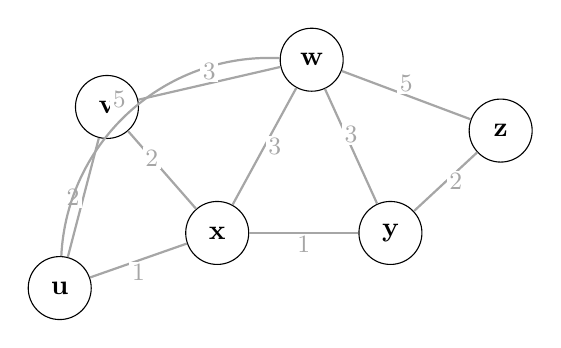
\begin{tikzpicture}[
    node/.style={circle, draw, minimum size=0.8cm, font=\bfseries},
    lbl/.style={font=\small, fill=white, inner sep=1pt},
    edge/.style={thick, gray!70}
]
    \node[node] (u) at (0,0)   {u};
    \node[node] (v) at (0.6,2.3) {v};
    \node[node] (w) at (3.2,2.9) {w};
    \node[node] (x) at (2.0,0.7) {x};
    \node[node] (y) at (4.2,0.7) {y};
    \node[node] (z) at (5.6,2.0) {z};

    \draw[edge] (u) -- node[lbl,left]{2} (v);
    \draw[edge] (u) -- node[lbl,below]{1} (x);
    \draw[edge] (u) to[bend left=45] node[lbl,above left]{5} (w);
    \draw[edge] (v) -- node[lbl,above]{3} (w);
    \draw[edge] (v) -- node[lbl,above left]{2} (x);
    \draw[edge] (w) -- node[lbl,right]{3} (x);
    \draw[edge] (w) -- node[lbl,above]{3} (y);
    \draw[edge] (w) -- node[lbl,above]{5} (z);
    \draw[edge] (x) -- node[lbl,below]{1} (y);
    \draw[edge] (y) -- node[lbl,right]{2} (z);
\end{tikzpicture}
\caption{链路状态算例拓扑：$u$ 为源，边上数字为链路代价}
\label{fig:ls_topo}
\end{figure}

从 $u$ 出发逐步执行，每轮选出一个节点加入 $N'$。表中 $D(\cdot)$ 写成「距离,前驱」的形式，\textbf{粗体}为该轮被选中的节点。

\begin{table}[H]
\centering
\caption{Dijkstra 从 $u$ 出发的逐步迭代表}
\renewcommand{\arraystretch}{1.35}
\small
\begin{tabulary}{\textwidth}{@{}c|C|C|C|C|C|C@{}}
\toprule
\textbf{轮} & \textbf{$N'$} & \textbf{$D(v)$} & \textbf{$D(w)$} & \textbf{$D(x)$} & \textbf{$D(y)$} & \textbf{$D(z)$} \\
\midrule
0 & $\{u\}$        & $2,u$ & $5,u$ & $\mathbf{1,u}$ & $\infty$ & $\infty$ \\
1 & $\{u,x\}$      & $2,u$ & $4,x$ & $1,u$          & $2,x$    & $\infty$ \\
2 & $\{u,x,v\}$    & $\mathbf{2,u}$ & $4,x$ & $1,u$ & $2,x$ & $\infty$ \\
3 & $\{u,x,v,y\}$  & $2,u$ & $4,x$ & $1,u$ & $\mathbf{2,x}$ & $4,y$ \\
4 & $\{u,x,v,y,w\}$& $2,u$ & $\mathbf{4,x}$ & $1,u$ & $2,x$ & $4,y$ \\
5 & 全部节点       & $2,u$ & $4,x$ & $1,u$ & $2,x$ & $\mathbf{4,y}$ \\
\bottomrule
\end{tabulary}
\end{table}

逐轮要点：
\begin{itemize}
    \item 第 0 轮：$u$ 的直接邻居为 $v,w,x$，距离分别为 $2,5,1$；$x$ 最小。
    \item 第 1 轮：加入 $x$ 后松弛其邻居——$w$ 由 $5$ 降为 $1+3=4$（前驱改 $x$），$y$ 由 $\infty$ 变 $1+1=2$。
    \item 第 2 轮：$v$ 的距离 $2$ 最小（与 $y$ 并列，约定任选其一），加入 $v$；经 $v$ 到 $w$ 为 $2+3=5>4$，不更新。
    \item 第 3 轮：加入 $y$，经 $y$ 到 $z$ 得 $2+2=4$。
    \item 第 4 轮：加入 $w$，经 $w$ 到 $z$ 为 $4+5=9>4$，不更新。
    \item 第 5 轮：最后加入 $z$，收敛。
\end{itemize}

于是 $u$ 到各目的的最小代价与下一跳为：

\begin{center}
$v:2$（经 $v$），$x:1$（经 $x$），$y:2$（经 $x$），$w:4$（经 $x$），$z:4$（经 $x$ $\to$ $y$）。
\end{center}

对应的最短路树如下（粗实线为树边，即每条路径的下一跳关系）。

\begin{figure}[H]
\centering
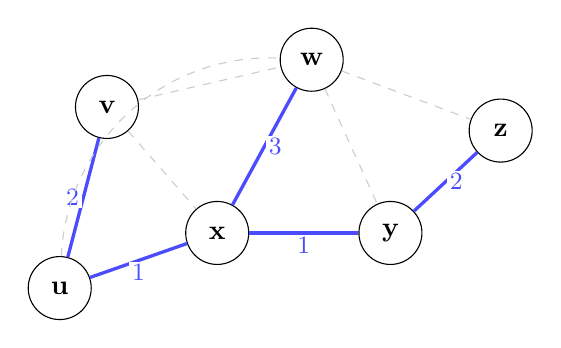
\begin{tikzpicture}[
    node/.style={circle, draw, minimum size=0.8cm, font=\bfseries},
    tree/.style={very thick, blue!70},
    lbl/.style={font=\small, fill=white, inner sep=1pt}
]
    \node[node] (u) at (0,0)   {u};
    \node[node] (v) at (0.6,2.3) {v};
    \node[node] (w) at (3.2,2.9) {w};
    \node[node] (x) at (2.0,0.7) {x};
    \node[node] (y) at (4.2,0.7) {y};
    \node[node] (z) at (5.6,2.0) {z};

    \draw[tree] (u) -- node[lbl,left]{2} (v);
    \draw[tree] (u) -- node[lbl,below]{1} (x);
    \draw[tree] (x) -- node[lbl,right]{3} (w);
    \draw[tree] (x) -- node[lbl,below]{1} (y);
    \draw[tree] (y) -- node[lbl,right]{2} (z);

    \draw[gray!40, dashed] (u) to[bend left=45] (w);
    \draw[gray!40, dashed] (v) -- (w);
    \draw[gray!40, dashed] (v) -- (x);
    \draw[gray!40, dashed] (w) -- (y);
    \draw[gray!40, dashed] (w) -- (z);
\end{tikzpicture}
\caption{以 $u$ 为根的最短路树：$u\to v$，$u\to x\to\{w,y\}$，$y\to z$}
\label{fig:ls_tree}
\end{figure}

\subsection{复杂度与讨论}

设 $|V|$ 个节点、$|E|$ 条链路。每轮需线性扫描未确定节点找最小 $D$，共 $|V|$ 轮，故朴素实现为
\begin{equation}
    T_{\text{naive}} = O\!\left(|V|^2\right).
\end{equation}
用二叉堆/斐波那契堆维护候选距离，可降为
\begin{equation}
    T_{\text{heap}} = O\!\left((|V|+|E|)\log|V|\right).
\end{equation}
LS 的代价是泛洪带来的开销 $O(|E|)$ 量级——每个节点都要把链路状态通告到全网。此外，若链路代价随负载动态变化，全网不同步地重算可能出现\textbf{路由振荡}：流量涌向「当前最便宜」的链路，反而把它压成最贵。缓解办法是让代价不直接正比于瞬时负载，或引入随机化。

\section{距离向量路由算法：Bellman--Ford}

\subsection{递推式与算法}

DV 算法基于动态规划：节点 $x$ 到目的 $y$ 的最短距离，等于「先花 $c(x,v)$ 走到某个邻居 $v$，再由 $v$ 走最短路到 $y$」在所有邻居中的最优值。这就是 \textbf{Bellman--Ford 方程}
\begin{equation}
    D_x(y) = \min_{v \in N(x)} \bigl\{\, c(x,v) + D_v(y) \,\bigr\},
    \label{eq:bf}
\end{equation}
其中 $N(x)$ 是 $x$ 的邻居集合。每个节点维护一个到全网各目的的距离向量 $D_x=[D_x(y)]_{y\in V}$，周期性或触发式地把自己的向量发给邻居。邻居拿到后用式 \eqref{eq:bf} 更新，若自身向量改变则继续通知其邻居。

\begin{algorithm}[H]
\caption{距离向量算法（在节点 $x$ 上运行）}
\begin{algorithmic}[1]
\Procedure{DV-Run}{$x$}
    \ForAll{目的 $y \in V$}
        \If{$y$ 是 $x$ 的邻居} $D_x(y)\gets c(x,y)$ \Else $D_x(y)\gets\infty$ \EndIf
    \EndFor
    \State 把向量 $D_x$ 发给所有邻居
    \Loop
        \State 等待：收到某邻居 $v$ 的向量 $D_v$，或本节点到某邻居的链路代价发生变化
        \ForAll{目的 $y \in V$}
            \State $D_x(y) \gets \min_{v\in N(x)} \bigl\{ c(x,v) + D_v(y) \bigr\}$ \Comment{按式 \eqref{eq:bf} 重算}
        \EndFor
        \If{$D_x$ 有任何分量改变} 把新向量 $D_x$ 发给所有邻居 \EndIf
    \EndLoop
\EndProcedure
\end{algorithmic}
\end{algorithm}

\subsection{好消息传得快}

当链路代价下降（好消息）时，DV 收敛很快。考虑简单的链 $x$--$y$--$z$，$c(x,y)=1$、$c(y,z)=1$。初始 $D_y(x)=1$，$D_z(x)=\infty$。若某时刻 $z$ 与 $x$ 直连的代价从 $\infty$ 降到 $2$：
\begin{itemize}
    \item $z$ 算出 $D_z(x)=\min(\infty,\,c(z,x)=2)=2$，通知 $y$；
    \item $y$ 算出 $D_y(x)=\min(c(y,z)+D_z(x),\,c(y,x),\,c(y,z)+D_z(x))=1+2=3$ 与直连 $1$ 比较取 $1$，其实不变；
    \item 若代价是\textbf{下降}（例如 $c(y,x)$ 由 $4$ 降到 $1$），$y$ 立即更新并把更小的 $D_y$ 广播出去，邻居再迅速改善。好消息一趟就能传遍，因为每一跳都在「下调」估计。
\end{itemize}

\subsection{坏消息传得慢：计数到无穷}

链路代价\textbf{上升}时情况截然不同。当节点发现经某邻居到达某目的地的路径其实绕回了自己，就会把错误的信息反复回传，估计值一轮一轮缓慢增大，称为\textbf{计数到无穷 (count to infinity)}。

取链 $x$--$y$--$z$，其中 $c(x,y)=4$、$c(y,z)=1$、$c(x,z)=50$。代价变化前达到的稳定态为
\begin{equation}
    D_y(x)=4 \;(\text{直连}), \qquad D_z(x)=\min(1+D_y(x),\,50)=5 \;(\text{经 }y).
\end{equation}
现在 $x$--$y$ 链路代价从 $4$ 骤升到 $60$（链路恶化）。$y$ 直接感知该变化，而 $z$ 尚未察觉。逐轮演算如下：

\begin{table}[H]
\centering
\caption{计数到无穷的逐步数值演算（$c(x,y):4\to 60$）}
\renewcommand{\arraystretch}{1.3}
\begin{tabulary}{\textwidth}{@{}c|C|C|L@{}}
\toprule
\textbf{轮次} & \textbf{$D_y(x)$} & \textbf{$D_z(x)$} & \textbf{说明} \\
\midrule
变化前 & $4$（直连） & $5$（经 $y$） & 稳定态 \\
1 & $6$（经 $z$） & $5$（经 $y$） & $y$: $\min(60,\,1+5)=6$ \\
2 & $6$ & $7$（经 $y$） & $z$: $\min(50,\,1+6)=7$ \\
3 & $8$（经 $z$） & $7$ & $y$: $\min(60,\,1+7)=8$ \\
4 & $8$ & $9$（经 $y$） & $z$: $\min(50,\,1+8)=9$ \\
5 & $10$（经 $z$） & $9$ & $y$: $\min(60,\,1+9)=10$ \\
$\vdots$ & $\vdots$ & $\vdots$ & 每轮各增 $2$，来回传播 \\
$k$ & $50$ & $49$ & $z$ 逼近其直连上限 $50$ \\
$k{+}1$ & $50$ & $50$ & $z$: $\min(50,\,1+50)=50$ \\
$k{+}2$ & $51$（经 $z$） & $50$ & 收敛：$y$ 走 $z$，$z$ 走直连 \\
\bottomrule
\end{tabulary}
\end{table}

要点：
\begin{itemize}
    \item $y$ 错误地以为「可以经 $z$ 到达 $x$」，而 $z$ 的路径恰恰又经过 $y$，形成\textbf{两节点路由环路}。
    \item 若 $x$--$z$ 之间根本不存在链路（$c(x,z)=\infty$），则 $D_y(x)$、$D_z(x)$ 会一直增大、永不收敛，这就是「计数到\emph{无穷}」的字面含义。
    \item 即使存在直连上限，收敛也要经历约 $(50-6)/2\approx 22$ 轮，期间分组可能在环中打转，响应极慢。
\end{itemize}

\subsection{缓解：水平分割与毒性逆转}

\textbf{水平分割 (split horizon)}：不把「到某目的地的距离」告诉通往该目的地的下一跳邻居，因为对方显然不该经由你到达该目的地。

\textbf{毒性逆转 (poisoned reverse)}：更强的版本——如果 $z$ 到 $x$ 的最短路是经 $y$ 的，那么 $z$ 通知 $y$ 时故意宣告 $D_z(x)=\infty$。在上例中，$z$ 会告诉 $y$「我无法到达 $x$」，于是 $y$ 不会误以为能经 $z$ 绕过去，两节点环路被立即切断。

毒性逆转并非万能：它只能消除两节点之间的环路，对于三节点及以上的环路仍可能失效。因此工程上常把 DV（如 RIP）限制在小规模网络，并配合较高的无穷大阈值、触发更新与抑制计时器。

\section{自治系统内部路由：OSPF}

现实互联网规模巨大，不可能让所有路由器运行同一个全局最短路。做法是把网络划分为若干\textbf{自治系统 (Autonomous System, AS)}，AS 内部使用\textbf{内部网关协议 (IGP)}，AS 之间使用\textbf{外部网关协议 (EGP)}。\textbf{OSPF (Open Shortest Path First)} 是应用最广的链路状态 IGP。

\subsection{机制与特性}

每个 OSPF 路由器泛洪链路状态通告，构建同一张拓扑图后运行 Dijkstra。相较朴素的 LS，OSPF 增加了多项工程能力：

\begin{itemize}
    \item \textbf{链路状态与 Dijkstra}：与前述链路状态算法原理一致，代价由管理员按带宽等设定。
    \item \textbf{分区域 (area)}：把 AS 再划分为若干区域以限制泛洪范围。一个特殊区域——\textbf{骨干区 (backbone area 0)}——连接所有其他区域。区域边界路由器 (ABR) 汇总区域间路由，自治系统边界路由器 (ASBR) 则与其他 AS 交换外部路由。分区域把链路状态通告的泛洪局部化，显著降低开销。
    \item \textbf{鉴别 (authentication)}：OSPF 报文可携带口令/MAC 鉴别，防止伪造的路由通告注入。
    \item \textbf{等代价多路径 (Equal-Cost Multi-Path, ECMP)}：当到同一目的存在多条等代价路径时，OSPF 可同时使用它们做负载分担，而非只保留一条。
    \item \textbf{快速收敛与可靠泛洪}：链路状态更新通过可靠机制传播，链路故障能被迅速检测并重新计算。
\end{itemize}

\begin{figure}[H]
\centering
\begin{tikzpicture}[
    rt/.style={circle, draw, minimum size=0.6cm, font=\small},
    abr/.style={circle, draw, fill=blue!15, minimum size=0.7cm, font=\small},
    lbl/.style={font=\small, align=center}
]
    \node[rt] (b1) at (0,0) {};
    \node[rt] (b2) at (1.4,0.6) {};
    \node[rt] (b3) at (1.4,-0.6) {};
    \node[abr] (ab1) at (3.0,0) {ABR};
    \draw (b1)--(b2); \draw (b1)--(b3); \draw (b2)--(ab1); \draw (b3)--(ab1);
    \node[lbl, above] at (1.0,0.9) {区域 0（骨干）};

    \node[rt] (a1) at (4.6,1.0) {};
    \node[rt] (a2) at (5.6,0.2) {};
    \node[rt] (a3) at (4.6,-1.0) {};
    \node[rt] (a4) at (5.6,-1.8) {};
    \draw (ab1)--(a1); \draw (a1)--(a2); \draw (ab1)--(a3); \draw (a3)--(a4); \draw (a2)--(a4);
    \node[lbl, align=center, anchor=west] at (6.1,-0.4) {区域 1\\(经 ABR 汇总)};

    \node[abr, fill=green!20] (asbr) at (-2.4,0) {ASBR};
    \draw (b1)--(asbr);
    \node[lbl, anchor=east] at (-2.9,0) {其他 AS};
\end{tikzpicture}
\caption{OSPF 层次结构：骨干区 0 汇聚各区域，ABR 汇总区域间路由，ASBR 连接外部 AS}
\label{fig:ospf_hier}
\end{figure}

OSPF 主要报文类型如下：

\begin{table}[H]
\centering
\caption{OSPF 五类报文}
\renewcommand{\arraystretch}{1.3}
\begin{tabulary}{\textwidth}{@{}CCL@{}}
\toprule
\textbf{类型} & \textbf{名称} & \textbf{用途} \\
\midrule
1 & Hello & 发现/维持邻居，选举指定路由器 \\
2 & Database Description & 交换链路状态数据库摘要 \\
3 & Link State Request & 请求缺失的链路状态通告 \\
4 & Link State Update & 泛洪链路状态通告（核心） \\
5 & Link State Ack & 确认收到通告，保证可靠泛洪 \\
\bottomrule
\end{tabulary}
\end{table}

\section{自治系统间路由：BGP}

AS 之间靠 \textbf{BGP (Border Gateway Protocol)} 交换可达性。与追求最短代价的 IGP 不同，BGP 的核心是\textbf{策略}：一个 AS 是否愿意为另一个 AS 转发流量，取决于商业关系（客户/提供商/对等），而非单纯的链路代价。因此 BGP 被称为互联网的「粘合剂」。

\subsection{路径向量与环路检测}

BGP 是一种\textbf{路径向量 (path-vector)} 协议：通告到某前缀时，携带\textbf{完整的 AS 路径}（如「$AS3 \to AS2 \to AS1$」），而不是仅仅一个距离。收到通告的路由器若发现路径中已包含本 AS，就知道会成环，直接丢弃——这天然实现了无环路由。路径向量是距离向量的推广：用「路径序列」替代「标量距离」，从而摆脱计数到无穷。

\subsection{eBGP 与 iBGP}

\begin{itemize}
    \item \textbf{eBGP (external BGP)}：运行在\textbf{不同 AS} 的边界路由器之间，跨越 AS 边界交换路由；
    \item \textbf{iBGP (internal BGP)}：运行在\textbf{同一 AS 内部}的路由器之间，把从 eBGP 学到的外部路由在 AS 内传播到所有需要它的路由器。
\end{itemize}

\begin{figure}[H]
\centering
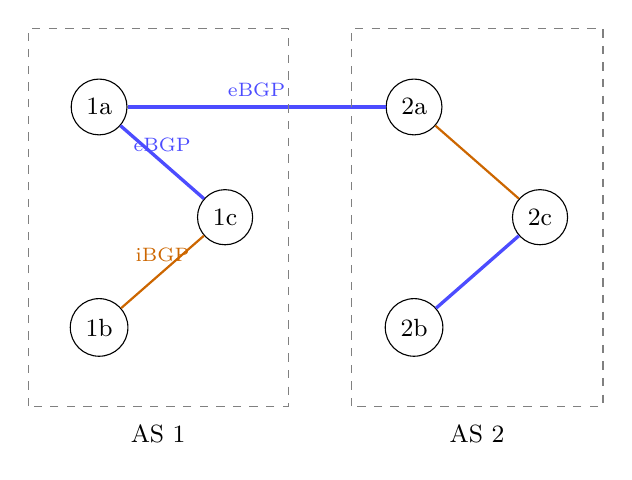
\begin{tikzpicture}[
    r/.style={circle, draw, minimum size=0.7cm, font=\small},
    lbl/.style={font=\small, align=center},
    e/.style={very thick, blue!70},
    i/.style={thick, orange!80!black}
]
    \node[r] (a1) at (0,1.4) {1a};
    \node[r] (a2) at (0,-1.4) {1b};
    \node[r] (a3) at (1.6,0) {1c};
    \draw[e] (a1)--(a3) node[midway, above, font=\scriptsize]{eBGP};
    \draw[i] (a2)--(a3) node[midway, above, font=\scriptsize]{iBGP};

    \node[r] (b1) at (4.0,1.4) {2a};
    \node[r] (b2) at (4.0,-1.4) {2b};
    \node[r] (b3) at (5.6,0) {2c};
    \draw[i] (b1)--(b3);
    \draw[e] (b2)--(b3);

    \draw[e] (a1) -- node[midway, above, font=\scriptsize]{eBGP} (b1);

    \draw[dashed, gray] (-0.9,-2.4) rectangle (2.4,2.4);
    \node[lbl] at (0.75,-2.75) {AS 1};
    \draw[dashed, gray] (3.2,-2.4) rectangle (6.4,2.4);
    \node[lbl] at (4.8,-2.75) {AS 2};
\end{tikzpicture}
\caption{eBGP 跨 AS 交换路由，iBGP 在 AS 内部分发（蓝色 eBGP，橙色 iBGP）}
\label{fig:bgp}
\end{figure}

\subsection{路径属性与选路决策}

BGP 通告携带多种\textbf{路径属性 (path attributes)}，它们是策略的载体：

\begin{table}[H]
\centering
\caption{BGP 常用路径属性}
\renewcommand{\arraystretch}{1.3}
\begin{tabulary}{\textwidth}{@{}CL@{}}
\toprule
\textbf{属性} & \textbf{含义} \\
\midrule
AS-PATH & 到达该前缀所经过的 AS 序列，用于环路检测与长度比较 \\
NEXT-HOP & 到达该前缀应交给的下一跳（边界路由器）地址 \\
LOCAL-PREF & 本地偏好，值越大越优先，用于表达「我更爱走这条出口」 \\
MED & 多出口鉴别器，向相邻 AS 建议入口偏好 \\
\bottomrule
\end{tabulary}
\end{table}

当同一前缀收到多条 BGP 路由时，路由器按以下（简化）顺序逐级比较，先满足者胜出：

\begin{enumerate}
    \item \textbf{本地偏好 LOCAL-PREF} 最高者优先（本地策略第一）；
    \item \textbf{AS 路径最短}：AS-PATH 中 AS 数最少；
    \item \textbf{热土豆路由 (hot potato routing)}：在仍打平的情况下，选择\textbf{本 AS 内到 NEXT-HOP 代价最小}（最近出口）的路由，尽快把分组「扔」出本 AS；
    \item 仍打平则用 BGP 标识符等做最终裁决。
\end{enumerate}

\textbf{热土豆路由}的直觉：本 AS 不关心分组出了本 AS 之后的命运，只求尽快、尽量省地把它交出去，代价就是 IGP 距离。它是典型的\textbf{策略路由}——最终路径未必是端到端最短，而是各 AS 各自决策的合成结果。

\section{ICMP：差错与控制报文}

IP 本身不可靠，也不报告错误。辅助它的是 \textbf{ICMP (Internet Control Message Protocol)}，它封装在 IP 数据报中（IPv4 协议号 1），用于传递差错与控制信息。ICMP 报文格式为：\textbf{类型 (type)} $+$ \textbf{代码 (code)} $+$ \textbf{检验和} $+$ 前 4 字节随类型而变 $+$ 可选数据区（通常携带触发该报文的原始 IP 首部及前 8 字节载荷，便于源端定位）。

\begin{table}[H]
\centering
\caption{常见 ICMP 报文类型}
\renewcommand{\arraystretch}{1.3}
\begin{tabulary}{\textwidth}{@{}CLC@{}}
\toprule
\textbf{类型} & \textbf{名称} & \textbf{典型用途} \\
\midrule
0 / 8 & 回显应答 / 回显请求 & \texttt{ping} 探测可达性与时延 \\
3 & 目的地不可达 & 网络/主机/端口不可达 \\
11 & 超时 & TTL 耗尽（\texttt{traceroute} 依赖） \\
5 & 重定向 & 提示更优的下一跳网关 \\
\bottomrule
\end{tabulary}
\end{table}

\subsection{\texttt{ping}}

若源主机周期性发送\textbf{回显请求 (type 8)}，目的主机回以\textbf{回显应答 (type 0)}。据此可测往返时间 (RTT) 与丢包率。注意许多主机会屏蔽 ICMP，因此「ping 不通」并不等价于「不可达」。

\subsection{\texttt{traceroute} 原理：TTL 递增}

\texttt{traceroute} 巧妙地利用 IP 首部的 \textbf{TTL} 字段与 ICMP 超时报文逐跳探测路径：

\begin{enumerate}
    \item 源主机依次发送一系列目的为同一目标、但 TTL $=1,2,3,\dots$ 的分组（通常用不可达的高端口 UDP 或 ICMP 回显请求）；
    \item TTL $=1$ 的分组到达第一跳路由器时 TTL 减为 $0$，被丢弃，路由器回送一个 \textbf{ICMP 超时 (type 11)} 报文，其中携带该路由器的地址；
    \item 源据此得知第 1 跳；随后 TTL $=2$ 的分组在第二跳耗尽，如此递推；
    \item 当分组终于到达目的主机时，目的端返回「端口不可达」(type 3, code 3) 或回显应答，探测结束。
\end{enumerate}

\begin{figure}[H]
\centering
\begin{tikzpicture}[
    h/.style={rectangle, draw, minimum width=1.0cm, minimum height=0.6cm, font=\small},
    arr/.style={-{Stealth[length=2.5mm]}, thick},
    lbl/.style={font=\scriptsize, align=center}
]
    \node[h] (s) at (0,0) {源};
    \node[h] (r1) at (2.6,0) {$R_1$};
    \node[h] (r2) at (5.2,0) {$R_2$};
    \node[h] (d) at (7.8,0) {目的};

    \draw[arr] (s.south) -- (r1.south) node[lbl, midway, below]{TTL$=1$ 耗尽};
    \draw[arr] (r1.north) to[bend left=40] node[lbl, above]{ICMP 超时} (s.north);
    \draw[arr] (s) -- (r2) node[lbl, midway, below, yshift=-1.4cm]{TTL$=2$};
    \draw[arr] (r2.north) to[bend left=55] node[lbl, above]{ICMP 超时} (s.north);
    \draw[arr] (s.south) to[bend right=8] (d.south) node[lbl, midway, below, yshift=-2.6cm]{TTL 足够大，到达目的};
    \draw[arr] (d.north) to[bend left=15] node[lbl, above]{端口不可达} (r2.north);
\end{tikzpicture}
\caption{\texttt{traceroute}：逐步增大 TTL，靠沿途 ICMP 超时报文勾出整条路径}
\label{fig:traceroute}
\end{figure}

\section{SDN：集中式控制平面}

传统路由器把控制平面（路由计算）和数据平面（转发）耦合在同一台设备内，每台各自运行分布式协议。\textbf{软件定义网络 (Software-Defined Networking, SDN)} 把二者解耦：控制平面集中到一台（或一簇）远程\textbf{控制器}，数据平面退化为通用、简单的\textbf{交换机}，只按控制器下发的规则做匹配与动作。

\subsection{OpenFlow：匹配$+$动作}

SDN 的南向接口以 \textbf{OpenFlow} 为代表。每台交换机的\textbf{流表 (flow table)} 由若干\textbf{流表项}组成，每项包含三部分：

\begin{itemize}
    \item \textbf{匹配字段 (match)}：对分组首部若干字段的匹配条件，可跨层组合，如入端口、源/目的 MAC、源/目的 IP、源/目的端口（TCP/UDP）、以及 VLAN、协议号等。支持通配（如 \texttt{10.0.0.*}）。
    \item \textbf{计数器 (counters)}：统计匹配到的分组数与字节数，供监控使用。
    \item \textbf{动作 (actions)}：匹配成功后执行的操作——\textbf{转发}到某端口、\textbf{丢弃}、\textbf{改写}（改 IP/端口）、或\textbf{送控制器}处理。
\end{itemize}

这一「\textbf{匹配$+$动作}」抽象统一了路由器、交换机、防火墙的功能：转发表、访问控制、NAT 都可用流表项表达。当分组与任何表项都不匹配时，交换机默认把它上送控制器，由控制器（全局视图下）决定下发新规则或直接处置。

\begin{table}[H]
\centering
\caption{OpenFlow 流表项示例}
\renewcommand{\arraystretch}{1.3}
\begin{tabulary}{\textwidth}{@{}LCC@{}}
\toprule
\textbf{匹配字段} & \textbf{动作} & \textbf{计数} \\
\midrule
入端口 $=1$, 目的 IP $=10.1.1.7$ & 转发端口 $3$ & 1240 包 \\
目的 IP $=10.2.0.0/16$ & 丢弃 & 87 包 \\
源 MAC $=\text{\texttt{00:..:A1}}$ & 送控制器 & 12 包 \\
\bottomrule
\end{tabulary}
\end{table}

\subsection{分层接口}

SDN 的架构常用三类接口描述：

\begin{itemize}
    \item \textbf{南向接口 (southbound)}：控制器 $\to$ 交换机，下发流表、查询状态，如 OpenFlow。
    \item \textbf{北向接口 (northbound)}：控制器 $\to$ 上层应用/编排系统，暴露抽象的网络视图与编程接口（如 REST）。路由、负载均衡、防火墙等应用在其上编程，而无需接触底层设备。
    \item \textbf{东向/西向接口}：多个控制器之间的横向通信，用于大规模网络下的控制平面扩展与一致。
\end{itemize}

\begin{figure}[H]
\centering
\begin{tikzpicture}[
    box/.style={draw, rounded corners, minimum width=2.1cm, minimum height=0.7cm, font=\small, align=center},
    arr/.style={{Stealth[length=2.5mm]}-{Stealth[length=2.5mm]}, thick}
]
    \node[box, fill=green!15] (app) at (0,2.6) {网络应用\\（路由/防火墙）};
    \node[box, fill=blue!15, minimum width=3.0cm] (ctrl) at (0,1.1) {SDN 控制器};
    \node[box] (s1) at (-3.2,-0.7) {交换机 1};
    \node[box] (s2) at (0,-0.7) {交换机 2};
    \node[box] (s3) at (3.2,-0.7) {交换机 3};

    \draw[arr] (app) -- (ctrl) node[midway, right, font=\scriptsize]{北向接口};
    \draw[arr] (ctrl) -- (s1) node[midway, left, font=\scriptsize]{南向};
    \draw[arr] (ctrl) -- (s2) node[midway, right, font=\scriptsize]{南向接口};
    \draw[arr] (ctrl) -- (s3) node[midway, right, font=\scriptsize]{南向};
\end{tikzpicture}
\caption{SDN 分层：应用经北向接口编程，控制器经南向接口（OpenFlow）下发流表}
\label{fig:sdn}
\end{figure}

\section{本章小结与常见误区}

\noindent\textbf{知识主线}：控制平面由\textbf{路由算法}计算转发表。\textbf{链路状态}算法让每个节点获得全网图，再用 \textbf{Dijkstra} 求最短路，工程化为 \textbf{OSPF}；\textbf{距离向量}算法让节点与邻居迭代交换向量，基于 \textbf{Bellman--Ford} 方程，典型协议是 RIP，其固有弱点是\textbf{计数到无穷}，需靠水平分割/毒性逆转缓解。跨 AS 的路由由 \textbf{BGP} 承担，它是\textbf{路径向量}协议，强调\textbf{策略}而非最短，eBGP 跨域、iBGP 域内传播。\textbf{ICMP} 承载差错与控制报文，是 \texttt{ping} 与 \texttt{traceroute} 的基础。\textbf{SDN} 把控制平面集中到控制器，用 OpenFlow 的「匹配$+$动作」流表统一转发。

常见误区：

\begin{itemize}
    \item \textbf{「路由算法一定求最短路径」}：BGP 的目标是策略与可达性，最终路径常常并非端到端最短；热土豆路由就是「只求尽快出本 AS」。
    \item \textbf{「Dijkstra 的 $D(v)$ 就是最终最短路」}：在被选入 $N'$ 之前，$D(v)$ 只是上界估计；只有加入 $N'$ 时才确定。
    \item \textbf{「DV 一定能收敛到正确值」}：坏消息下可能出现计数到无穷；若网络无直连替代路径且无缓解机制，估计值会无限增大。
    \item \textbf{「毒性逆转能彻底解决环路」}：它只切断两节点环路，长度 $\ge 3$ 的环路仍可能存在。
    \item \textbf{「iBGP 是另一种协议」}：iBGP 与 eBGP 同属 BGP，区别只在会话两端是否处于同一 AS。
    \item \textbf{「ping 不通说明主机离线」}：ICMP 常被防火墙屏蔽，「不通」只说明没有回显应答。
    \item \textbf{「SDN 就是 OpenFlow」}：OpenFlow 只是主流南向协议之一；SDN 的本质是控制平面与数据平面\textbf{解耦}与集中控制。
    \item \textbf{「链路状态泛洪没有代价」}：泛洪是 $O(|E|)$ 量级的全网开销，OSPF 的分区域正是为限制它。
\end{itemize}

\clearpage
\clearpage
\begingroup
\let\clearpage\relax
\let\cleardoublepage\relax
\vspace*{\fill}
\chapter{链路层与局域网}
\begin{center}
链路层负责在「直接相连的节点」之间搬运数据帧，是网络层数据报真正落到物理介质上的最后一跳。
本章从链路层的服务与实现位置讲起，依次展开差错检测、多路访问、ARP、以太网与交换机、VLAN，
并给出可手算的例题与常见误区，力求让读者能独立完成 CRC 长除、ALOHA 效率推导与交换机自学习表的填写。
\end{center}
\vspace*{\fill}
\endgroup
\clearpage

\section{链路层服务与实现位置}

\subsection{动机：为什么需要链路层}

网络层把数据报从源主机送到目的主机，靠的是路由器之间的逐跳转发。
但「一跳」究竟如何把一串比特从一台设备送到\textbf{物理上直接相连}的另一台设备？
这正是链路层 (link layer) 要解决的问题。链路层运行在每一台主机和每一台路由器上，
把网络层交下来的数据报封装成\textbf{帧 (frame)}，通过一条具体的链路（有线、无线、交换式以太网、Wi-Fi 等）传送到相邻节点。

所谓「直接相连」，可以是通过一根点对点链路相连，也可以是通过一个共享的广播介质（如早期的同轴电缆或无线信道）相连。
不同介质的链路层协议差别很大，但它们都提供一组共同的核心服务。

\subsection{链路层提供的服务}

\begin{itemize}
    \item \textbf{成帧 (framing)}：把网络层数据报封装进帧，加上首部与尾部。
        首部通常含源/目的 MAC 地址，尾部含差错检测码。帧的边界靠前导码、长度字段或特殊定界符来确定。
    \item \textbf{链路接入 (link access)}：当多个节点共享同一介质时，由 \textbf{MAC 协议}（介质访问控制协议）决定「谁可以在这条链路上发送」。
        点对点链路（如 PPP）无需竞争；广播链路（如以太网、Wi-Fi）必须仲裁。
    \item \textbf{可靠交付 (reliable delivery)}：在误码率高的链路上（典型是无线），链路层可在本地做「确认 + 重传」，
        把差错尽量在本地修复，避免端到端重传。对于低误码率的有线链路（如光纤、双绞线），通常不做可靠交付，交由运输层负责。
    \item \textbf{差错检测与纠正 (error detection / correction)}：链路层在帧中附加冗余比特，接收方据此判断帧是否出错，
        发现错误一般直接丢弃（偶尔可纠正）。常见方法有位/二维奇偶校验、因特网检验和、CRC。
\end{itemize}

\begin{table}[H]
\centering
\caption{不同链路的链路层服务取舍}
\begin{tabulary}{\textwidth}{@{}LCC@{}}
\toprule
\textbf{服务} & \textbf{点对点/有线链路} & \textbf{广播/无线链路} \\
\midrule
成帧 & 需要 & 需要 \\
链路接入 & 简单（几乎独占） & 复杂（需竞争仲裁） \\
可靠交付 & 通常不做（误码低） & 常做（误码高，本地重传） \\
差错检测 & 需要（CRC） & 需要（CRC + 确认重传） \\
\bottomrule
\end{tabulary}
\end{table}

\subsection{实现位置：网卡、驱动与硬件}

链路层的一个关键特点是：它\textbf{主要用硬件实现}。承载链路层功能的部件叫\textbf{网络适配器 (network adapter)}，俗称\textbf{网卡 (NIC)}。
网卡内部集成了链路层控制器（专用芯片），并实现物理层与链路层的功能。

\begin{figure}[H]
\centering
\begin{tikzpicture}[font=\small,
    box/.style={draw, rounded corners, minimum width=3.4cm, minimum height=0.75cm, align=center},
    hw/.style={draw, fill=blue!8, rounded corners, minimum width=3.4cm, minimum height=0.75cm, align=center},
    arrow/.style={->, >=latex, thick}
]
    \node[box] (app) at (0,3.6) {应用层 / 运输层 / 网络层};
    \node[box] (drv) at (0,2.4) {设备驱动程序 (driver)};
    \node[hw]  (nic) at (0,1.2) {网络适配器（网卡 NIC）};
    \node[hw]  (phy) at (0,0.0) {物理介质接口（PHY）};
    \node[box] (bus) at (-4.6,2.4) {主机总线 (PCIe)};

    \draw[arrow] (app) -- (drv);
    \draw[arrow] (drv) -- (nic);
    \draw[arrow] (nic) -- (phy);
    \draw[arrow] (bus.east) -- (drv.west);
    \node[font=\small, anchor=west, align=left] at (2.2,1.2) {链路层核心逻辑\\在硬件中完成};
    \node[font=\small, anchor=west, align=left] at (2.2,2.4) {驱动负责在\\主机与网卡间搬运帧};
\end{tikzpicture}
\caption{链路层的实现位置：网络层以上是软件，链路层主体在网卡硬件中}
\label{fig:nic_location}
\end{figure}

由此得到一个重要结论：\textbf{链路层的大部分逻辑运行在网卡上}。
当主机收到一个帧时，网卡先做差错检测，若无错则把帧交给驱动，再由驱动交给网络层；
若出错则直接丢弃，不会打扰 CPU。这也解释了为什么链路层协议在不同硬件上实现各异。

\section{差错检测}

\subsection{一位奇偶校验}

最简单的方法是在数据后附加 \textbf{1 个奇偶校验位 (parity bit)}，使整个码字中「\texttt{1}」的个数满足约定：

\begin{itemize}
    \item \textbf{偶校验}：让「\texttt{1}」的总个数为偶数。
    \item \textbf{奇校验}：让「\texttt{1}」的总个数为奇数。
\end{itemize}

例如数据 \texttt{1011010} 中有 $4$ 个 \texttt{1}（偶数），若采用奇校验则校验位取 \texttt{1}，发送 \texttt{10110101}；
若采用偶校验则校验位取 \texttt{0}。接收方统计 \texttt{1} 的个数即可判断奇偶性。

\textbf{局限}：一位奇偶校验只能检测\textbf{奇数个}比特错误。若同时翻转 2 个比特，\texttt{1} 的个数奇偶性不变，错误就被漏检了。

\subsection{二维奇偶校验}

把数据排成 $m$ 行 $n$ 列的矩阵，对每一行、每一列各加一个校验位，形成二维校验码。
接收方既检查每行也检查每列，可以\textbf{定位并纠正}单个比特错误；若两个比特出错，通常也能检测到（但无法纠正）。

\begin{figure}[H]
\centering
\begin{tikzpicture}[font=\ttfamily\small,
    cell/.style={draw, minimum size=0.7cm},
    pcell/.style={draw, minimum size=0.7cm, fill=green!12},
    hd/.style={font=\small\sffamily}
]
    \matrix (m) [matrix of nodes, nodes={cell}, column sep=-\pgflinewidth, row sep=-\pgflinewidth,
        row 4/.style={nodes={pcell}},
        column 5/.style={nodes={pcell}}]{
        1 & 0 & 1 & 1 & 1 \\
        0 & 1 & 1 & 0 & 0 \\
        1 & 1 & 0 & 0 & 0 \\
        0 & 0 & 0 & 1 & 1 \\
    };
    \node[hd, above=0.15cm of m.north] {行校验位（第 5 列）};
    \node[hd, anchor=west] at ($(m.east)+(0.25,0)$) {列校验位（第 4 行）};
\end{tikzpicture}
\caption{二维奇偶校验：行、列各加校验位，可定位单个比特错误}
\label{fig:2d_parity}
\end{figure}

\subsection{因特网检验和 (Internet Checksum)}

因特网检验和用于 IP、TCP、UDP 首部（及其数据）的差错检测。算法如下：

\begin{enumerate}
    \item 把数据看成若干 \textbf{16 位字}，逐字相加（\textbf{反码求和}）；
    \item 若最高位产生进位，把进位\textbf{回卷}到最低位（end-around carry）；
    \item 对最终和取\textbf{反码 (1 的补码)}，即得检验和。
\end{enumerate}

接收方把包括检验和在内的所有 16 位字相加再取反，结果应为全 \texttt{0}（即 $1111\cdots1111$ 的反码），否则判为出错。

\noindent\textbf{算例}：设两个 16 位字为
\[
w_1 = \texttt{0110011001100110},\qquad w_2 = \texttt{0101010101010101}.
\]
反码求和：
\[
\begin{array}{r@{\;}l}
  & \texttt{0110\,0110\,0110\,0110}\\
+ & \texttt{0101\,0101\,0101\,0101}\\
\hline
  & \texttt{1011\,1011\,1011\,1011}
\end{array}
\]
无进位，直接取反码得检验和
\[
\text{checksum} = \texttt{0100\,0100\,0100\,0100}.
\]
发送方把 $w_1,w_2$ 与该检验和一起发出；接收方三者相加应得 \texttt{1111\,1111\,1111\,1111}。

\noindent\textbf{易错点}：检验和只做加法，强度远弱于 CRC，但它实现极简单，软件中一次循环即可完成，
因此适合在协议栈软件中计算；而 CRC 由网卡硬件计算，速度极快。

\subsection{循环冗余校验 (CRC)}

\textbf{CRC (Cyclic Redundancy Check)} 是链路层最常用的检错方法，由硬件实现。
把发送的数据 $D$（$d$ 位）视为一个二进制多项式，选定一个 $r+1$ 位的\textbf{生成多项式 (generator)} $G$。
发送方用模 2 除法（异或，不借位）计算余数 $R$（$r$ 位），并把 $R$ 附在数据后发送：

\begin{equation}
    D \cdot 2^{r} \;\text{xor}\; R \;=\; nG \quad(\text{即结果可被 } G \text{ 整除})
    \label{eq:crc}
\end{equation}

\begin{figure}[H]
\centering
\begin{tikzpicture}[font=\small, align=center]
    \draw (0,0) rectangle (4,0.7) node[midway]{数据 $D$（$d$ 位）};
    \draw (4,0) rectangle (5.3,0.7) node[midway]{$R$（$r$ 位）};
    \node[anchor=west] at (5.5,0.35) {$\to$ 发送的码字};
    \draw[decorate, decoration={brace, amplitude=5pt, mirror}] (0,-0.05) -- (5.3,-0.05)
        node[midway, below=6pt]{发送码字共 $d+r$ 位};
\end{tikzpicture}
\caption{CRC 帧结构：原始数据拼接 $r$ 位余数}
\label{fig:crc_frame}
\end{figure}

\subsubsection{完整长除例题}

取数据 $D=\texttt{101110}$，生成多项式 $G=\texttt{1001}$。
$G$ 有 $4$ 位，故 $r=3$，需在 $D$ 后补 $3$ 个 \texttt{0} 得到被除数
\[
D\cdot 2^{3} = \texttt{101110000}.
\]
逐步模 2 长除（每位只看当前余数的最高位，为 \texttt{1} 则与 $G$ 异或）：

\begin{align*}
&\texttt{101110000} \div \texttt{1001}\\[2pt]
\text{第 1 步: } & \texttt{1011} \oplus \texttt{1001} = \texttt{0010},\ \text{落下下一位得 }\texttt{0101}\\
\text{第 2 步: } & \texttt{0101} \text{ 最高位为 0，仅落下一位得 }\texttt{1010}\\
\text{第 3 步: } & \texttt{1010} \oplus \texttt{1001} = \texttt{0011},\ \text{落下一位得 }\texttt{0110}\\
\text{第 4 步: } & \texttt{0110} \text{ 最高位为 0，落下一位得 }\texttt{1100}\\
\text{第 5 步: } & \texttt{1100} \oplus \texttt{1001} = \texttt{0101},\ \text{落下一位得 }\texttt{1010}\\
\text{第 6 步: } & \texttt{1010} \oplus \texttt{1001} = \texttt{0011}
\end{align*}

最终余数（取低 $r=3$ 位）为
\[
R = \texttt{011}.
\]
于是发送码字为
\[
D\cdot 2^{3} \oplus R = \texttt{101110000} \oplus \texttt{000000011} = \texttt{101110011}.
\]

\noindent\textbf{验证}：接收方用同一个 $G=\texttt{1001}$ 去除收到的 \texttt{101110011}，若余数为 \texttt{000} 则认为无错。
用移位寄存器手算（寄存器 3 位，初值 \texttt{000}，逐位「左移入位，最高位为 1 则异或 \texttt{001}」）：

\begin{center}
\begin{tabular}{cccccccccc}
\toprule
输入位 & \texttt{1} & \texttt{0} & \texttt{1} & \texttt{1} & \texttt{1} & \texttt{0} & \texttt{0} & \texttt{1} & \texttt{1}\\
\midrule
寄存器 & \texttt{001} & \texttt{010} & \texttt{101} & \texttt{010} & \texttt{101} & \texttt{011} & \texttt{110} & \texttt{100} & \texttt{000}\\
\bottomrule
\end{tabular}
\end{center}
末态寄存器为 \texttt{000}，说明码字能被 $G$ 整除，与式~\eqref{eq:crc} 一致。

\subsubsection{CRC 的检错能力}

\begin{itemize}
    \item 若 $G$ 含有因子 $(x+1)$，则 CRC 能检测\textbf{所有奇数个}比特错误（因为奇数个错误对应的多项式在 $x=1$ 处不为零）。
    \item 只要 $G$ 的位数足够，CRC 可检测所有\textbf{长度不超过 $r$ 位}的突发错误。
    \item 对长度超过 $r$ 的突发错误，漏检概率约为 $2^{-r}$。工程上取 $r=32$（如 CRC-32）时，漏检概率极低。
    \item 与奇偶校验、检验和相比，CRC 用同样甚至更少的冗余位，却能检测更广泛的错误模式，且完全由硬件并行实现。
\end{itemize}

\section{多路访问协议}

当多个节点共享同一条广播信道时，如果两个节点同时发送，信号会\textbf{叠加冲突 (collision)}，接收方无法正确解析。
\textbf{多路访问协议 (multiple access protocol)} 就是用来协调各节点发送的规则，可分为三大类。

\begin{table}[H]
\centering
\caption{三类多路访问协议}
\begin{tabulary}{\textwidth}{@{}LCC@{}}
\toprule
\textbf{类型} & \textbf{基本思想} & \textbf{代表协议} \\
\midrule
信道划分 & 把信道在时间/频率/码域上静态切分给各节点 & TDMA / FDMA / CDMA \\
随机接入 & 不划分，节点随机发送，冲突后重试 & ALOHA / CSMA / CSMA/CD \\
轮流 & 节点按某种次序轮流获得发送权 & 轮询 / 令牌环 \\
\bottomrule
\end{tabulary}
\end{table}

\subsection{信道划分协议}

\begin{itemize}
    \item \textbf{TDMA（时分多址）}：时间被划分为时隙，每个节点固定分配一个时隙发送。
        优点是无冲突；缺点是节点空闲时时隙浪费，且需时间同步。
    \item \textbf{FDMA（频分多址）}：把频带划分为若干子频带，每个节点固定使用一个子频带。
        同样无冲突，但节点空闲时频段浪费。
    \item \textbf{CDMA（码分多址）}：所有节点同时同频发送，但各自用不同的\textbf{正交码}对信号编码。
        接收方用对应的码做相关运算即可分离出目标信号，抗干扰强，广泛用于 3G 等无线系统。
\end{itemize}

信道划分的共性缺点是：当节点数少、流量突发时，固定分配会浪费大量信道容量。

\subsection{随机接入协议}

\subsubsection{纯 ALOHA 及其效率}

纯 ALOHA 的规则最简单：节点有帧就立即发送；若发生冲突，则等待一段随机时间后重发。
设帧长为 $1$ 个时间单位，所有节点产生新帧加上重传帧的\textbf{总到达率}为 $G$（每帧时内的帧数），
则单个节点成功发送的概率等于「在发送该帧的一个帧时内，前后各一个帧时都无人发送」的概率：

\begin{equation}
    P_{\text{成功}} = e^{-G}\cdot e^{-G} = e^{-2G}.
\end{equation}
故吞吐量为
\begin{equation}
    S(G) = G\,e^{-2G}.
\end{equation}
对 $G$ 求导并令其为零：
\[
\frac{dS}{dG} = e^{-2G}(1-2G) = 0 \;\Rightarrow\; G = \tfrac{1}{2}.
\]
代回得最大吞吐量
\begin{equation}
    S_{\max} = \tfrac{1}{2}\,e^{-2\cdot\frac12} = \frac{1}{2e} \approx 0.184.
    \label{eq:aloha_pure}
\end{equation}
即纯 ALOHA 最多只能利用信道容量的约 $18.4\%$。

\subsubsection{时隙 ALOHA 及其效率}

时隙 ALOHA 把时间划分为等长时隙，节点只能在\textbf{时隙边界}开始发送，冲突只可能发生在同一时隙内。
此时只需保证「该时隙内没有其他节点发送」，成功概率为 $e^{-G}$，故

\begin{equation}
    S(G) = G\,e^{-G}.
\end{equation}
求导：$\frac{dS}{dG} = e^{-G}(1-G)=0 \Rightarrow G=1$，于是
\begin{equation}
    S_{\max} = 1\cdot e^{-1} = \frac{1}{e} \approx 0.368.
    \label{eq:aloha_slotted}
\end{equation}
时隙化把效率提高了一倍，代价是需要全网时间同步。

\begin{figure}[H]
\centering
\begin{tikzpicture}[font=\small, x=1.4cm, y=1cm]
    \draw[->] (0,0) -- (6.2,0) node[right]{$G$};
    \draw[->] (0,0) -- (0,1.6) node[above]{$S$};
    \draw[thick, blue, domain=0.02:6, samples=120] plot (\x, {\x*exp(-\x)});
    \draw[thick, red, domain=0.02:6, samples=120] plot (\x, {\x*exp(-2*\x)});
    \draw[dashed] (1,0) -- (1,0.368) -- (0,0.368);
    \node[blue, anchor=west] at (3.2,1.15) {时隙 ALOHA: $Ge^{-G}$};
    \node[red, anchor=west] at (3.2,0.55) {纯 ALOHA: $Ge^{-2G}$};
    \node[font=\tiny, blue, anchor=south] at (1,0.368) {$\frac{1}{e}$};
    \node[font=\tiny, red, anchor=west] at (1.6,0.12) {$\frac{1}{2e}$};
\end{tikzpicture}
\caption{两种 ALOHA 的吞吐量 $S$ 随负载 $G$ 的变化}
\label{fig:aloha_curves}
\end{figure}

\subsubsection{CSMA 与 CSMA/CD}

ALOHA 的致命弱点是「不等信道空闲就发」。\textbf{载波监听多路访问 (CSMA)} 要求节点\textbf{发送前先监听信道}：
\begin{itemize}
    \item \textbf{1-坚持 CSMA}：信道忙则持续监听，一空闲立即发送（冲突概率高）。
    \item \textbf{非坚持 CSMA}：信道忙则随机等待一段时间再监听（减少冲突但增加空闲时间）。
    \item \textbf{p-坚持 CSMA}：信道空闲时以概率 $p$ 发送，以 $1-p$ 推迟到下一时隙。
\end{itemize}

即使监听了，由于\textbf{传播时延}，两个节点可能几乎同时判定「信道空闲」而同时发送，仍会冲突。
\textbf{CSMA/CD (Collision Detection)} 在 CSMA 基础上增加\textbf{冲突检测}：边发边听，一旦检测到冲突立即停止发送，
发送一个\textbf{干扰信号 (jam signal)} 通知全网，然后进入退避。

\begin{figure}[H]
\centering
\begin{tikzpicture}[font=\small, align=center,
    node distance=0.6cm,
    blk/.style={draw, rounded corners, minimum width=2.7cm, minimum height=0.6cm, align=center},
    arrow/.style={->, >=latex, thick}
]
    \node[blk] (a) {载波监听\\信道空闲？};
    \node[blk, right=1.2cm of a] (b) {发送帧};
    \node[blk, right=1.2cm of b] (c) {检测到冲突？};
    \node[blk, below=0.9cm of c] (d) {发送 jam 信号\\执行二进制指数退避};
    \draw[arrow] (a) -- node[above]{空闲} (b);
    \draw[arrow] (b) -- (c);
    \draw[arrow] (c) -- node[right]{是} (d);
    \draw[arrow] (d) -| (a);
    \draw[arrow] (c.east) -- ++(1.0,0) node[above, font=\tiny, align=center]{否，\\发送完成};
\end{tikzpicture}
\caption{CSMA/CD 的发送流程}
\label{fig:csmacd_flow}
\end{figure}

\subsubsection{二进制指数退避（含例题）}

发生第 $m$ 次冲突后，节点从集合
\[
\{0,1,2,\dots,2^{m}-1\}
\]
中随机取一个整数 $K$，等待 $K \cdot 512$ 比特时间（以太网中 $512$ 比特时间 $=51.2\,\mu s$，即一个\textbf{时隙}）。
冲突次数越多，退避窗口越大，网络越拥挤时等待越久。当 $m>10$ 时窗口固定为 $\{0,\dots,1023\}$，当 $m>16$ 则放弃并报错。

\noindent\textbf{例题}：某节点连续发生了 3 次冲突。求其本次可选的退避窗口、等待 $K=4$ 的概率以及对应的等待时间。

\noindent\textbf{解}：第 3 次冲突，$m=3$，窗口为 $\{0,1,\dots,2^3-1\}=\{0,1,2,3,4,5,6,7\}$，共 $8$ 个取值。
若各值等概率，则
\[
P(K=4) = \frac{1}{8} = 12.5\%.
\]
对应等待时间为
\[
K\cdot 512 = 4\times 512 = 2048\ \text{比特时间} = 2048 \times 0.1\,\mu s = 204.8\,\mu s.
\]
（在 $10$ Mbps 以太网中，$1$ 比特时间 $=0.1\,\mu s$。）

\subsection{轮流协议}

\begin{itemize}
    \item \textbf{轮询 (polling)}：设一个主节点，依次询问各从节点是否有数据发送。无冲突、可按需分配，
        但引入轮询时延，且主节点是单点故障。
    \item \textbf{令牌环 (token ring)}：一个称为\textbf{令牌}的特殊帧在环上循环，只有持有令牌的节点才能发送。
        无冲突且高负载下效率高，但令牌丢失或节点故障需要复杂的恢复机制。
\end{itemize}

\section{ARP：地址解析协议}

\subsection{为什么需要 ARP}

网络层用 \textbf{IP 地址}标识主机，链路层用 \textbf{MAC 地址}标识网卡。当主机要发送 IP 数据报时，
它知道下一跳的 IP 地址，但网卡真正要填入帧首部的是下一跳的 \textbf{MAC 地址}。
\textbf{ARP (Address Resolution Protocol)} 就是完成「IP 地址 $\to$ MAC 地址」映射的协议。

\subsection{同一子网内的解析流程}

假设主机 A（IP \texttt{192.168.1.1}，MAC \texttt{AA}）要向同子网的主机 B（IP \texttt{192.168.1.2}，MAC \texttt{BB}）发送数据：

\begin{enumerate}
    \item A 先查自己的 \textbf{ARP 缓存}，若已有 B 的映射则直接使用。
    \item 若没有，A 构造 \textbf{ARP 请求}：「谁是 \texttt{192.168.1.2}？请告诉 \texttt{192.168.1.1}」，
        以\textbf{广播} MAC 地址 \texttt{FF:FF:FF:FF:FF:FF} 发出。
    \item 子网内所有主机都收到该请求，但只有 IP 匹配的 B 会响应。
    \item B 以\textbf{单播} \textbf{ARP 应答}回复 A，携带自己的 MAC \texttt{BB}。
    \item A 收到应答后，把映射 $(\texttt{192.168.1.2} \to \texttt{BB})$ 写入 ARP 缓存（带 TTL，通常 $20$ 分钟），随后发送数据帧。
\end{enumerate}

\begin{figure}[H]
\centering
\begin{tikzpicture}[font=\small, align=center,
    host/.style={draw, rounded corners, minimum width=2.6cm, minimum height=0.9cm, align=center},
    arrow/.style={->, >=latex, thick}
]
    \node[host] (a) at (0,0) {A\\\texttt{192.168.1.1 / AA}};
    \node[host] (b) at (6,0) {B\\\texttt{192.168.1.2 / BB}};
    \draw[arrow] ($(a.east)+(0,0.25)$) -- node[above, font=\small]{ARP 请求（广播）} ($(b.west)+(0,0.25)$);
    \draw[arrow] ($(b.west)-(0,0.25)$) -- node[below, font=\small]{ARP 应答（单播 \texttt{BB}）} ($(a.east)-(0,0.25)$);
\end{tikzpicture}
\caption{同子网 ARP：广播请求，单播应答}
\label{fig:arp_same_subnet}
\end{figure}

\subsection{跨子网：经网关}

若目的主机不在同一子网，A 无法直接解析到目的 MAC。此时 A 把\textbf{默认网关（路由器接口）}的 IP 解析为 MAC，
把帧的目的 MAC 填成网关的 MAC，而 IP 数据报中的目的 IP 仍是最终主机。
路由器收到后剥离链路层帧，按路由表查下一跳，再在其出口子网中重新用 ARP 解析下一跳的 MAC。
也就是说：\textbf{MAC 地址逐跳改变，IP 地址端到端不变}。

\noindent\textbf{易错点}：ARP 请求是广播，ARP 应答是单播；ARP 只在同一子网内使用；
一台主机的 ARP 缓存可能被伪造应答污染（ARP 欺骗），需靠静态绑定或 DAI 等机制防护。

\section{以太网}

\subsection{MAC 地址}

以太网的链路层地址是 \textbf{MAC 地址}，长 \textbf{48 位}（6 字节），通常写成
\texttt{1A:2B:3C:4D:5E:6F}。其中前 24 位是厂商 OUI，后 24 位由厂商分配。
\texttt{FF:FF:FF:FF:FF:FF} 是广播地址。MAC 地址\textbf{扁平、不具层次}，与位置无关，
因此离开本子网后需要靠 ARP 重新解析。

\subsection{以太网帧格式}

\begin{figure}[H]
\centering
\begin{tikzpicture}[font=\small, align=center]
    \def\w{1.5}
    \draw (0,0) rectangle (\w,0.8) node[midway, align=center]{前导码\\8 B};
    \draw (\w,0) rectangle (2*\w,0.8) node[midway, align=center]{目的\\MAC 6 B};
    \draw (2*\w,0) rectangle (3*\w,0.8) node[midway, align=center]{源\\MAC 6 B};
    \draw (3*\w,0) rectangle (4*\w,0.8) node[midway, align=center]{类型\\2 B};
    \draw (4*\w,0) rectangle (6.2*\w,0.8) node[midway, align=center]{数据 (载荷)\\46--1500 B};
    \draw (6.2*\w,0) rectangle (7.2*\w,0.8) node[midway, align=center]{CRC\\4 B};
    \node[anchor=west, font=\small] at (7.3*\w,0.4) {$\to$ 时间顺序};
\end{tikzpicture}
\caption{DIX 以太网帧格式（前导码不计入帧长）}
\label{fig:eth_frame}
\end{figure}

逐字段说明：

\begin{itemize}
    \item \textbf{前导码 (Preamble, 8 B)}：前 7 字节 \texttt{10101010} 用于收发双方时钟同步，第 8 字节 \texttt{10101011} 是帧起始定界符 (SFD)。
    \item \textbf{目的 MAC (6 B)}：接收网卡据此判断是否接收（匹配本机、广播或组播）。
    \item \textbf{源 MAC (6 B)}：发送网卡的地址。
    \item \textbf{类型 (Type, 2 B)}：指出上层协议，如 \texttt{0x0800} 表示 IPv4、\texttt{0x0806} 表示 ARP、\texttt{0x8100} 表示 802.1Q VLAN。
    \item \textbf{数据 (46--1500 B)}：承载上层数据报。若不足 46 B 需填充到 46 B；1500 B 是以太网的 \textbf{MTU}。
    \item \textbf{CRC (4 B)}：帧校验序列，用于检错，出错即丢弃。
\end{itemize}

以太网是\textbf{无连接、不可靠}的：发送前不握手，收到坏帧直接丢弃，不发送确认也不重传。

\subsection{最小帧 64 字节的原因}

以太网规定从目的 MAC 到 CRC 至少 $6+6+2+46+4 = 64$ 字节（前导码不计入）。
原因是 \textbf{CSMA/CD 必须保证发送方在帧发送完毕之前能检测到冲突}。
设最远两台主机间的往返传播时延为 $2\tau$，则发送方至少要持续发送 $2\tau$ 时间才能确保听到最远处产生的冲突。
定义\textbf{时隙}为 $2\tau = 51.2\,\mu s$，在 $10$ Mbps 下对应 $512$ 比特 $=64$ 字节。
因此帧长不得小于 64 字节，否则可能在检测到冲突前就已发完，误以为发送成功。
若数据不足 46 字节，靠填充凑够最小帧。

\subsection{链路层交换机与自学习}

\textbf{交换机 (switch)} 是工作在链路层的设备，每个端口是一个独立的碰撞域，采用全双工则完全无碰撞。
交换机维护一张\textbf{转发表 (forwarding table)}，表项为 $(\text{MAC 地址}, \text{端口}, \text{老化时间})$，
并通过\textbf{自学习}自动建立。

\subsubsection{自学习算法}

\begin{enumerate}
    \item 收到帧时，记录其\textbf{源 MAC} 与\textbf{入端口}，更新转发表（覆盖旧表项，重置老化计时）。
    \item 查目的 MAC：
    \begin{itemize}
        \item 若目的端口已知且与入端口不同，则\textbf{仅从该端口转发（过滤/定向转发）}；
        \item 若目的端口未知（或等于入端口），则向\textbf{除入端口外的所有端口泛洪 (flooding)}。
    \end{itemize}
    \item 老化：表项长时间（默认 $300$ s）未更新则删除。
\end{enumerate}

\subsubsection{自学习例题}

设交换机有端口 1、2、3、4，初始转发表为空。依次到达下列帧：

\begin{enumerate}
    \item 从端口 1 收到：源 \texttt{AA}，目的 \texttt{BB}。
    \item 从端口 2 收到：源 \texttt{BB}，目的 \texttt{AA}。
    \item 从端口 3 收到：源 \texttt{CC}，目的 \texttt{AA}。
    \item 从端口 1 收到：源 \texttt{AA}，目的 \texttt{CC}。
\end{enumerate}

逐步填写转发表与动作：

\begin{table}[H]
\centering
\caption{交换机自学习过程示例}
\begin{tabulary}{\textwidth}{@{}CLCC@{}}
\toprule
\textbf{步骤} & \textbf{到达帧} & \textbf{学习到的表项} & \textbf{转发动作} \\
\midrule
1 & 源 \texttt{AA}，入 1；目的 \texttt{BB} 未知 & $(\texttt{AA},1)$ & 泛洪到 2,3,4 \\
2 & 源 \texttt{BB}，入 2；目的 \texttt{AA} 已知在 1 & $(\texttt{BB},2)$ & 定向转发到 1 \\
3 & 源 \texttt{CC}，入 3；目的 \texttt{AA} 已知在 1 & $(\texttt{CC},3)$ & 定向转发到 1 \\
4 & 源 \texttt{AA}，入 1；目的 \texttt{CC} 已知在 3 & 更新 $(\texttt{AA},1)$ 老化 & 定向转发到 3 \\
\bottomrule
\end{tabulary}
\end{table}

最终转发表为 $\{(\texttt{AA},1),(\texttt{BB},2),(\texttt{CC},3)\}$。
可见交换机「听着源地址学，按着目的地址转」，无需人工配置即可工作。

\subsection{交换机与路由器对比}

\begin{table}[H]
\centering
\caption{交换机与路由器的对比}
\begin{tabulary}{\textwidth}{@{}LCC@{}}
\toprule
\textbf{维度} & \textbf{链路层交换机} & \textbf{路由器} \\
\midrule
工作层次 & 链路层（第 2 层） & 网络层（第 3 层） \\
转发依据 & MAC 地址（扁平） & IP 地址（层次化） \\
隔离域 & 隔离碰撞域，\textbf{不}隔离广播域 & 隔离碰撞域与广播域 \\
转发表 & 自学习得到 & 路由算法/协议计算 \\
配置 & 即插即用 & 需配置，逻辑复杂 \\
\bottomrule
\end{tabulary}
\end{table}

\section{VLAN：虚拟局域网}

\subsection{动机}

交换机不隔离广播域：一个大型二层网络中的广播（如 ARP 请求）会扩散到所有端口，
既浪费带宽又带来安全隐患。\textbf{VLAN (Virtual LAN)} 允许在\textbf{同一台物理交换机}上划分多个逻辑局域网，
使不同 VLAN 的流量相互隔离（隔离广播域），同一 VLAN 内即使跨多台交换机也如同在同一网段。

\subsection{802.1Q 标签}

IEEE 802.1Q 在以太网帧的源 MAC 与类型字段之间插入一个 \textbf{4 字节的 VLAN 标签}：

\begin{figure}[H]
\centering
\begin{tikzpicture}[font=\small, align=center]
    \def\w{1.5}
    \draw (0,0) rectangle (\w,0.8) node[midway]{目的 MAC};
    \draw (\w,0) rectangle (2*\w,0.8) node[midway]{源 MAC};
    \draw[fill=yellow!20] (2*\w,0) rectangle (2*\w+1.9,0.8) node[midway, align=center]{802.1Q 标签\\4 B};
    \draw (2*\w+1.9,0) rectangle (2*\w+3.4,0.8) node[midway]{类型};
    \draw (2*\w+3.4,0) rectangle (2*\w+5.6,0.8) node[midway]{数据};
    \draw (2*\w+5.6,0) rectangle (2*\w+6.6,0.8) node[midway]{CRC};
\end{tikzpicture}
\caption{802.1Q VLAN 标签插入位置}
\label{fig:vlan_tag}
\end{figure}

标签含两部分：

\begin{itemize}
    \item \textbf{TPID (2 B)}：标签协议标识，固定为 \texttt{0x8100}，用于区分普通以太网帧。
    \item \textbf{TCI (2 B)}：标签控制信息，含 3 位优先级 \textbf{PCP}、1 位丢弃资格 \textbf{DEI}、12 位 \textbf{VLAN ID}。
        $12$ 位 VLAN ID 最多支持 $2^{12}=4096$ 个 VLAN（其中 0 与 4095 保留）。
\end{itemize}

\subsection{跨交换机的干道 (Trunk)}

当同一 VLAN 横跨多台交换机时，交换机之间用一条\textbf{干道 (trunk)} 相连。
干道上传输的帧都带 802.1Q 标签，交换机据 VLAN ID 把帧转发到属于该 VLAN 的端口。
接入端口 (access port) 连接终端主机，通常不打标签；干道端口 (trunk port) 打标签。

\begin{figure}[H]
\centering
\begin{tikzpicture}[font=\small, align=center,
    sw/.style={draw, rounded corners, minimum width=2.8cm, minimum height=1.0cm, align=center},
    arrow/.style={->, >=latex, thick}
]
    \node[sw] (s1) at (0,0) {交换机 1};
    \node[sw] (s2) at (6,0) {交换机 2};
    \draw[arrow] (s1.east) -- node[above, font=\small]{干道（带标签）} (s2.west);
    \node[font=\small] (a1) at (-1.8,1.3) {VLAN 10 主机};
    \node[font=\small] (a2) at (-1.8,-1.3) {VLAN 20 主机};
    \node[font=\small] (b1) at (7.8,1.3) {VLAN 10 主机};
    \node[font=\small] (b2) at (7.8,-1.3) {VLAN 20 主机};
    \draw[arrow] (a1) -- (s1);
    \draw[arrow] (a2) -- (s1);
    \draw[arrow] (b1) -- (s2);
    \draw[arrow] (b2) -- (s2);
    \node[font=\tiny, anchor=west, align=left] at (3,-1.3) {同 VLAN 跨交换机通信\\不同 VLAN 相互隔离};
\end{tikzpicture}
\caption{VLAN 跨交换机的干道链路}
\label{fig:vlan_trunk}
\end{figure}

\noindent\textbf{易错点}：VLAN 隔离的是\textbf{广播域}，不是碰撞域（碰撞域由交换端口隔离）；
不同 VLAN 之间通信必须经过第 3 层设备（路由器或三层交换机）做路由，不能靠二层交换机直接转发。

\section{本章小结与常见误区}

\subsection{本章小结}

\begin{itemize}
    \item 链路层在直接相连的节点间传帧，提供成帧、链路接入、可靠交付、差错检测等服务，主体由网卡硬件实现。
    \item 差错检测由弱到强依次是：一位奇偶校验 $\to$ 二维奇偶校验 $\to$ 因特网检验和 $\to$ CRC。
        CRC 用模 2 长除求余数，硬件实现，检错能力最强。
    \item 多路访问分三类：信道划分（TDMA/FDMA/CDMA）、随机接入（ALOHA/CSMA/CD）、轮流（轮询/令牌环）。
        纯 ALOHA 效率 $\frac{1}{2e}$，时隙 ALOHA 效率 $\frac{1}{e}$。
    \item CSMA/CD 先听后发、边发边听、冲突即停、二进制指数退避；退避窗口随冲突次数指数增长。
    \item ARP 完成 IP 地址到 MAC 地址的解析，同子网广播请求、单播应答，跨子网经网关逐跳改变 MAC。
    \item 以太网帧最小 64 字节，保证 CSMA/CD 能在发送完成前检测到冲突；交换机自学习源 MAC、按目的 MAC 转发。
    \item VLAN 用 802.1Q 标签在同一物理网络上划分多个逻辑网络，隔离广播域，跨交换机靠干道连接。
\end{itemize}

\subsection{常见误区}

\begin{itemize}
    \item \textbf{误区一}：以为链路层一定提供可靠交付。实际上有线以太网不可靠，坏帧直接丢弃，可靠性由运输层保证；只有高误码链路（无线）才在链路层做本地重传。
    \item \textbf{误区二}：混淆 MAC 地址与 IP 地址的作用范围。MAC 地址逐跳改变、仅在本子网内有效；IP 地址端到端不变、可跨网路由。
    \item \textbf{误区三}：把「交换机隔离碰撞域」误说成「隔离广播域」。交换机\textbf{不}隔离广播域，VLAN 才隔离广播域。
    \item \textbf{误区四}：认为二进制指数退避窗口一直指数增长。当冲突次数 $m>10$ 后窗口固定为 $1024$，$m>16$ 则放弃。
    \item \textbf{误区五}：以为 CRC 能纠正任意错误。标准 CRC 用于\textbf{检测}，检测到错误通常直接丢帧；能否纠正取决于码的设计与错误模式。
    \item \textbf{误区六}：认为 VLAN 之间可以二层直接通信。不同 VLAN 属于不同广播域，必须经第 3 层设备路由。
    \item \textbf{误区七}：把最小帧 64 字节记成「包含前导码」。前导码不计入帧长，$64$ 字节指从目的 MAC 到 CRC 的部分。
\end{itemize}

\clearpage
\clearpage
\begingroup
\let\clearpage\relax
\let\cleardoublepage\relax
\vspace*{\fill}
\chapter{无线与移动网络}
\begin{center}
无线链路是「共享、时变、易受干扰」的广播介质，需要与有线网络不同的接入与移动性管理机制。本章先刻画无线信道的物理约束，再讲解 CDMA、Wi-Fi (IEEE 802.11) 与蜂窝网络 (4G/5G) 的三类主流技术，最后讨论无线安全与常见误区。
\end{center}
\vspace*{\fill}
\endgroup
\clearpage

\section{无线链路的特征}

\subsection{路径损耗与信噪比}

与有线链路不同，无线信号在开放空间中传播，能量向四周扩散并被障碍物吸收，接收功率随距离下降，称为\textbf{路径损耗 (path loss)}。自由空间中可用 Friis 公式刻画：
\begin{equation}
    P_r \;=\; P_t\,G_t\,G_r\left(\frac{\lambda}{4\pi d}\right)^{2},
    \label{eq:friis}
\end{equation}
其中 $P_t$ 为发射功率，$G_t,G_r$ 为收发天线增益，$\lambda$ 为波长，$d$ 为距离。对数距离模型更贴近实测：
\begin{equation}
    P_r(d)\,[\mathrm{dBm}] \;=\; P_r(d_0)\,[\mathrm{dBm}] \;-\; 10\,n\,\log_{10}\!\frac{d}{d_0},
    \label{eq:logdistance}
\end{equation}
$n$ 为路径损耗指数（自由空间 $n\approx2$，室内遮挡可达 $3\sim4$）。

链路能否可靠解码，取决于\textbf{信噪比 (SNR)} $= P_r / N$（$N$ 为噪声功率）。SNR 越高，误码率 (BER) 越低。香农容量给出理论上限：
\begin{equation}
    C \;=\; B\,\log_2\!\left(1+\mathrm{SNR}\right).
    \label{eq:shannon}
\end{equation}
式 \eqref{eq:shannon} 表明：带宽 $B$ 与 SNR 共同决定可达速率，这正是后面「速率自适应」的理论依据。

\subsection{多径衰落与干扰}

\textbf{多径衰落 (multipath fading)} 源于信号经不同路径反射后叠加：同一时刻到达的多个副本相位不同，相消时接收功率骤降。当不存在直视 (LOS) 路径时，包络近似服从\textbf{瑞利分布}，故又称瑞利衰落；存在主导直视分量时服从\textbf{莱斯分布}。衰落使接收功率即使在固定距离上也快速起伏，因此无线链路必须预留\textbf{衰落余量}。

\textbf{干扰} 来自两类源：同频段的其它系统（微波炉、蓝牙、相邻 AP）造成\textbf{外部干扰}；本小区内多个节点争用同一介质造成\textbf{内部干扰}。此外还有\textbf{噪声} 与\textbf{移动性}（多普勒频移）。这些因素共同使无线信道成为「时变、不可预测」的介质。

\subsection{隐藏终端与暴露终端}

无线网络中，节点的通信范围有限，而\textbf{载波监听}只能探测自己附近的信道状态，于是产生两类由「不对称可达性」引发的异常。

\textbf{隐藏终端 (hidden terminal)}：A 与 C 都能到达 B，但 A 与 C 相互听不到。当 A 正在向 B 发送时，C 侦听信道却听不到 A，误判信道空闲而发送，两组信号在 B 处\textbf{碰撞}。载波监听失效的根因是：\emph{发送方监听的是一段自己周边的信道，而碰撞判断发生在接收方 B 处}，二者位置不一致。

\textbf{暴露终端 (exposed terminal)}：B 正发送给 A，C 听得到 B，于是 C 迟迟不敢发送，尽管 C 若发送给 D 并不会干扰 A 的接收。这是\textbf{过度退让}，白白浪费了空间复用机会。

\begin{figure}[H]
\centering
\begin{tikzpicture}[font=\small]
    \draw[green!55!black, dashed] (-2.6,0) circle (2.9);
    \draw[red!65!black, dashed] (2.6,0) circle (2.9);
    \node[circle,draw,fill=green!20] (a) at (-2.6,0) {A};
    \node[circle,draw,fill=blue!20] (b) at (0,0) {B};
    \node[circle,draw,fill=red!20] (c) at (2.6,0) {C};
    \draw[->, thick, bend left=12] (a.north) to node[above,align=center]{\scriptsize A 向 B 发送} (b.north);
    \draw[->, thick, red, bend left=12] (c.south) to node[below,align=center]{\scriptsize C 也向 B 发送} (b.south);
    \node[align=center] at (0,-3.6) {\scriptsize A 的覆盖只到 B，C 的覆盖也只到 B；\\
    \scriptsize A 与 C 互相在侦听范围外，\textbf{在 B 处碰撞}};
\end{tikzpicture}
\caption{隐藏终端：A 与 C 都可达 B，却互相侦听不到}
\label{fig:hidden_terminal}
\end{figure}

\textbf{例题（隐藏终端为何使载波监听失效）}：设 A、B、C 共线，A 到 B 相距 $50$ m，B 到 C 相距 $50$ m，故 A 到 C 相距 $100$ m。发射功率 $P_t=20$ dBm，参考距离 $d_0=1$ m 处路径损耗 $PL(d_0)=30$ dB，路径损耗指数 $n=3$。由式 \eqref{eq:logdistance}，
\begin{align}
    P_r(50)  &= 20 - 30 - 30\log_{10} 50 \approx -61\ \mathrm{dBm}, \\
    P_r(100) &= 20 - 30 - 30\log_{10} 100 = -70\ \mathrm{dBm}.
\end{align}
设节点的载波监听门限 (CCA threshold) 为 $-65$ dBm。A 发出的信号到达 B 时为 $-61$ dBm（高于门限，B 能接收）；到达 C 时仅为 $-70$ dBm（\emph{低于}门限），因此 C \textbf{判定信道空闲} 并开始发送，其信号与 A 的信号在 B 处叠加碰撞。可见：\emph{碰撞发生在 B，而监听发生在 C，两者位置不对称}，这正是隐藏终端问题的本质，也解释了为何 802.11 还需 RTS/CTS 机制（见 \S \ref{sec:rtscts}）。

\section{码分多址 (CDMA) 简介}

信道划分协议中，TDMA 按时间、FDMA 按频率把信道分给用户，而\textbf{码分多址 (Code Division Multiple Access, CDMA)} 让所有用户\textbf{同时、同频}发送，靠\textbf{正交码片}区分彼此。

\textbf{码片 (chip)}：每个比特被扩展为 $m$ 个窄脉冲，因子「码片速率 $\gg$ 比特速率」而被称为\emph{扩频}。为第 $i$ 个用户分配一条码片向量 $\mathbf{c}_i=(c_{i1},\dots,c_{im})$，$c_{ik}\in\{+1,-1\}$，要求任意两个用户码片\textbf{正交}：
\begin{equation}
    \mathbf{c}_i \cdot \mathbf{c}_j \;=\; \sum_{k=1}^{m} c_{ik}\,c_{jk} \;=\;
    \begin{cases}
        m, & i=j,\\
        0, & i\neq j.
    \end{cases}
    \label{eq:cdma_orth}
\end{equation}

发送规则：要发比特 $1$，发送 $\mathbf{c}_i$；要发比特 $0$，发送 $-\mathbf{c}_i$。所有用户信号在空中线性叠加为 $\mathbf{S}=\sum_j s_j\,\mathbf{c}_j$。接收方用自己码片做内积即可解调：
\begin{equation}
    \hat{b}_i \;=\; \frac{1}{m}\,\mathbf{S}\cdot\mathbf{c}_i
    \;=\; b_i \;+\; \frac{1}{m}\sum_{j\neq i} b_j\,(\mathbf{c}_j\cdot\mathbf{c}_i)
    \;=\; b_i,
    \label{eq:cdma_decode}
\end{equation}
式中 $b_j\in\{+1,-1\}$ 表示第 $j$ 用户比特。式 \eqref{eq:cdma_orth} 保证 $i\neq j$ 的项为零，即\emph{他用户信号被正交性完全滤除}——这就是 CDMA 直观的「正交分离」思想。

\textbf{例题（4 码片 CDMA）}：取 $m=4$，四条正交码片
$\mathbf{c}_1=(+1,+1,+1,+1)$，$\mathbf{c}_2=(+1,-1,+1,-1)$，$\mathbf{c}_3=(+1,+1,-1,-1)$，$\mathbf{c}_4=(+1,-1,-1,+1)$。
设 A 发比特 $1$（发送 $\mathbf{c}_1$），B 发比特 $0$（发送 $-\mathbf{c}_2$），则叠加信号
$\mathbf{S}=\mathbf{c}_1-\mathbf{c}_2=(0,+2,0,+2)$。解调：
\begin{align}
    \hat{b}_A &= \tfrac{1}{4}\,\mathbf{S}\cdot\mathbf{c}_1 = \tfrac{1}{4}(0+2+0+2)=+1 \;\Rightarrow\; 1,\\
    \hat{b}_B &= \tfrac{1}{4}\,\mathbf{S}\cdot\mathbf{c}_2 = \tfrac{1}{4}(0-2+0-2)=-1 \;\Rightarrow\; 0.
\end{align}
两人同频同时发送仍被正确分离。

\begin{table}[H]
\centering
\caption{4 码片 CDMA 的编码与叠加（$+1$ 表示 \texttt{1} 码片，$-1$ 反之）}
\renewcommand{\arraystretch}{1.4}
\begin{tabulary}{\textwidth}{@{}CCCCCC@{}}
\toprule
\textbf{用户} & \textbf{码片 1} & \textbf{码片 2} & \textbf{码片 3} & \textbf{码片 4} & \textbf{发送比特} \\
\midrule
A ($\mathbf{c}_1$) & $+1$ & $+1$ & $+1$ & $+1$ & $1$ \\
B ($\mathbf{c}_2$) & $+1$ & $-1$ & $+1$ & $-1$ & $0$ \\
叠加 $\mathbf{S}$   & $0$  & $+2$ & $0$  & $+2$ & --- \\
\bottomrule
\end{tabulary}
\end{table}

\section{Wi-Fi (IEEE 802.11)}

\subsection{体系结构与术语}

Wi-Fi 的基本构造块是\textbf{基本服务集 (Basic Service Set, BSS)}，由若干无线站点 (station) 与一个\textbf{接入点 (Access Point, AP)} 组成。AP 通过\textbf{分布系统 (Distribution System, DS)} 接入有线骨干网，并用\textbf{服务集标识符 (SSID)} 广播网络名。多个 BSS 经 DS 互连构成\textbf{扩展服务集 (ESS)}。无 AP、站点直连的形式称为\textbf{自组织 (ad hoc)} 模式。

\begin{table}[H]
\centering
\caption{常见 802.11 标准}
\renewcommand{\arraystretch}{1.35}
\begin{tabulary}{\textwidth}{@{}lCCL@{}}
\toprule
\textbf{标准} & \textbf{频段} & \textbf{标称峰值} & \textbf{关键技术} \\
\midrule
802.11b & 2.4 GHz & 11 Mbps & DSSS \\
802.11g & 2.4 GHz & 54 Mbps & OFDM \\
802.11n & 2.4/5 GHz & 600 Mbps & MIMO、信道绑定 40 MHz \\
802.11ac & 5 GHz & 数 Gbps & MU-MIMO、80/160 MHz \\
802.11ax (Wi-Fi 6) & 2.4/5/6 GHz & 数 Gbps & OFDMA、空间复用、TWT \\
\bottomrule
\end{tabulary}
\end{table}

\subsection{CSMA/CA 完整时序}

无线站点\textbf{无法边发边听}（自身发射会淹没接收信号），因此不能用 CSMA/CD 的碰撞检测，而采用\textbf{CSMA/CA（碰撞避免）}——用「先预约、后确认」把碰撞概率降到最低。关键时间参数有三：

\begin{itemize}
    \item \textbf{DIFS}（分布式帧间间隔）：普通数据帧在竞争信道前必须空闲等待的时间。
    \item \textbf{SIFS}（短帧间间隔）：控制/确认帧使用的间隔，$T_{\text{SIFS}}<T_{\text{DIFS}}$，从而\textbf{让 ACK 优先于新数据}抢占信道。
    \item \textbf{时隙 (slot)}：退避计时的基本单位，退避值从竞争窗口 $[0,W-1]$ 中随机取，每次侦听到空闲递推、侦听到忙则\textbf{冻结}。
\end{itemize}

一次成功发送的完整时序为：发送方侦听空闲 $\to$ 等待 DIFS $\to$ 退避随机时隙 $\to$ 发送 DATA；接收方正确收下后等待 SIFS $\to$ 回送 ACK。发送方若在超时内收不到 ACK，则认为碰撞并\textbf{加倍竞争窗口}后重传（二进制指数退避）。

\begin{figure}[H]
\centering
\begin{tikzpicture}[font=\small]
    \draw[->, thick] (-0.3,-1.1) -- (11.6,-1.1) node[right] {时间 $t$};

    \node[anchor=east] at (-0.3,3.0) {发送方 S};
    \draw[fill=blue!15]  (0.0,2.7) rectangle (1.2,3.3) node[midway,align=center]{\scriptsize DIFS};
    \draw[fill=orange!25](1.2,2.7) rectangle (2.7,3.3) node[midway,align=center]{\scriptsize 退避\\\scriptsize 时隙};
    \draw[fill=green!20] (2.7,2.7) rectangle (6.7,3.3) node[midway,align=center]{\scriptsize DATA};

    \node[anchor=east] at (-0.3,1.5) {接收方 R};
    \draw[fill=purple!15](6.7,1.2) rectangle (7.3,1.8) node[midway,align=center]{\scriptsize SIFS};
    \draw[fill=red!20]   (7.3,1.2) rectangle (8.8,1.8) node[midway,align=center]{\scriptsize ACK};

    \node[anchor=east] at (-0.3,0.0) {其它站};
    \draw[fill=blue!15]  (0.2,-0.3) rectangle (1.4,0.3) node[midway,align=center]{\scriptsize DIFS};
    \draw[fill=orange!25](1.4,-0.3) rectangle (2.2,0.3) node[midway,align=center]{\scriptsize 退避};
    \draw[fill=gray!20]  (2.2,-0.3) rectangle (6.7,0.3) node[midway,align=center]{\scriptsize 侦听到 DATA $\to$ 退避冻结};

    \foreach \x in {1.2,2.7,6.7,7.3,8.8} {\draw[dashed, gray] (\x,-1.1) -- (\x,3.3);}

    \draw[<->] (6.7,-0.8) -- (7.3,-0.8) node[midway,below]{\scriptsize SIFS};
    \draw[<->] (2.7,3.6) -- (6.7,3.6) node[midway,above]{\scriptsize 帧传输时间};
\end{tikzpicture}
\caption{802.11 CSMA/CA 时序：DIFS + 退避 + DATA，接收方 SIFS 后回 ACK}
\label{fig:csmaca_timing}
\end{figure}

因为 DIFS 前后还需退避，且 ACK 占用额外时间，MAC 效率为
\begin{equation}
    \eta \;=\; \frac{T_{\text{payload}}}
    {T_{\text{DIFS}} + \overline{W}/2 + T_{\text{DATA}} + T_{\text{SIFS}} + T_{\text{ACK}}},
    \label{eq:mac_eff}
\end{equation}
$\overline{W}/2$ 为平均退避。帧越短，定长开销占比越大，效率越低——这就是小包（如 VoIP）在 802.11 上效率不佳的原因。

\subsection{RTS/CTS 与隐藏终端}
\label{sec:rtscts}

为缓解 \S 1.3 的隐藏终端问题，802.11 可选\textbf{RTS/CTS 握手}：发送方在竞争到信道后先发一个短\textbf{RTS}（请求发送）；AP 用 SIFS 优先回复\textbf{CTS}（允许发送）。由于 CTS 由 AP 广播，\emph{隐藏终端 C 也能听到 CTS}，因而更新其\textbf{网络分配向量 (NAV)} 并沉默相应时长，不再与 A 碰撞。

RTS/CTS 用两次短控制帧的代价换取对隐藏终端的抑制，因此通常只对\textbf{超过阈值的长数据帧}启用，避免小包支付不必要的握手开销。

\subsection{802.11 帧结构要点}

\begin{figure}[H]
\centering
\begin{tikzpicture}[font=\scriptsize,
    fld/.style={draw, minimum height=0.85cm, align=center, inner sep=2pt}]
    \node[fld, fill=blue!10, minimum width=2.6cm] (fc) {帧控制\\2 B};
    \node[fld, fill=green!10, right=0pt of fc, minimum width=1.6cm] (dur) {持续时间\\2 B};
    \node[fld, fill=orange!12, right=0pt of dur, minimum width=1.9cm] (a1) {地址 1\\(RA) 6 B};
    \node[fld, fill=orange!12, right=0pt of a1, minimum width=1.9cm] (a2) {地址 2\\(TA) 6 B};
    \node[fld, fill=orange!12, right=0pt of a2, minimum width=1.9cm] (a3) {地址 3\\BSSID 6 B};
    \node[fld, fill=purple!12, right=0pt of a3, minimum width=1.5cm] (seq) {序号控制\\2 B};
    \node[fld, fill=gray!15, right=0pt of seq, minimum width=2.3cm] (body) {帧体\\(0--2312 B)};
    \node[fld, fill=red!15, right=0pt of body, minimum width=1.4cm] (fcs) {FCS\\4 B};
\end{tikzpicture}
\caption{IEEE 802.11 数据帧的字段布局（地址 4 仅在 DS$\to$DS 时出现）}
\label{fig:80211_frame}
\end{figure}

要点：
\begin{itemize}
    \item \textbf{帧控制的类型/子类型} 区分管理帧、控制帧（RTS/CTS/ACK）与数据帧。
    \item \textbf{To DS / From DS} 两位标识帧在 DS 中的流向，决定地址字段语义：地址 1 为接收方 (RA)，地址 2 为发送方 (TA)，地址 3 为目的/源地址，BSSID 即 AP 的 MAC。
    \item \textbf{持续时间} 字段用于设置其它站的 NAV，实现虚拟载波监听 (VCS)——与物理载波监听共同判断信道忙闲。
    \item \textbf{帧检验序列 (FCS)} 用 CRC-32 检测比特差错，出错直接丢弃（802.11 自身不纠错）。
\end{itemize}

\subsection{速率自适应与功率管理}

\textbf{速率自适应 (rate adaptation)}：AP 与站点根据信道 SNR 动态选择调制与编码方案 (MCS)。SNR 高时用高阶调制与高码率获得高速率，SNR 低时退回低阶调制以保证可解码。典型门限如下表；节点通过 ACK 的得失与 RSSI 间接估计信道质量。

\begin{table}[H]
\centering
\caption{速率自适应示意（门限为近似值）}
\renewcommand{\arraystretch}{1.3}
\begin{tabulary}{\textwidth}{@{}CCCC@{}}
\toprule
\textbf{SNR 区间} & \textbf{调制方式} & \textbf{码率} & \textbf{典型速率} \\
\midrule
$<8$ dB & BPSK & 1/2 & 6 Mbps \\
$8\sim12$ dB & QPSK & 1/2 & 12 Mbps \\
$12\sim18$ dB & 16-QAM & 1/2 & 24 Mbps \\
$>24$ dB & 64-QAM & 5/6 & 54 Mbps \\
\bottomrule
\end{tabulary}
\end{table}

\textbf{功率管理}：电池受限的站点可在无数据时进入\textbf{睡眠}。AP 周期性发送\textbf{信标帧 (beacon)} 并携带\textbf{通信指示图 (TIM)}，标出哪些站点有缓存数据。站点按信标周期醒来查看 TIM：无自己的数据则继续睡，有则发送 PS-Poll 取回数据后再睡。这以少量时延换取显著能耗下降。

\section{蜂窝网络与移动性}

\subsection{频谱、小区与频率复用}

蜂窝系统的核心思想是\textbf{频率复用}：把服务区划分为许多小\textbf{小区 (cell)}，每个小区由一个\textbf{基站 (base station)} 覆盖，相距足够远的小区可重复使用同一频段而不互相严重干扰。若每 $K$ 个小区为一簇，则复用因子为 $1/K$，$K$ 越大干扰越小但频谱效率越低。小区分裂与扇区化用于扩容。

\subsection{4G/5G 网络架构}

蜂窝网络由\textbf{无线接入网 (RAN)} 与\textbf{核心网 (Core Network)} 构成。4G LTE 的 RAN 由 eNodeB（基站）组成，核心网为\textbf{演进分组核心 (EPC)}；5G 的基站为 gNB，核心网为\textbf{5GC}，并引入网络切片、毫米波与大规模 MIMO。

\begin{figure}[H]
\centering
\begin{tikzpicture}[font=\small,
    box/.style={draw, rounded corners, minimum height=0.9cm, minimum width=2.1cm, align=center, fill=blue!6}]
    \node[box] (ue) {UE\\(手机)};
    \node[box, right=1.3cm of ue] (bs) {基站\\eNodeB / gNB};
    \node[box, right=1.3cm of bs] (core) {核心网\\EPC / 5GC};
    \node[box, right=1.3cm of core] (net) {因特网};
    \draw[->, thick] (ue) -- node[above,align=center]{\scriptsize 无线链路} (bs);
    \draw[->, thick] (bs) -- node[above,align=center]{\scriptsize 回传 (backhaul)} (core);
    \draw[->, thick] (core) -- node[above,align=center]{\scriptsize 数据出口} (net);
\end{tikzpicture}
\caption{蜂窝网络总体架构：UE$\to$基站$\to$核心网$\to$因特网}
\label{fig:cellular_arch}
\end{figure}

核心网内部职责划分如下表。EPC 用「按功能拆分的网元」，5GC 进一步\emph{控制与用户面分离 (CUPS)} 并以服务化架构组织。

\begin{table}[H]
\centering
\caption{EPC (4G) 与 5GC (5G) 主要网元对照}
\renewcommand{\arraystretch}{1.35}
\begin{tabulary}{\textwidth}{@{}lLL@{}}
\toprule
\textbf{功能} & \textbf{4G EPC} & \textbf{5G 5GC} \\
\midrule
移动性/接入管理 & MME & AMF \\
会话管理 & SGW 兼 & SMF \\
用户面转发 & SGW / PGW & UPF \\
用户数据/鉴权 & HSS & UDM / AUSF \\
\bottomrule
\end{tabulary}
\end{table}

\subsection{移动性管理：归属代理与隧道转发}

移动节点 (MN) 离开归属网络、接入外地网络时，需让通信对端 (CN) 仍能用其固定的\textbf{归属地址}寻址。移动 IP 的解法是：归属网络配置\textbf{归属代理 (Home Agent, HA)}，外地网络配置\textbf{外地代理 (Foreign Agent, FA)}。MN 获得一个\textbf{转交地址 (Care-of Address, CoA)} 并注册到 HA。CN 发往 MN 归属地址的分组被 HA 截获，再\textbf{用隧道 (IP-in-IP) 封装}转发给 CoA，由 FA 解封装后交给 MN——这就是\textbf{三角路由}。

\begin{figure}[H]
\centering
\begin{tikzpicture}[font=\small,
    box/.style={draw, rounded corners, align=center, minimum width=2.2cm, minimum height=0.9cm}]
    \node[box, fill=blue!8] (cn) at (0,0) {通信对端 CN};
    \node[box, fill=green!12] (ha) at (0,2.6) {归属代理 HA\\(归属网络)};
    \node[box, fill=orange!12] (fa) at (7,2.6) {外地代理 FA\\(外地网络)};
    \node[box, fill=red!12] (mn) at (7,0) {移动节点 MN};

    \draw[->, thick] (cn) -- node[left,align=center]{\scriptsize (1) 发往\\\scriptsize 归属地址} (ha);
    \draw[->, thick] (ha) -- node[above,align=center]{\scriptsize (2) 隧道封装\\\scriptsize IP-in-IP} (fa);
    \draw[->, thick] (fa) -- node[right,align=center]{\scriptsize (3) 解封装\\\scriptsize 交给 MN} (mn);
    \draw[->, dashed] (mn) to[bend left=15] node[below,align=center]{\scriptsize (4) 可直接回送 CN} (cn);
\end{tikzpicture}
\caption{移动 IP：归属代理用隧道把分组转发到外地网络}
\label{fig:mobile_ip}
\end{figure}

\subsection{切换 (Handover) 与「无线 $\neq$ 移动」}

\textbf{切换} 指 MN 从一个基站/AP 换到另一个时保持会话连续。\textbf{硬切换}先断后连（可能短暂中断），\textbf{软切换}先连后断（新旧基站同时服务，CDMA/5G 常用）以降低丢包。切换的关键是：\emph{在新链路上建立转发路径并从旧链路迁走状态}，核心网需更新 MN 的位置映射。

必须区分两个概念：
\begin{itemize}
    \item \textbf{无线} 描述的是\emph{链路介质}——用电磁波而非电缆传输，与节点是否移动无关（固定台式机的 Wi-Fi 是无线但不移动）。
    \item \textbf{移动} 描述的是\emph{节点更换接入点}——与是否无线无关（一台用网线的笔记本换交换机端口也是移动）。
    \item 二者既有\textbf{无线不移动}（Wi-Fi 台式机），也有\textbf{移动不无线}（换端口的有线设备）。真正的「移动且需保持会话」才同时需要无线链路与移动性管理。
\end{itemize}

\section{无线安全}

早期\textbf{WEP} 用 RC4 配静态 IV，因 IV 过短与密钥直接拼接，可被统计分析在数分钟内破解，现已淘汰。\textbf{WPA2} 引入 AES 的 CCMP 模式做加密与完整性保护，并支持\textbf{个人模式 (PSK)} 与\textbf{企业模式 (802.1X/EAP)}；鉴别通过\textbf{四次握手}从口令派生会话密钥，但对离线字典攻击仍较敏感。\textbf{WPA3} 使用 \textbf{SAE（对等同时鉴别）} 抵抗离线字典攻击，并支持\textbf{前向保密}，尤其适合开放网络 (OWE)。

\begin{table}[H]
\centering
\caption{无线安全协议对比}
\renewcommand{\arraystretch}{1.35}
\begin{tabulary}{\textwidth}{@{}lLLL@{}}
\toprule
\textbf{协议} & \textbf{加密} & \textbf{完整性} & \textbf{状态与要点} \\
\midrule
WEP   & RC4 + 静态 IV & CRC-32 & 已破解，淘汰 \\
WPA2  & AES-CCMP & CCMP 标签 & 四次握手；PSK 易受离线字典攻击 \\
WPA3  & AES-CCMP / GCMP & 同上 & SAE 抗字典、前向保密，推荐部署 \\
\bottomrule
\end{tabulary}
\end{table}

除链路加密外，端到端安全仍需 TLS/VPN 在同一 Wi-Fi 上提供独立保护——因为无线信道是广播的，任何人都能被动监听。

\section{本章小结与常见误区}

\subsection{小结}

\begin{itemize}
    \item 无线链路受\textbf{路径损耗、多径衰落、干扰} 支配，SNR 决定可达速率（式 \eqref{eq:shannon}）。
    \item \textbf{隐藏终端} 使载波监听失效（碰撞在接收方发生），\textbf{RTS/CTS} 用 NAV 抑制之；\textbf{暴露终端} 则造成过度退让。
    \item \textbf{CDMA} 用正交码片实现同频同时多址，接收端内积即可分离用户。
    \item \textbf{802.11} 用 CSMA/CA：DIFS + 退避 + DATA，接收端 SIFS 后回 ACK；DIFS$>$SIFS 保证 ACK 优先。
    \item 蜂窝网络用频率复用 + 基站 + 核心网（EPC/5GC）；移动 IP 用归属/外地代理与隧道转发支撑移动性。
    \item \textbf{无线 $\neq$ 移动}：一个说介质，一个说接入点变化。
\end{itemize}

\subsection{常见误区}

\begin{itemize}
    \item \textbf{「无线一定用 CSMA/CD」}：无线无法边发边听，只能用 CSMA/CA + ACK。
    \item \textbf{「监听空闲就一定不碰撞」}：隐藏终端下监听空闲仍可能碰撞。
    \item \textbf{「DIFS 比 SIFS 短」}：恰好相反，$T_{\text{SIFS}}<T_{\text{DIFS}}$ 才能让 ACK 先于新数据。
    \item \textbf{「Wi-Fi 与移动是一回事」}：固定无线设备无线但不移动；改接端口的有线设备移动但不无线。
    \item \textbf{「有 WPA2 就万事大吉」}：链路加密不保护端到端隐私，仍需 TLS/VPN。
    \item \textbf{「5G 只是更快的 4G」}：5G 还引入核心网服务化、网络切片、超低时延与海量连接三大场景。
\end{itemize}

\clearpage
\clearpage
\begingroup
\let\clearpage\relax
\let\cleardoublepage\relax
\vspace*{\fill}
\chapter{网络安全}
\begin{center}
安全的目标是\textbf{机密性、完整性、鉴别、不可否认}。本章从密码学原语出发，
依次讲清对称加密（DES/3DES/AES、CBC）、公钥密码（RSA 的完整推导与算例、Diffie--Hellman）、
报文完整性与数字签名、证书与 PKI，最后落到 TLS/HTTPS 与防火墙、IDS/IPS。
\end{center}
\vspace*{\fill}
\endgroup
\clearpage

\section{安全目标与威胁模型}

网络通信面临的根本困难是：信道是\textbf{开放}的，攻击者可以读取、修改、延迟、伪造
或阻断在链路上流动的比特。因此，「安全」不是一个功能，而是一组需要同时满足的\textbf{目标}，
每一个目标都对应一类具体的攻击。理解本章所有机制的关键，是把每个密码工具与它所要达成的
目标、所对抗的攻击对应起来。

\subsection{四大安全目标}

\begin{itemize}
    \item \textbf{机密性 (confidentiality)}：只有收发双方能读懂报文内容。对应的攻击是
    \textbf{窃听 (eavesdropping)}。达成手段主要是加密（对称与公钥）。
    \item \textbf{报文完整性 (message integrity)}：接收方能检测报文是否被改动。对应的攻击是
    \textbf{篡改 (tampering)}。达成手段是散列、MAC 与数字签名。
    \item \textbf{鉴别 (authentication)}：确认通信对端确实是它声称的那个实体，而不是冒名者。
    对应的攻击是\textbf{冒充 (spoofing)} 与\textbf{重放 (replay)}。
    \item \textbf{不可否认 (non-repudiation)}：发送方事后不能否认自己发过的报文。这一目标
    只能由\textbf{数字签名}实现，因为对称密钥双方都知道，无法向第三方举证。
\end{itemize}

\begin{table}[H]
\centering
\renewcommand{\arraystretch}{1.4}
\begin{tabulary}{\textwidth}{@{}L L L L@{}}
\toprule
\textbf{安全目标} & \textbf{对抗的攻击} & \textbf{典型机制} & \textbf{密钥类型} \\
\midrule
机密性 & 窃听 & 对称加密、公钥加密 & 密钥/公私钥对 \\
完整性 & 篡改 & 散列、MAC、数字签名 & 共享密钥/公私钥对 \\
鉴别 & 冒充、重放 & 挑战--应答、MAC、签名、证书 & 共享密钥/公私钥对 \\
不可否认 & 事后抵赖 & 数字签名 & 私钥 \\
\bottomrule
\end{tabulary}
\caption{四大安全目标与对应机制}
\label{tab:goals}
\end{table}

\subsection{被动攻击与主动攻击}

按攻击者是否改变信道内容，可把攻击分成两类。

\textbf{被动攻击}只监听、不改变数据，因此极难被察觉，防御重点在于\textbf{预防}（加密）：
\begin{itemize}
    \item \textbf{窃听 / 流量分析}：截获报文；即使内容加密，也可从流量模式推断信息。
\end{itemize}

\textbf{主动攻击}会修改、伪造或阻断数据，可能被检测到，防御重点在于\textbf{检测与恢复}：
\begin{itemize}
    \item \textbf{篡改 (modification)}：修改、插入、删除报文内容。
    \item \textbf{重放 (replay)}：把先前截获的合法报文原样重发，欺骗接收方重复执行操作。
    对抗手段是\textbf{序号、时间戳、随机数 (nonce)}，使旧报文不可用。
    \item \textbf{中间人 (man-in-the-middle, MITM)}：攻击者插入到双方之间，各自与两端
    建立独立连接并转发/改写数据。它是加密与鉴别都失效的最危险场景。
    \item \textbf{拒绝服务 (denial of service, DoS)}：用海量请求耗尽目标资源，使其无法
    为正常用户服务；分布式版本 (DDoS) 从大量被控主机发起。
\end{itemize}

\begin{figure}[H]
\centering
\begin{tikzpicture}[font=\small, node distance=1.0cm,
    box/.style={draw, rounded corners, minimum width=2.0cm, minimum height=1.0cm, align=center},
    arrow/.style={->, >=latex, thick}]
    \node[box] (alice) {Alice\\发送方};
    \node[box, right=5.2cm of alice] (bob) {Bob\\接收方};
    \node[box, draw=red, right=1.9cm of alice] (mallory) {Mallory\\攻击者};

    \draw[arrow] (alice.east) -- node[above, font=\scriptsize] {数据} (mallory.west);
    \draw[arrow] (mallory.east) -- node[above, font=\scriptsize] {数据} (bob.west);
    \draw[arrow, dashed, red] (mallory.north) -- ++(0,0.8) node[above, align=center, font=\scriptsize] {窃听：复制};
    \draw[arrow, dashed, red] (mallory.south) -- ++(0,-0.8) node[below, align=center, font=\scriptsize] {篡改 / 重放 / 丢弃};
    \node[font=\scriptsize, align=center] at ($(alice)!.5!(mallory)+(0,-2.2)$) {被动：读};
    \node[font=\scriptsize, align=center] at ($(mallory)!.5!(bob)+(0,-2.2)$) {主动：改 / 造 / 断};
\end{tikzpicture}
\caption{中间人 (MITM) 攻击者同时实施被动与主动攻击}
\label{fig:mitm}
\end{figure}

\subsection{密码体制的分类}

现代密码学用两类互补的工具构建安全信道，它们解决的问题不同，必须配合使用：

\begin{itemize}
    \item \textbf{对称密钥加密}：加解密用同一密钥 $K_S$，速度快，适合加密\textbf{大量数据}，
    但需要事先安全地共享密钥。
    \item \textbf{公钥加密}：每人一对密钥 $(K^+, K^-)$，公钥公开、私钥保密，无需预先共享，
    但速度慢，主要用于\textbf{密钥分发与数字签名}。
\end{itemize}

实际协议（如 TLS）总是「公钥做握手、对称做数据传输」的\textbf{混合体制}。

\section{对称密钥加密}

对称加密的基本模型是：明文 $m$ 经密钥 $K_S$ 加密成密文 $c$，接收方用同一密钥解密还原：
\begin{equation}
    c = E_{K_S}(m), \qquad m = D_{K_S}(c) = E_{K_S}^{-1}(c).
    \label{eq:sym}
\end{equation}
这里 $E$ 与 $D$ 是公开的算法，唯一保密的是密钥 $K_S$。这正是 Kerckhoffs 原则：
\textbf{安全性应完全依赖密钥的保密，而非算法的保密}。

\subsection{分组密码：DES、3DES、AES}

\textbf{分组密码 (block cipher)}把定长的明文分组映射为等长密文分组。主流算法如下：

\begin{table}[H]
\centering
\renewcommand{\arraystretch}{1.4}
\begin{tabulary}{\textwidth}{@{}L C C L@{}}
\toprule
\textbf{算法} & \textbf{分组长度} & \textbf{密钥长度} & \textbf{说明 / 状态} \\
\midrule
DES & 64 位 & 56 位 & 16 轮 Feistel 结构；56 位密钥已可用穷举攻破，\textbf{不安全} \\
3DES & 64 位 & 112/168 位 & 对同一数据做 DES 三次 $E$--$D$--$E$；慢，已逐步淘汰 \\
AES & 128 位 & 128/192/256 位 & 字节代换 + 行移位 + 列混合 + 轮密钥加；\textbf{当前标准} \\
\bottomrule
\end{tabulary}
\caption{主流对称分组密码对比}
\label{tab:blockcipher}
\end{table}

DES 的 56 位密钥空间只有 $2^{56}\approx 7.2\times10^{16}$，用专用硬件可在数小时至数天内穷举，
因此早已被弃用。3DES 通过三次加密把有效密钥空间扩大到约 $2^{112}$，但分组只有 64 位且效率低。
AES 分组 128 位、密钥可达 256 位，既有软件高速实现又有硬件指令加速，是当今默认选择。

\subsection{分组密码工作模式：为什么需要 CBC}

分组密码只能加密\textbf{定长}分组，而报文长度任意。若对每个分组独立加密（ECB 模式），
相同的明文分组会产生相同的密文分组，攻击者无需解密即可看出明文的重复结构。因此需要
\textbf{工作模式}把分组密码扩展为可加密任意长度数据的方案。最常见的三种：

\begin{itemize}
    \item \textbf{ECB（电子密码本）}：$c_i = E_K(m_i)$，各分组独立。相同明文 $\to$ 相同密文，
    \textbf{不推荐}。
    \item \textbf{CBC（密码分组链接）}：把前一个密文分组与当前明文分组异或后再加密，
    使相同明文在不同位置产生不同密文。
    \item \textbf{CTR（计数器）}：把分组密码当作流密码，用递增计数器生成密钥流再异或，
    可并行、可随机访问，常用于高速场景。
\end{itemize}

\subsection{CBC 的 IV 与串行性}

CBC 的加密递推关系为
\begin{equation}
    c_0 = IV, \qquad c_i = E_K\bigl(m_i \oplus c_{i-1}\bigr),\quad i = 1,2,\dots
    \label{eq:cbc-enc}
\end{equation}
解密为
\begin{equation}
    m_i = D_K(c_i) \oplus c_{i-1}.
    \label{eq:cbc-dec}
\end{equation}
其中 $IV$ 是初始向量。

\begin{itemize}
    \item \textbf{IV 的作用}：它让相同明文每次加密得到不同密文，避免「确定性加密」的
    模式泄露。IV 必须\textbf{随机且不可预测}，但\textbf{无需保密}，通常随密文一起明文传输。
    若 IV 被攻击者预测或重复使用，CBC 的安全性会显著下降（历史上 BEAST 攻击即利用可预测 IV）。
    \item \textbf{串行性}：由式~\eqref{eq:cbc-enc} 可见 $c_i$ 依赖 $c_{i-1}$，因此
    \textbf{加密必须串行}，无法并行；而解密时 $m_i = D_K(c_i)\oplus c_{i-1}$ 只依赖当前
    密文分组，\textbf{解密可以并行}。这是 CBC 的一个重要工程特性。
    \item \textbf{错误传播}：$c_i$ 的一个比特错误会影响 $m_i$ 的对应比特以及 $m_{i+1}$
    的整块（因为 $c_i$ 参与下一块解密），但不会影响更后面的分组。
\end{itemize}

\begin{figure}[H]
\centering
\begin{tikzpicture}[font=\small, node distance=0.9cm,
    op/.style={draw, circle, inner sep=1pt, minimum size=5mm},
    blk/.style={draw, minimum width=1.5cm, minimum height=0.7cm, align=center, font=\small},
    arrow/.style={->, >=latex, thick}]
    \node[blk] (iv) {$IV$};
    \node[blk, right=of iv] (m1) {$m_1$};
    \node[blk, right=of m1] (m2) {$m_2$};
    \node[blk, right=of m2] (m3) {$\cdots$};

    \node[op, below=0.8cm of m1] (x1) {$\oplus$};
    \node[op, below=0.8cm of m2] (x2) {$\oplus$};
    \node[op, below=0.8cm of m3] (x3) {$\oplus$};

    \node[blk, below=0.8cm of x1] (e1) {$E_K$};
    \node[blk, below=0.8cm of x2] (e2) {$E_K$};
    \node[blk, below=0.8cm of x3] (e3) {$E_K$};

    \draw[arrow] (m1) -- (x1);
    \draw[arrow] (m2) -- (x2);
    \draw[arrow] (m3) -- (x3);
    \draw[arrow] (iv.south) |- (x1.west);
    \draw[arrow] (x1) -- (e1);
    \draw[arrow] (x2) -- (e2);
    \draw[arrow] (x3) -- (e3);
    \draw[arrow] (e1.south) -- ++(0,-0.45) coordinate (c1) -| (x2.west);
    \node[font=\scriptsize, right=0.05cm of c1] {$c_1$};
    \draw[arrow] (e2.south) -- ++(0,-0.45) coordinate (c2) -| (x3.west);
    \node[font=\scriptsize, right=0.05cm of c2] {$c_2$};
    \draw[arrow] (e3.south) -- ++(0,-0.45) node[below, font=\scriptsize] {$c_3$};
    \node[align=center, font=\scriptsize, anchor=west] at ($(m3.east)+(1.4,0)$)
        {$c_i = E_K(m_i \oplus c_{i-1})$,\\加密链式依赖，串行};
\end{tikzpicture}
\caption{CBC 模式：每块先与前一密文异或再加密}
\label{fig:cbc}
\end{figure}

\subsection{密钥分发难题}

对称加密最大的软肋是\textbf{密钥分发}。若 $n$ 个用户希望两两安全通信，则每对都需要一个
独立的密钥，所需密钥总数为
\begin{equation}
    \binom{n}{2} = \frac{n(n-1)}{2} = O(n^2).
    \label{eq:keycount}
\end{equation}
例如 $n=1000$ 时需要约 50 万个密钥。更严重的是，每对用户必须通过一个\textbf{安全信道}
预先交换密钥；而在一个开放网络里，这样的安全信道恰恰不存在。此外，密钥无法在事后
向第三方证明「这条消息是谁发的」，因而对称加密\textbf{不能提供不可否认}。这两个难题
（$O(n^2)$ 的密钥量和安全分发需求）正是公钥密码学要解决的核心问题。

\section{公钥加密}

\subsection{单向陷门函数}

公钥密码建立在\textbf{单向陷门函数 (one-way trapdoor function)}之上：
\begin{itemize}
    \item \textbf{单向}：正向计算 $y=f(x)$ 容易，反向由 $y$ 求 $x$ 在计算上不可行。
    \item \textbf{陷门}：存在一个额外信息（私钥）使反向计算变得容易。
\end{itemize}
每人持有一对密钥：公钥 $K^+$ 可公开，私钥 $K^-$ 严格保密，并满足
\begin{equation}
    K^-\bigl(K^+(m)\bigr) = m, \qquad K^+\bigl(K^-(m)\bigr) = m.
    \label{eq:rsakeys}
\end{equation}
第一式用于\textbf{加密}（任何人用公钥加密，只有私钥持有者能解）；第二式用于\textbf{签名}
（私钥持有者签名，任何人用公钥验证）。这两式看似对称，但用途语义完全不同，切勿混淆。

\begin{figure}[H]
\centering
\begin{tikzpicture}[font=\small, node distance=1.6cm,
    blk/.style={draw, minimum height=0.8cm, align=center},
    arrow/.style={->, >=latex, thick}]
    \node (m) {$m$};
    \node[blk, right=of m] (kp) {$K_B^+$\\公钥};
    \node[blk, right=of kp] (c) {$c = m^e \bmod n$};
    \node[blk, right=of c] (km) {$K_B^-$\\私钥};
    \node[right=of km] (m2) {$m$};
    \draw[arrow] (m) -- (kp);
    \draw[arrow] (kp) -- (c);
    \draw[arrow] (c) -- (km);
    \draw[arrow] (km) -- (m2);
    \node[below=0.15cm of kp, font=\scriptsize, align=center] {加密};
    \node[below=0.15cm of km, font=\scriptsize, align=center] {解密};
\end{tikzpicture}
\caption{公钥加密：任何人都能加密，只有私钥持有者能解密}
\label{fig:pubkey}
\end{figure}

\subsection{RSA 的数学基础与推导}

RSA 的安全性源于\textbf{大整数分解困难}。其正确性依赖欧拉定理。

\textbf{欧拉函数 $\phi(n)$}：$\phi(n)$ 是不超过 $n$ 且与 $n$ 互素的自然数个数。若
$n=pq$ 且 $p,q$ 为不同素数，则
\begin{equation}
    \phi(n) = (p-1)(q-1).
    \label{eq:phi}
\end{equation}
\textbf{欧拉定理}：若 $\gcd(a,n)=1$，则
\begin{equation}
    a^{\phi(n)} \equiv 1 \pmod{n}.
    \label{eq:euler}
\end{equation}

RSA 的构造如下：
\begin{enumerate}
    \item 选两个大素数 $p,q$，令 $n=pq$，计算 $\phi(n)=(p-1)(q-1)$。
    \item 选加密指数 $e$，使其满足 $\gcd\bigl(e,\phi(n)\bigr)=1$，通常取 $e=65537$。
    \item 求解密指数 $d$，使其为 $e$ 在模 $\phi(n)$ 下的乘法逆元：
    \begin{equation}
        ed \equiv 1 \pmod{\phi(n)}, \qquad\text{即}\qquad
        d = e^{-1} \bmod \phi(n).
        \label{eq:ed}
    \end{equation}
    由式~\eqref{eq:ed} 存在整数 $k$ 使 $ed = 1 + k\,\phi(n)$。
    \item 公钥为 $(n,e)$，私钥为 $(n,d)$；加密 $c=m^e \bmod n$，解密 $m=c^d \bmod n$。
\end{enumerate}

\textbf{正确性证明}：对 $m<n$ 且 $\gcd(m,n)=1$，
\begin{equation}
    c^{d} = (m^{e})^{d} = m^{ed} = m^{\,1+k\phi(n)}
          = m \cdot \bigl(m^{\phi(n)}\bigr)^{k} \equiv m \cdot 1^{k} = m \pmod{n},
\end{equation}
其中最后一步用了欧拉定理~\eqref{eq:euler}。（当 $\gcd(m,n)\neq1$ 时结论仍成立，
可用中国剩余定理分别模 $p,q$ 讨论。）

\subsection{RSA 完整数值算例}

为便于手算，取极小素数。\textbf{注意：真实系统绝不能用这么小的数}。

\begin{table}[H]
\centering
\renewcommand{\arraystretch}{1.35}
\begin{tabulary}{\textwidth}{@{}L L L@{}}
\toprule
\textbf{步骤} & \textbf{公式} & \textbf{本算例数值} \\
\midrule
选素数 & $p,q$ & $p=3,\; q=11$ \\
模数 & $n=pq$ & $n = 3\times 11 = 33$ \\
欧拉函数 & $\phi(n)=(p-1)(q-1)$ & $\phi = 2\times 10 = 20$ \\
选加密指数 & $\gcd(e,\phi)=1$ & $e=3$（$\gcd(3,20)=1$）\\
求解密指数 & $d\equiv e^{-1}\pmod{\phi}$ & $d=7$（因 $3\times 7=21\equiv 1 \pmod{20}$）\\
公钥 & $(n,e)$ & $(33,\,3)$ \\
私钥 & $(n,d)$ & $(33,\,7)$ \\
\bottomrule
\end{tabulary}
\caption{RSA 小数值算例：密钥生成}
\label{tab:rsa-keygen}
\end{table}

求 $d$ 可用扩展欧几里得算法：$20 = 3\times6 + 2$，$3 = 2\times1 + 1$，回代得
$1 = 3 - (20 - 3\times6) = 7\times3 - 20$，故 $7\times3\equiv1\pmod{20}$，$d=7$。

\textbf{加密}：取明文 $m=5$（要求 $0\le m<n$）。
\begin{equation}
    c = m^{e} \bmod n = 5^{3} \bmod 33 = 125 \bmod 33 = 26.
\end{equation}
因为 $33\times3=99$，$125-99=26$，所以密文 $c=26$。

\textbf{解密}：用私钥 $d=7$ 还原。
\begin{equation}
    m = c^{d} \bmod n = 26^{7} \bmod 33.
\end{equation}
用平方--乘法加速：$26\equiv-7\pmod{33}$，故
\begin{equation}
    (-7)^{2}=49\equiv16,\quad (-7)^{4}\equiv16^{2}=256\equiv25,\quad
    (-7)^{7}=(-7)^{4}\cdot(-7)^{2}\cdot(-7)\equiv25\times16\times(-7).
\end{equation}
$25\times16=400\equiv 400-33\times12=400-396=4$，$4\times(-7)=-28\equiv33-28=5\pmod{33}$。
于是 $m=5$，与原明文一致，\textbf{解密还原成功}。

\begin{table}[H]
\centering
\renewcommand{\arraystretch}{1.3}
\begin{tabulary}{\textwidth}{@{}L C C C@{}}
\toprule
\textbf{操作} & \textbf{输入} & \textbf{计算式} & \textbf{输出} \\
\midrule
加密 & $m=5$ & $5^{3}\bmod 33$ & $c=26$ \\
解密 & $c=26$ & $26^{7}\bmod 33$ & $m=5$ \\
\bottomrule
\end{tabulary}
\caption{RSA 小数值算例：加密与解密}
\label{tab:rsa-enc}
\end{table}

\subsection{模幂运算与安全性}

RSA 的实际指数非常大（$d$ 可能有上千位比特），直接计算 $c^d$ 会产生天文数字。实际使用
\textbf{反复平方--乘法 (square-and-multiply)}：把指数写成二进制，逐位平方并在该位为 1 时
乘上底数，每步都取模。这样计算 $c^d \bmod n$ 只需 $O(\log d)$ 次模乘。

RSA 的安全性并非无条件的，必须注意以下几点：

\begin{itemize}
    \item \textbf{分解困难假设}：攻击者若能把 $n$ 分解为 $p,q$，即可算出 $\phi(n)$ 并求
    $d$，从而彻底破解。目前分解 $1024$ 位模数已接近可行，因此\textbf{模数 $n$ 至少应取
    2048 位}，高安全场景取 3072 或 4096 位。
    \item \textbf{确定性 RSA 不安全，必须填充}：直接加密 $c=m^e\bmod n$ 是确定性的，
    相同明文得到相同密文，且小指数下可被「小消息攻击」和「选择密文攻击」击破。
    标准做法是先用 \textbf{OAEP}（最优非对称加密填充）随机化并加冗余，再做 RSA。
    \item \textbf{不要用 RSA 直接加密大块数据}：RSA 慢且受模数长度限制，实际只用于加密一个
    对称会话密钥（混合体制），这也正是 TLS 的做法。
    \item \textbf{相同模数不同用户}：应保证每个用户 $n$ 不同，否则存在共模攻击。
\end{itemize}

\subsection{Diffie--Hellman 密钥交换}

RSA 解决「安全分发密钥」，Diffie--Hellman（DH）则让双方在\textbf{公开信道}上协商出
一个共享密钥，而窃听者无法算出它。双方事先公开大素数 $p$ 与本原根 $g$。

\begin{enumerate}
    \item Alice 选私密随机数 $a$，计算 $A = g^{a} \bmod p$，把 $A$ 发给 Bob。
    \item Bob 选私密随机数 $b$，计算 $B = g^{b} \bmod p$，把 $B$ 发给 Alice。
    \item Alice 计算 $K = B^{a} \bmod p$，Bob 计算 $K = A^{b} \bmod p$。两者相等，因为
    \begin{equation}
        B^{a} = (g^{b})^{a} = g^{ab} = (g^{a})^{b} = A^{b} \pmod{p}.
        \label{eq:dh}
    \end{equation}
\end{enumerate}
窃听者只知道 $p,g,A,B$，要从 $A=g^{a}\bmod p$ 反推 $a$ 需要解\textbf{离散对数问题}，
在足够大的参数下是困难的。

\begin{table}[H]
\centering
\renewcommand{\arraystretch}{1.3}
\begin{tabulary}{\textwidth}{@{}L L L L@{}}
\toprule
\textbf{量} & \textbf{Alice} & \textbf{Bob} & \textbf{公开?} \\
\midrule
公共参数 & $p=23,\;g=5$ & $p=23,\;g=5$ & 是 \\
私有随机数 & $a=6$ & $b=15$ & 否 \\
公开值 & $A=5^{6}\bmod23=8$ & $B=5^{15}\bmod23=19$ & 是 \\
共享密钥 & $B^{a}=19^{6}\bmod23=2$ & $A^{b}=8^{15}\bmod23=2$ & 否 \\
\bottomrule
\end{tabulary}
\caption{Diffie--Hellman 小数值算例（双方得到相同密钥 2）}
\label{tab:dh}
\end{table}

\textbf{中间人风险}：DH 本身\textbf{不鉴别身份}。攻击者 Mallory 可分别与 Alice、Bob
各做一次 DH：对 Alice 冒充 Bob，对 Bob 冒充 Alice，于是 Alice 与 Mallory 共享 $K_1$，
Bob 与 Mallory 共享 $K_2$。Mallory 解密、查看、改写后再加密转发，双方却都以为在和对方
通信。这就是经典的\textbf{中间人攻击}。防御方法是让 DH 的公钥值经过\textbf{数字签名或
证书}认证（如 TLS 中的签名 DH / ECDHE），使攻击者无法伪造。

\section{报文完整性与数字签名}

加密保护机密性，但\textbf{不能保证完整性}：某些攻击（如比特翻转）可在不知道密钥的情况下
破坏密文。因此需要独立于加密的完整性机制。

\subsection{密码散列函数}

\textbf{密码散列函数} $H$ 把任意长报文映射为定长摘要 $H(m)$，需满足：
\begin{itemize}
    \item \textbf{单向性 (one-way)}：由摘要无法反推出原报文。
    \item \textbf{抗弱碰撞}：给定 $m$，难以找到 $m'\neq m$ 使 $H(m')=H(m)$。
    \item \textbf{抗强碰撞}：难以找到任意 $m\neq m'$ 使 $H(m)=H(m')$。
    \item \textbf{雪崩效应}：输入改变一位，输出约一半比特改变。
\end{itemize}
MD5（128 位）与 SHA-1（160 位）已被发现实用碰撞，\textbf{不应再用}；当前标准是
\textbf{SHA-256}（256 位）。抗碰撞性由生日攻击给出上界：$n$ 位摘要找到碰撞约需
$2^{n/2}$ 次尝试，故 256 位摘要的安全强度约为 128 位。

\subsection{报文鉴别码 MAC}

仅对报文做散列并不能防篡改：攻击者可以连同散列一起改。要提供\textbf{完整性 + 鉴别}，
双方需共享一个密钥 $s$，发送 \textbf{MAC}：
\begin{equation}
    \text{MAC} = H(m+s) \quad\text{（或更安全的 HMAC）}.
    \label{eq:mac}
\end{equation}
接收方用同样方式重算并比对。攻击者没有 $s$，无法为新报文生成正确的 MAC。
注意 MAC 只依赖\textbf{共享}密钥，因此双方都能生成，\textbf{不提供不可否认}。

\subsection{数字签名}

数字签名用\textbf{私钥}对报文的摘要签名，任何人用公钥验证：
\begin{equation}
    \text{签名} = K_A^-\bigl(H(m)\bigr), \qquad
    \text{验证}:\ K_A^+\bigl(K_A^-(H(m))\bigr) = H(m).
    \label{eq:sign}
\end{equation}
其性质：
\begin{itemize}
    \item \textbf{鉴别}：只有持有 $K_A^-$ 的人能生成签名，验证通过即证明来自 A。
    \item \textbf{完整性}：签名绑定摘要，报文被改则摘要不匹配。
    \item \textbf{不可否认}：私钥只有 A 拥有，A 事后无法否认，因为第三者也能验证。
\end{itemize}
\textbf{先散列再签名}（而非直接对整篇报文做公钥运算）既大幅提升效率，又规避了报文
长度限制。

\begin{figure}[H]
\centering
\begin{tikzpicture}[font=\small, node distance=0.9cm,
    blk/.style={draw, minimum height=0.7cm, align=center},
    arrow/.style={->, >=latex, thick}]
    \node (m) {$m$};
    \node[blk, right=of m] (h) {$H$};
    \node[blk, right=of h] (s) {$K_A^-$};
    \node[blk, right=of s] (sig) {签名};
    \draw[arrow] (m) -- (h);
    \draw[arrow] (h) -- node[above, font=\scriptsize] {$H(m)$} (s);
    \draw[arrow] (s) -- (sig);
    \node[below=0.6cm of sig, align=center, font=\scriptsize] {发送 $(m,\ \text{签名})$};
    \node[blk, right=2.0cm of sig] (h2) {$H$};
    \node[blk, below=1.0cm of h2] (v) {$K_A^+$};
    \draw[arrow] (sig) -- (h2);
    \draw[arrow] (v) -- node[right, font=\scriptsize, align=center] {比对摘要\\是否一致} (h2);
\end{tikzpicture}
\caption{数字签名：私钥签摘要，公钥验证}
\label{fig:signature}
\end{figure}

\subsection{证书与 PKI}

公钥体制有一个「先有鸡还是先有蛋」的问题：要验证签名，你必须先拥有对方\textbf{可信的公钥}。
若公钥在分发途中被替换，整个信任链崩溃。解决之道是\textbf{证书 (certificate)}与
\textbf{公钥基础设施 (public key infrastructure, PKI)}。

\textbf{CA（证书颁发机构）}是大家共同信任的第三方。它对「身份 $\leftrightarrow$ 公钥」的绑定
用自己的\textbf{私钥}签名，生成证书：
\begin{equation}
    \text{cert}_A = \bigl(\text{身份}_A,\ K_A^+\bigr)\ \text{经}\ K_{CA}^-\ \text{签名}.
    \label{eq:cert}
\end{equation}
任何人只要预先安全地持有 CA 的公钥 $K_{CA}^+$（浏览器/操作系统内置的根证书），就能验证
证书、信任其中的公钥。

\begin{figure}[H]
\centering
\begin{tikzpicture}[font=\small, node distance=1.2cm,
    ca/.style={draw, rounded corners, minimum width=2.6cm, minimum height=0.9cm, align=center},
    box/.style={draw, minimum width=2.8cm, minimum height=0.9cm, align=center},
    arrow/.style={->, >=latex, thick}]
    \node[ca] (root) {根 CA\\$K_{root}^-$};
    \node[ca, below left=1.1cm and 0.6cm of root] (inter) {中间 CA\\$K_{inter}^-$};
    \node[ca, below right=1.1cm and 0.6cm of root] (inter2) {其它 CA};
    \node[box, below=1.1cm of inter] (server) {服务器\\$(K_B^+)$};
    \draw[arrow] (root) -- node[left, font=\scriptsize] {签} (inter);
    \draw[arrow] (root) -- (inter2);
    \draw[arrow] (inter) -- node[left, font=\scriptsize] {签} (server);
    \node[right=0.4cm of server, align=left, font=\scriptsize] {证书链：\\服务器 $\to$ 中间 CA $\to$ 根 CA};
\end{tikzpicture}
\caption{PKI 信任链：根 CA 签发中间 CA，中间 CA 签发服务器证书}
\label{fig:pki}
\end{figure}

\textbf{验证链}：浏览器拿到服务器证书后，用其签发者（中间 CA）的公钥验证，再用根 CA
的公钥验证中间 CA 证书，一直回溯到内置的受信任根。任何一环无法验证，连接即被拒绝。
证书还包含\textbf{有效期}与\textbf{吊销列表 (CRL/OCSP)}，用于处理私钥泄露等情况。

\section{TLS 与 HTTPS}

\textbf{HTTPS} 就是 HTTP over TLS。TLS 位于 TCP 之上、应用协议之下，为任意应用提供一个
\textbf{机密、完整、可鉴别}的安全信道。它把本章所有原语组合起来，是混合体制的范例。

\subsection{握手过程逐步}

TLS 握手在正式传输数据前完成\textbf{算法协商、身份鉴别、密钥协商}：

\begin{enumerate}
    \item \textbf{ClientHello}：客户端发送支持的 TLS 版本、密码套件列表、以及随机数
    $R_c$（nonce）。随机数用于保证每次会话密钥不同，抵御重放。
    \item \textbf{ServerHello}：服务器选定密码套件与版本，回复自己的随机数 $R_s$。
    \item \textbf{证书}：服务器发送证书链，客户端用根 CA 公钥验证，从而得到服务器可信公钥。
    \item \textbf{密钥交换}：在使用 \textbf{ECDHE} 时，服务器发送经\textbf{签名}的临时
    椭圆曲线 DH 公钥；客户端回送自己的 ECDHE 公钥。双方据 $R_c,R_s$ 与 ECDHE 共享秘密
    导出一组\textbf{会话密钥}。服务器签名这一步同时起到身份鉴别作用，抵御中间人。
    \item \textbf{Finished}：双方各发送一段用会话密钥加密并做 MAC 的 \emph{Finished} 消息，
    其内容是对整个握手记录的摘要。因为前面交换的所有握手消息都已包含在内，任何被篡改的
    握手参数都会导致校验失败，从而确认握手未被中间人破坏。
    \item \textbf{应用数据}：握手完成后，双方用会话密钥（对称加密 + MAC/AEAD）保护
    HTTP 数据，进入高效的数据传输阶段。
\end{enumerate}

\begin{figure}[H]
\centering
\begin{tikzpicture}[font=\small, node distance=0.4cm,
    msg/.style={draw, minimum height=0.6cm, align=center, font=\scriptsize},
    arrow/.style={->, >=latex, thick}]
    \node (c) at (0,0) {客户端};
    \node (s) at (7,0) {服务器};
    \draw (c) -- ++(0,-7.2);
    \draw (s) -- ++(0,-7.2);

    \draw[arrow] ($(c)+(0,-0.8)$) -- node[above, font=\scriptsize]{ClientHello: 版本, 套件, $R_c$} ($(s)+(0,-0.8)$);
    \draw[arrow] ($(s)+(0,-1.6)$) -- node[above, font=\scriptsize]{ServerHello: 套件, $R_s$} ($(c)+(0,-1.6)$);
    \draw[arrow] ($(s)+(0,-2.4)$) -- node[above, font=\scriptsize]{证书 (证书链)} ($(c)+(0,-2.4)$);
    \draw[arrow] ($(s)+(0,-3.2)$) -- node[above, font=\scriptsize]{ECDHE 公钥 + 签名} ($(c)+(0,-3.2)$);
    \draw[arrow] ($(c)+(0,-4.0)$) -- node[above, font=\scriptsize]{ECDHE 公钥} ($(s)+(0,-4.0)$);
    \draw[arrow] ($(c)+(0,-4.8)$) -- node[above, font=\scriptsize]{Finished (加密+MAC)} ($(s)+(0,-4.8)$);
    \draw[arrow] ($(s)+(0,-5.6)$) -- node[above, font=\scriptsize]{Finished (加密+MAC)} ($(c)+(0,-5.6)$);
    \node[msg, minimum width=7cm] at (3.5,-6.6) {应用数据：对称加密 + 完整性保护};
\end{tikzpicture}
\caption{TLS 握手（ECDHE）与后续应用数据}
\label{fig:tls}
\end{figure}

\subsection{前向保密}

若会话密钥直接用服务器长期公钥加密得到，那么一旦服务器私钥泄露，攻击者只要事先录下了
密文，就能事后解密\textbf{所有历史会话}。这称为缺乏前向保密。

\textbf{前向保密 (forward secrecy)} 通过每次会话使用\textbf{临时}（ephemeral）密钥对
实现：\textbf{ECDHE} 的私钥随会话产生、用完即弃。即使服务器长期私钥日后泄露，也无法
恢复过去某次会话的临时私钥，因此历史流量仍安全。这也是现代 TLS（1.3 强制、1.2 推荐）
普遍要求 ECDHE 的原因。

\begin{itemize}
    \item TLS 1.2：握手较慢，两轮往返；支持 RSA 密钥交换（\textbf{无}前向保密）与 ECDHE（有）。
    \item TLS 1.3：默认只用 ECDHE，砍掉 RSA 密钥交换与弱算法，握手一轮往返（1-RTT），
    并支持 0-RTT 会话恢复，\textbf{默认前向保密}。
\end{itemize}

\section{防火墙与入侵检测}

密码学保护的是\textbf{内容}，而防火墙与入侵检测系统在\textbf{网络边界}上过滤流量，
是纵深防御的外层。

\subsection{包过滤防火墙}

\textbf{无状态包过滤}逐个检查数据包的头部字段——源/目的 IP、源/目的端口、协议类型、
TCP 标志位（如 SYN、ACK）——并依据规则表决定\textbf{放行或丢弃}。

\begin{itemize}
    \item 优点：简单、快速、对应用透明。
    \item 局限：逐包独立判断，无法理解连接上下文；易被伪造源地址或分片绕过；难以处理
    动态端口。
\end{itemize}

\subsection{有状态防火墙}

\textbf{有状态防火墙}维护一张\textbf{连接状态表 (connection table)}，记录每条已建立
连接的 5 元组与状态。当一个外部包声称属于某条内部发起的连接时，只有表中存在对应状态
才放行。这使「允许内部主机访问外网、但外部不能主动连入」成为可能，并天然抵御许多
伪造握手与扫描。

\subsection{IDS / IPS}

\begin{table}[H]
\centering
\renewcommand{\arraystretch}{1.4}
\begin{tabulary}{\textwidth}{@{}L L L@{}}
\toprule
\textbf{系统} & \textbf{行为} & \textbf{特点} \\
\midrule
IDS（入侵检测） & 旁路监听，发现可疑流量后\textbf{告警} & 不阻断，误报代价低 \\
IPS（入侵防御） & 串接在线，发现攻击\textbf{直接阻断} & 能拦截，但误报会中断正常流量 \\
\bottomrule
\end{tabulary}
\caption{IDS 与 IPS 的对比}
\label{tab:ids}
\end{table}

检测方法主要有两类：
\begin{itemize}
    \item \textbf{基于特征 (signature-based)}：匹配已知攻击的特征串，准确但对未知攻击无效。
    \item \textbf{基于异常 (anomaly-based)}：建立正常流量基线，偏离基线即告警，可发现
    未知攻击但误报率较高。
\end{itemize}

\section{本章小结}

本章围绕「用密码学在开放信道上构造可信通信」这一主线，建立了如下知识链条：

\begin{enumerate}
    \item \textbf{目标与威胁}：机密性、完整性、鉴别、不可否认，分别对抗窃听、篡改、
    冒充与抵赖；主动攻击还包括重放、中间人、DoS。
    \item \textbf{对称加密}：DES/3DES/AES 是分组密码；CBC 用 IV 与链式异或把分组扩展为
    任意长度，加密串行、解密可并行；对称体制的瓶颈是密钥分发（$O(n^2)$ 密钥量）。
    \item \textbf{公钥加密}：单向陷门函数；RSA 通过 $ed\equiv1\pmod{\phi(n)}$ 与欧拉定理
    保证正确性，安全性依赖大整数分解困难，必须配合 OAEP 填充且 $n\ge2048$ 位；
    Diffie--Hellman 在公开信道上协商共享密钥，但需认证以抵御中间人。
    \item \textbf{完整性与签名}：散列提供单向与抗碰撞；MAC 用共享密钥提供完整性 + 鉴别；
    数字签名用私钥提供鉴别 + 完整性 + 不可否认。PKI/证书用 CA 的签名绑定身份与公钥，
    形成可验证的信任链。
    \item \textbf{TLS/HTTPS}：握手完成协商、验证书、ECDHE 密钥交换与 Finished 校验，
    随后以会话密钥传输应用数据；ECDHE 提供前向保密。
    \item \textbf{边界防御}：包过滤与有状态防火墙过滤流量，IDS 告警、IPS 阻断，构成
    纵深防御。
\end{enumerate}

\section{常见误区}

\begin{itemize}
    \item \textbf{「加密了就安全」}：加密只给机密性。若不做完整性校验，攻击者仍可篡改
    密文并实施重放，而无需破解密钥。机密性、完整性、鉴别必须配套。
    \item \textbf{「对称加密也能做数字签名」}：不能。MAC 双方都会算，无法向第三方证明
    是谁发的，因此\textbf{不提供不可否认}。只有私钥签名才具备该性质。
    \item \textbf{「RSA 直接加密大数据」}：错误。RSA 慢且有长度限制，只用于加密对称
    会话密钥；直接加密还会失去随机性，必须使用 OAEP 填充。
    \item \textbf{「$n$ 越大越安全，所以填充无所谓」}：即使 $n$ 很大，无填充的确定性 RSA
    仍可被小消息攻击和选择密文攻击击败，填充不可省略。
    \item \textbf{「DH 本身能防中间人」}：不能。未认证的 DH 可被中间人各自建链，
    必须依赖签名或证书认证公钥。
    \item \textbf{「MD5/SHA-1 够用」}：两者均已存在实用碰撞，应改用 SHA-256 等。
    \item \textbf{「有 HTTPS 就绝对安全」}：HTTPS 只保护传输中的机密性与完整性，
    对服务器被攻陷、应用漏洞、钓鱼证书等无能为力。
    \item \textbf{「IV 需要保密」}：CBC 的 IV 必须随机且不可预测，但\textbf{无需保密}，
    可随密文明文传输。
    \item \textbf{「防火墙能挡住一切」}：防火墙主要看头部字段，对应用层攻击与加密流量
    内的威胁作用有限，需要配合 IDS/IPS 与主机安全形成纵深防御。
\end{itemize}


\end{document}
